\documentclass{patmorin}
\listfiles
\usepackage{pat}
\usepackage[T1]{fontenc}
\usepackage[utf8]{inputenc}
\usepackage[inline]{enumitem}
\usepackage[normalem]{ulem}
\usepackage{nicefrac}% Cyril

\usepackage{mathtools}  % for \DeclarePairedDelimiter
\usepackage[longnamesfirst,numbers,sort&compress]{natbib}

\newcommand{\crefrangeconjunction}{--}
\crefformat{equation}{#2(#1)#3}
\let\eqref\cref
\crefformat{subsection}{Subsection #2#1#3}
\crefformat{subsubsection}{Subsubsection #2#1#3} 

\renewcommand{\ge}{\geqslant}
\renewcommand{\le}{\leqslant}
\renewcommand{\geq}{\geqslant}
\renewcommand{\leq}{\leqslant}

\DeclareMathOperator{\id}{id}

\newcommand{\david}[1]{\noindent{\color{orange} DW: #1}} 
\newcommand{\vida}[1]{\noindent{\color{pink} VD: #1}}
\newcommand{\pat}[1]{\noindent\textcolor{Magenta}{PaMo: #1}}
\newcommand{\gwen}[1]{\noindent\textcolor{Purple}{GJ: #1}}
\newcommand{\cyril}[1]{\noindent\textcolor{Green}{CG: #1}}
\newcommand{\piotr}[1]{\noindent\textcolor{red}{PiMi: #1}}
\newcommand{\referee}[1]{\noindent{\color{blue} FOCS referee: #1}} 

\definecolor{brightmaroon}{rgb}{0.76, 0.13, 0.28}
\definecolor{linkblue}{rgb}{0, 0.337, 0.227}
\newcommand{\defin}[1]{\emph{\textcolor{brightmaroon}{#1}}}
\makeatletter
\def\mathcolor#1#{\@mathcolor{#1}}
\def\@mathcolor#1#2#3{%
  \protect\leavevmode
  \begingroup
    \color#1{#2}#3%
  \endgroup
}
\makeatother
\newcommand{\mathdefin}[1]{\mathcolor{brightmaroon}{#1}}

\setlength{\parskip}{1ex}

\newcommand{\torso}[2]{{#1}\langle{#2}\rangle}
\DeclareMathOperator{\height}{height}
\DeclareMathOperator{\depth}{depth}
\DeclareMathOperator{\tw}{tw}
\DeclareMathOperator{\pw}{pw}
\DeclareMathOperator{\lca}{lca}
\DeclareMathOperator{\lgg}{\hat{lg}}
\DeclareMathOperator{\bin}{bin}
\DeclareMathOperator{\dist}{dist}
\DeclareMathOperator{\idx}{idx}

\newcommand{\calG}{\mathcal{G}}
%\newcommand{\Oh}{\mathcal{O}}
\newcommand{\Oh}{O}
\newcommand{\calT}{\mathcal{T}}
\DeclarePairedDelimiter{\set}{\{}{\}}

\DeclarePairedDelimiter{\ceil}{\lceil}{\rceil}

\title{\MakeUppercase{\boldmath  Ultimate adjacency labelling for minor-closed classes?}}



 \author{
 Vida Dujmovi{\'c}\,\footnote{School of Computer Science and Electrical Engineering, University of Ottawa, Ottawa, Canada (\texttt{vida.dujmovic@uottawa.ca}). Research supported by NSERC and a University of Ottawa Research Chair.}
 \qquad
 Cyril Gavoille\footnote{LaBRI, University of Bordeaux, France (\texttt{gavoille@labri.fr}). This work is supported by the French ANR Projets ENEDISC (ANR-24-CE48-7768-01) and TEMPOGRAL (ANR-22-CE48-0001).}
 \qquad
  Gwena\"el Joret\footnote{D\'epartement d'Informatique, Universit\'e libre de Bruxelles, Belgium ({\tt gwenael.joret@ulb.be}). G.\ Joret is supported by the Belgian National Fund for Scientific Research (FNRS) and by the Australian Research Council.}\\[1ex]
Piotr Micek\footnote{Department of Theoretical Computer Science, Faculty of Mathematics and Computer Science, Jagiellonian University, Kraków, Poland (\texttt{piotr.micek@uj.edu.pl}). Research supported by the National Science Center of Poland under grant UMO-2023/05/Y/ST6/00079 within the WEAVE-UNISONO program.}
 \qquad
 Pat Morin\footnote{School of Computer Science, Carleton University, Ottawa, Canada (\texttt{morin@scs.carleton.ca}). Research supported by NSERC.}
 \qquad
 David~R.~Wood\footnote{School of Mathematics, Monash University, Melbourne, Australia (\texttt{david.wood@monash.edu}). Research supported by the Australian Research Council and by NSERC.}
 }

\date{}

\begin{document}
\begin{titlepage}
\maketitle

\begin{abstract}
  We show that, for every fixed proper minor-closed graph class $\mathcal{G}$ and every positive integer $n$ there exists a graph $U_n$ with $n\cdot\exp(O((\log n)^{3/4}))\le n^{1+o(1)}$ vertices and edges such that every $n$-vertex graph in $\mathcal{G}$ is isomorphic to an induced subgraph of $U_n$.  

  This result generalizes and unifies the results of Dujmović, et al. (\textit{J. ACM} 2021) on induced-universal graphs and the results of Esperet, Joret, and Morin (\textit{J. London Math. Soc.} 2023) on subgraph-universal graphs from planar graphs to all proper minor-closed graph classes.
  It simultaneously improves the previous bounds for the number of vertices in induced-universal graphs (previously  $O(n^2)$ obtained as a corollary of a result of Devos et al. (\textit{J. Comb. Theory, Ser. {B}} 2004)) and a result of Gavoille and Labourel (\textit{ESA} 2007)) and  the number of edges in subgraph-universal graphs (previously  $O(n^{3/2})$ by Babai et al (\emph{Theory and Practice of Combinatorics} 1982)). For planar graphs, one of the subproblems we solve gives a small improvement to the result of Esperet et al, reducing the number of edges and vertices from $n\cdot\exp(O(\sqrt{\log n\log\log n}))$ to $n\cdot\exp(O(\sqrt{\log n}))$.
\end{abstract}
\end{titlepage}

\newpage
\tableofcontents
\thispagestyle{empty}
\newpage
\setcounter{page}{1}

\bigskip
\section{Introduction}

\pat{Maybe start with the two kinds of universal graphs...}


A graph $H$ is a \defin{minor} of a graph $G$ if a graph isomorphic to $H$ can
be obtained from a subgraph of $G$ by contracting edges. A class of graphs
$\mathcal{G}$ is \defin{minor-closed} if every minor of every graph in
$\mathcal{G}$ is also in $\mathcal{G}$, and it is \defin{proper} if it is not the class of all graphs. Some examples of proper proper minor-closed include planar graphs, graphs of treewidth at most $k$, graphs embeddable in a fixed
surface, linklessly embeddable graphs, knotlessly embeddable graphs and, for every fixed graph $X$, the class of graphs with no $X$-minor. Note that every proper minor-closed class is contained in the class of $K_t$-minor-free graphs for some fixed $t$.

Let $\calG$ be a class of graphs and let $f:\N\to\N$ be a function.
We say that $\calG$ admits an \defin{$f(n)$-bit adjacency labelling scheme} if there exists a function $A:(\set{0,1}^*)^2\to\set{0,1}$ such that for all positive integers $n$, for every $n$-vertex graph $G\in\calG$, there exists a function $\ell: V(G)\to\set{0,1}^*$ such that
$|\ell(v)|\leq f(n)$ for each vertex $v$ in $G$, and such that
for every two vertices $u$, $v$ in $G$,
\[
  A(\ell(u),\ell(v))=\begin{cases}
    0 & \textrm{if $uv\notin E(G)$}, \\
    1 & \textrm{if $uv\in E(G)$}.
  \end{cases}
\]
In this paper we prove the following result. (All logarithms are in base $2$.)

\begin{thm}
  \label{main_result}
  Every proper minor-closed class of graphs admits
  a $(1+o(1))\log n$-bit adjacency labelling scheme.
\end{thm}

Note that all the dependence on the fixed proper minor-closed class in~\cref{main_result} is in the $o(\log n)$ term. Also, \cref{main_result} is optimal up to the $o(\log n)$ term,
which is $\Oh\left((\log n)^{3/4}\right)$.
The proof of~\cref{main_result} is constructive. For every fixed proper minor-closed class $\calG$, there is a polynomial-time algorithm that takes a graph $G\in\calG$ as input and constructs the labelling $\ell:V(G)\to\{0,1\}^*$.

A consequence\footnote{In fact, the viewpoints of adjacency labelling schemes and induced-universal graphs are essentially equivalent. A minor detail is that the labelling schemes need to be injective for the equivalence to hold but this is the case for those developed in this paper. See~\cite[Section~2.1]{spinrad:efficient} for more details on the connection between the two notions.} of \cref{main_result} is the existence of induced-universal graphs with a near-linear number of vertices for $n$-vertex graphs belonging to a fixed proper minor-closed class of graphs.

\begin{cor}\label{main_result_induced_universal}
  For every proper minor-closed class $\calG$, for every positive integer $n$,
  there exists a graph $U$ with $n^{1+o(1)}$ vertices such that every $n$-vertex graph in $\calG$ is isomorphic to an induced subgraph of $U$.
\end{cor}

The labelling scheme provided by \cref{main_result} actually satisfies some additional conditions that not only imply \cref{main_result_induced_universal}, but they ensure that the universal graph $U$ is in fact sparse:
\begin{cor}\label{main_result_induced_universal_sparse}
    For every proper minor-closed class $\calG$, for every positive integer $n$,
    there exists a graph $U$ with $n^{1+o(1)}$ vertices and edges such that every $n$-vertex graph in $\calG$ is isomorphic to an induced subgraph of $U$.
  \end{cor}
  












% %\cyril{A very basic observation: I'm wondering if our definition for adjacency labeling scheme is the correct one. How do you prove that Theorem 1 implies Corollary 2? You need the embedding of $G$ into the universal graph $U$ (whose vertices are composed of all the labels), thanx to mapping $\ell$, is one-to-one (or injective). Otherwise, $G$ may be not be a subgraph of $U$. Think that a path $G$ with $n=3$ vertices may need two labels only: $\ell_1$ and $\ell_2$. So, if $U$ is composed of the two vertices $\ell_1,\ell_2$. In that case $G$ is not an induced subgraph (or even subgraph) of $U$ since $|V(U)| < n$. So, either (1) we impose "one-to-one" in our definition of $\ell$, or (2) we make stronger our Theorem 1 by saying "... $(1+o(1))\log{n}$-bit adjacency labelling scheme with distinct labels." My guess is that (1) looks simpler (one word), otherwise (2) requires extra definition of what is a labelling "with unique/distinct labels". On the other hand, this could be confusing with the disucssion later on "mixed labeling" where the task is to detect if $u\neq v$ or not.}
% %\vida{This is was already addressed in the footnote on page 1.} \cyril{My bad. I should buy better glasses, and also a brain since I remember of this footnote already in the planar paper.}

% \subsection{State of the Art}
% \label{ssec:state-of-art}

% Adjacency labelling schemes were introduced in the late 1980s by \citet{kannan.naor.ea:implicit} and independently in the PhD thesis of \citet{muller:local}. Since this initial work, labelling schemes have been developed for many other queries besides adjacency, including distances \citep{GAVOILLE200485}, ancestry and nearest common ancestors in
% trees \citep{AKM01,alstrup.rauhe:improved,DBLP:journals/mst/AlstrupGKR04}, reachability in planar
% digraphs \citep{DBLP:journals/jacm/Thorup04,DBLP:conf/focs/HolmRT15}, and flows and connectivity \citep{DBLP:journals/siamcomp/KatzKKP04}. A review of this vast literature is beyond the scope of this paper. Here we review results most relevant to the current work, focusing mainly on trees, bounded treewidth graphs, and planar graphs.

% Adjacency labelling schemes have also been studied for other general families of graph classes. At the dense end of the spectrum, \citet{DBLP:conf/stoc/BonamyEGS21} constructed
% asymptotically optimal adjacency labelling schemes for every hereditary class
% containing $2^{\Omega(n^2)}$ $n$-vertex graphs. In particular, they proved that comparability graphs admit a labelling with labels of length $n/4+o(n)$, which is best possible up to the lower-order term. Proper minor-closed classes lie at the opposite, sparse end of the spectrum, where the situation is markedly different, as we now discuss.

% We start with a simple example to better grasp the notion of labelling schemes. 
% Given an $n$-vertex tree $T$, fix an arbitrary vertex to be the root of $T$, and assign each vertex of $T$ a unique identifier, i.e., a number in $\set{0,\ldots,n-1}$.
% For each non-root vertex $v$ of $T$,
% let the label of $v$ be
% the pair consisting of its identifier and the identifier of its parent.
% For the root vertex of $T$, let its label be
% the pair consisting of two copies of its identifier.
% Clearly, given two labels of vertices in $T$,
% a test of adjacency is simply to verify whether an identifier of one vertex is equal to a stored identifier of the parent of the other vertex.
% This constitutes a $\lceil\log(n^2)\rceil = \lceil2\log{n}\rceil$-bit adjacency labelling scheme for trees.
% %\cyril{In 2001, motivated by search engine applications, \citet{AKM01} gave a labelling scheme for $n$-vertex trees with labels of length $\nicefrac{3}{2}\log{n} + \Oh(\log\log{n})$,} 
% %\vida{This is for ancestor queries. And being able to do ancestor queries does not imply being able to do parent queries. In fact they write in the conclusion "We are currently working on enhancing our labels such that parent queries are also supported." In either case, this close to the deadline we should add only the absolute minimum and only things we are 100\% sure of.}
% %
% %\vida{It is actually this one that showed $\log{n} + \Oh(\sqrt{\log{n}})$, \citet{KM01a} %WADS 2001: https://dl.acm.org/doi/10.5555/645933.673351}
% %
% %\cyril{improved later by Abiteboul et al. \cite{alstrup.rauhe:improved,AAKMR06} with a scheme with labels of $\log{n} + \Oh(\sqrt{\log{n}})$ bits.} 
% %\vida{\cite{alstrup.rauhe:improved} also only talks about ancestor quiries. \cite{AAKMR06} claims they can do parent queries but only prove ancestor. They say: "As stated in the above quotation, our labeling scheme can be combined with other techniques to test not only for the ancestor relation, but also the parent relation. However, in order to present the labeling scheme as simple as possible, we only present the labeling scheme for the ancestor relation"}
% %
% %\cyril{In fact, earlier in 1990 a result of \citet{chung:universal} about induced-universal graphs implies that $n$-vertex trees have a labelling scheme with labels of length $\log{n} + \log\log{n} + O(1)$.}
% %
% %\vida{correct}
% %
% %\cyril{%%and even of $\log{n} + \Oh_d(1)$ if the maximum degree of the trees is bounded by $d$.
% %In 2002, \citet{AR02} devised an improved scheme with labels of length $\log{n} + \Oh(\log^*{n})$.}
% %
% %\vida{correct}
% %
% %%In 1990, Chung~\cite{chung:universal} gave an adjacency labelling scheme for $n$-vertex trees with each label of length $\log n +\Oh(\log\log n)$. \citet{alstrup.rauhe:improved} devised a scheme with labels of length $\log{n} + \Oh(\log^*{n})$.
% %%\referee{I think citation \citep{alstrup.rauhe:improved} is wrong as that gives a labelling scheme of length $\log_2 n + O(\sqrt{\log n})$ for trees. For the $\log_2 n + O(\log^* n)$ scheme claimed you need \citet{AR02}.}
% %
% %\david{should \citet{AAKMR06} be cited with \citet{AKM01}?}
% %\cyril{We could, but the time line is: 2001: $3/2\log{n}$ with \citet{AKM01}. 2002: $\log{n} + O(\sqrt{\log{n}})$ with \citet{alstrup.rauhe:improved}. 2006: Journal version of \cite{AKM01,alstrup.rauhe:improved} with \cite{AAKMR06}. In the meanwhile, in 2002: $\log{n} + O(\log^*{n})$ with \citet{AR02}. That is why citing the journal version of 2006 is confusing (for me point of view). Here is a proposition (see above).}
% %\vida{\citep{AAKMR06},\citep{AKM01} and \citep{alstrup.rauhe:improved} should not be cited. they are about ancestor queries }
% %
% %
% There is a fascinating series of results improving on this simple scheme for
% trees. In 1990, a result of \citet{chung:universal} about induced-universal
% graphs implies that $n$-vertex trees admit an adjacency labelling scheme with
% labels of length $\log n + \log\log n + \Oh(1)$. In 2002, \citet{AR02} devised
% an improved scheme with labels of length $\log n + \Oh(\log^* n)$. Finally, in
% 2015, \citet{alstrup.dahlgaard.ea:optimal} gave a $(\log n + \Oh(1))$-bit
% adjacency labelling scheme for trees, which is optimal up to the $\Oh(1)$ term. Indeed, consider an $n$-vertex graph with no two vertices having the same neighborhood (e.g., a path for $n\geq4$). In any adjacency labelling scheme, each vertex must be assigned a distinct label and therefore one label must be of length at least  $\log (n+1)-1$.


% In 2007, \citet{gavoille.labourel:shorter} presented
% a $(1+o(1))\log n$-bit adjacency labelling scheme for graphs of bounded treewidth.
% This is particularly relevant to the topic of this paper because of the following famous application of the graph minor structure theorem:
% \citet{devos2004} showed that every graph
% in a proper minor-closed class can be edge $2$-coloured so that each monochromatic subgraph
% has bounded treewidth.
% Therefore, given a proper minor-closed class of graphs $\calG$,
% for each $G$ in $\calG$, fix such a $2$-colouring of the edges of $G$, say with red and blue, and label each vertex of $G$ by the concatenation of the two labels given by the adjacency labelling schemes for the red subgraph of $G$ and for the blue subgraph of $G$. Thus, all labels are of length $(2+o(1))\log n$.
% Given two labels, to test adjacency simply test whether there is a blue edge or whether there is a red edge.
% This gives a $(2+o(1))\log n$-bit adjacency labelling scheme for a fixed proper minor-closed class of graphs, which remained the best-known scheme up to the present work.

% Planar graphs are a prominent example of a proper minor-closed class of graphs and there is a long history of research
% on their adjacency labelling schemes.
% Since planar graphs are $5$-degenerate,
% they admit a simple $\lceil6\log n\rceil$-bit adjacency labelling scheme, which was already observed by \citet{muller:local}.
% \citet{kannan.naor.ea:implicit} use a similar approach that makes use of the fact that planar graphs have arboricity~3 (so their edges can be partitioned into three forests \citep{nash-williams:edge-disjoint}) to devise an adjacency labelling scheme for planar graphs whose labels have length at most $\lceil4\log n\rceil$. This length was reduced to $3\log{n} + \Oh(\log^*{n})$ by the improved scheme of \citet{AR02} for arboricity-$k$ graphs. 
% Of course, the later result of \citet{gavoille.labourel:shorter} also applies to planar graphs, and gives a scheme with labels of length $(2+o(1))\log n$.
% The most recent breakthrough came with the application of the product structure theorem for planar graphs by \citet{dujmovic.joret.ea:planar}.
% In 2020, \citet{BGP22} recognized that the product structure is particularly useful for adjacency labelling, breaking the $(2+o(1))\log n$  barrier by introducing a scheme with labels of length $(\nicefrac{4}{3}+o(1))\log n$.
% Finally, in 2020 \citet{dujmovic.esperet.ea:adjacency} used the product structure theorem to give a $(1+o(1))\log n$-bit adjacency labelling scheme for planar graphs, which is optimal up to the lower order term. In \citet{dujmovic.esperet.ea:adjacency}, the lower order term is in $\Oh(\sqrt{\log n\log\log n})$.  \citet{gawrychowski.janczewski:simpler} later introduced a simplification that reduces the lower order term to  $\Oh(\sqrt{\log n})$ and allows for the adjacency testing function to be implemented in constant time in a realistic model of computation.

% The adjacency labelling scheme of \citet{dujmovic.esperet.ea:adjacency} works for  graphs embeddable in any fixed surface, and more generally for any minor-closed class excluding a fixed apex graph as a minor. Here a graph $X$ is \defin{apex} if $X$ can be made planar by the removal of at most one vertex. Since $K_5$ is apex, this implies a $(1+o(1))\log n$-bit adjacency labelling scheme for $K_5$-minor-free graphs. Such apex-minor-free classes are the limit of this approach, since a minor-closed class $\mathcal{G}$ has `product structure' if and only if some apex graph is not in $\mathcal{G}$. Indeed, the existence of a $(1+o(1))\log n$-bit adjacency labelling scheme for $K_t$-minor-free graphs is stated as an open problem by \citet[Section~6, Problem~2]{dujmovic.esperet.ea:adjacency}. \citet{BGP22} likewise anticipated that such labelling schemes might extend to all proper minor-closed classes via the graph minor structure theorem of Robertson and Seymour, and identified the difficulty: ``we do not know how to combine labeling schemes along tree decompositions''.
% %\citet{BGP22} anticipated that the existence of $(1+o(1))\log n$-bit adjacency labelling schemes might extend to all proper minor-closed classes via the graph minor structure theorem of Robertson and Seymour, and identified where the difficulty lies: ``combining the labelings along a tree decomposition into nearly embeddable parts seems to be the main issue''. 
%  Prior to the present work, the best result for $K_t$-minor-free graphs, $t > 5$, was the $(2+o(1))\log n$-bit adjacency labelling scheme of \citet{gavoille.labourel:shorter}, who also conjectured that labels of length $\log n + \Oh(1)$ suffice for
% every proper minor-closed class of graphs.



% Finally we discuss the relationship between our result and the Implicit Graph Conjecture. A hereditary graph class is \defin{small} if it has $2^{O(n\log n)}$ labelled $n$-vertex graphs for all $n$. For example, every proper minor-closed graph class is small~\citep{NSTW06}. The Implicit Graph Conjecture~\citep{kannan.naor.ea:implicit} asserted that every small graph class admits an $O(\log n)$-bit adjacency labelling scheme. Proper minor-closed classes satisfy this conjecture, and indeed they admit labels of only $(1+o(1))\log n$ bits by \cref{main_result}. The conjecture in general was disproved by \citet{HH22}, who in fact showed there exist small graph classes for which every adjacency labelling scheme needs $\Omega(n^{1/2-\epsilon})$ bits. See \citep{Bonnet-etal-ICALP24,Bonnet-etal-SJC24,Alon24} for recent extensions. In light of the counterexamples of \cite{HH22}, it remains an interesting problem to determine which hereditary classes admit $O(\log n)$-bit, or even $(1+o(1))\log n$-bit, adjacency labelling schemes. Our result shows that excluding a fixed minor suffices for the strongest conclusion.




\subsection{Setup and Proof Overview}
% \label{KeyTools}

% In this paper, all graphs are finite, simple, and undirected.  For a graph $G$, \defin{$V(G)$} denotes the vertex-set of $G$, \defin{$E(G)$} denotes the edge-set of $G$.  A \defin{clique} in a graph is a non-empty set of pairwise adjacent vertices.   Let $G$ be a graph and $X\subseteq V(G)$. By $G[X]$ we denote the subgraph of $G$ induced on $X$. For other standard graph theory terms, we refer the reader to the textbook by \citet{diestel:graph}.

% A \defin{tree-decomposition} of a graph $G$ is a pair $(T,(B_x \mid x \in V(T)))$, where $T$ is a tree and $B_x \subseteq V(G)$ for every $x \in V(T)$, with the following properties:
% \begin{enumerate*}[label=(\alph*)]
%   \item for each vertex $u$ in $G$, the subgraph of $T$ induced by $\{x \in V(T) \mid u \in B_x\}$ is non-empty and connected; and
%   \item for each edge $uv$ in $G$, there exists $x\in V(T)$ such that $u,v\in B_x$.
% \end{enumerate*}
% We call the sets $B_x$ the \defin{bags} of the tree-decomposition and, for each edge $xy$ of $T$, $B_x\cap B_y$ is an \defin{adhesion} of the tree-decomposition.  When $T$ is rooted and $x$ is the parent of $y$, $B_x\cap B_y$ is the \defin{parent adhesion} of $y$. The \defin{parent adhesion} of the root of $T$ is the empty set. The \defin{home} of a vertex $v$ of $G$ is the unique $x\in V(T)$ such that $v\in B_x$ and $v$ is not in the parent-adhesion of $x$. The \defin{adhesion-width} of a tree-decomposition is the maximum size of an adhesion. For a tree-decomposition $\mathcal{T}:=(T,(B_x \mid x\in V(T)))$ of a graph $G$, for each  $x\in V(T)$, the \defin{torso} of $x$, denoted by \defin{$\torso{G}{\mathcal{T},B_x}$}, is the graph with vertex-set $B_x$ in which two distinct vertices $u$ and $v$ are adjacent if $uv \in E(G)$, or there exists $y \in N_T(x)$  such that $u,v \in B_x \cap B_y$.

The \defin{strong product} of graphs~$A$ and~$B$, denoted by~${A \boxtimes B}$, is the graph with vertex-set ${V(A) \times V(B)}$, where distinct vertices ${(v,x),(w,y) \in V(A) \times V(B)}$ are adjacent if
${v=w}$ and ${xy \in E(B)}$, or
${x=y}$ and ${vw \in E(A)}$, or
${vw \in E(A)}$ and~${xy \in E(B)}$.
For an integer $k\geq 0$, let \defin{$\mathcal{R}_{k}$} be the class of graphs isomorphic to a subgraph of $H\boxtimes P$ for some graph $H$ with treewidth at most $k$ and for some path $P$.  The main result of \citet{dujmovic.esperet.ea:adjacency} is a $(1+o(1))\log n$-bit adjacency labelling scheme for the class $\mathcal{R}_k$, for any fixed $k$. \cref{gk_labelling_precise} extends this result to show that $\mathcal{R}_k$ admits an efficient weighted mixed labelling scheme.

For any graph class $\mathcal{G}$, let \defin{$\mathcal{G}^{+a}$} be the class of graphs $G$ such that $G-X$ is in $\mathcal{G}$ for some $X\subseteq V(G)$ with $|X|\leq a$.  It is a simple exercise to show that any $(1+o(1))\log n$-bit adjacency labelling scheme for a graph class $\mathcal{G}$ implies the existence of a $(1+o(1))\log n$-bit adjacency labelling scheme for $\mathcal{G}^{+a}$.  \Cref{add_apexes} shows that the same is true for efficient weighted mixed adjacency labelling schemes. 

Our starting point is the following variant of the Graph Minor Structure Theorem:

\begin{thm}[\protect Graph Minor Product Structure Theorem~\citep{dujmovic.joret.ea:planar}]
  \label{gmpst}
  For every proper minor-closed class $\mathcal{G}$ there exist integers $k,a\geq 0$ such that every graph in $\mathcal{G}$ has a tree-decomposition in which every torso is in $\mathcal{R}_k^{+a}$.
\end{thm}


% We now have enough background to sketch the proof of our main result.  We begin by describing natural approaches to the problem, where these approaches have issues, and then explain how we overcome these issues. By the above-mentioned results, it suffices to consider a graph class $\mathcal{G}$ with the following property:
% For every $G\in\mathcal{G}$, there exists a tree-decomposition $\mathcal{T}:=(T,(B_x\mid x\in V(T)))$ of $G$ such that each torso of $\mathcal{T}$ comes from a monotone graph class $\mathcal{G}'$ that has a $((1+o(1))\log n)$-bit adjacency labelling scheme.  Let $A'$ be the adjacency tester for the labelling scheme on $\mathcal{G}'$. 
% %\cyril{I'm wondering if for "tester" algorithms (or predicates), $A$, $A'$, $I$, ... we could use other fonts, say mathsf: $\mathsf{A}$, $\mathsf{A'}$, $\mathsf{I}$. This is because later we reuse $A_x$ for other meaning, parent in tree-dec, whereas "tester" algorithms and predicate are rarely used, and of very different nature.}
% %\vida{I would not do this so close to the SODA deadline.}

% Let $G$ be an $n$-vertex graph in $\mathcal{G}$ and let $\mathcal{T}:=(T,(B_x\mid x\in V(T)))$ be a tree-decomposition of $G$ such that each torso of $\mathcal{T}$ is in the class $\mathcal{G}'$.  Each edge of $G$ is present in $G[B_x]$ for at least one $x\in V(T)$. Thus, a natural first approach is to compute an adjacency labelling of $G[B_x]$ for $A'$, for each $x\in V(T)$.  The problem with this approach is that a vertex $v$ of $G$ can appear in many bags of $\mathcal{T}$, so it can have many labels. Simply concatenating these labels would result in labels of length much greater than $\log n$.

% \paragraph{Assigning homes:} For each $x\in V(T)$, let $A_x$ be the parent adhesion of $x$ in $\mathcal{T}$ and let $B^-_x:=B_x\setminus A_x$.  (Thus $x$ is the home of each $v\in B^-_x$.) Then $\{B^-_x\mid x\in V(T)\}$ is a partition of $V(G)$.  A natural second attempt is to compute an adjacency labelling $\ell_x$ of $G[B^-_x]$ for $A'$, for each $x\in V(T)$.  This leaves two closely-related issues:
% \begin{enumerate}[nosep,nolistsep]
%   \item For two vertices $v\in B^-_x$ and $w\in B^-_y$ with $x\neq y$, the adjacency test $A'(\ell_x(v),\ell_y(w))$ does not produce a useful result, since $\ell_x$ and $\ell_y$ are labellings of different graphs. To avoid misusing $A'$ this way, we need a way of determining that $x\neq y$ from the labels of $v$ and $w$.
%   \item In the case where $x\neq y$, we need an alternative way of testing if $v$ and $w$ are adjacent, since $vw$ is not present in $\bigcup_{x\in V(T)}G[B^-_x]$ even when $vw\in E(G)$.
% \end{enumerate}

% These two issues make precise the difficulty that was also identified by \citet{BGP22}, namely
% that of combining labellings along a tree-decomposition. The tools we develop
% next are designed to overcome it.


% \paragraph{2-Part labels:}
% To deal with the first issue, we can assign each vertex $v$ a 2-part label $\langle x(v),\ell_x(v) \rangle$, where $x(v)$ is a unique identifier for the node $x$ of $T$ such that $v\in B^-_x$.  Doing this naïvely could easily lead to a label length of $2\log n + o(\log n)$.  This can be avoided by using a variable-length code so that $|x(v)|=\log n-\log|B^-_{x(v)}|+\Oh(1)$.  This way, $|x(v)|+|\ell_x(v)|=|x(v)|+\log|B^-_{x(v)}|+o(\log n)=\log n + o(\log n)$.  This solves the first of the two problems above, but still leaves us with the second problem.  There is still no way of testing adjacency between vertices with different homes.

% \paragraph{Mixed labelling schemes:} An important contribution of the current work is to introduce a generalization of adjacency labelling schemes, called \defin{weighted mixed labelling schemes}, that attempts to solve both of these problems simultaneously. The weights play an important but technical role. For the simplicity of this overview we omit the role of the weights for now, speaking only of \emph{mixed labelling schemes}, and return to it at the end of the overview when stating our main technical result. The formal definition appears at the beginning of \cref{weighted_mixed_section}. Informally, a mixed labelling $\mu$ is defined for a pair of graphs $Q^+$ and $Q$, where $Q$ is a spanning subgraph of $Q^+$, and $\mu$ defines labels for both vertices and cliques of $Q^+$. The vertex labels assigned by $\mu$ are used with an adjacency tester $A$ for the spanning subgraph $Q$.  That is, for any two vertices $v$ and $w$ of $Q$, $A(\mu(v),\mu(w)) = 1$ if and only if $vw\in E(Q)$.  In addition to the vertex and clique labels, a mixed labelling assigns, for each clique $K$ of $Q^+$ and each vertex $u\in K$, a short \defin{local identifier} $\kappa(K,u)$ for $u$ in $K$. These clique, vertex, and local identifiers are used with an \defin{identity tester} $I$.  For any clique $K$ of $Q^+$, any vertex $u\in K$, and any vertex $v$ of $Q$, $I(\mu(K),\kappa(K,u),\mu(v))=1$ if and only if $v=u$.

% Loosely speaking, a class admits an \emph{efficient} mixed labelling scheme if it admits a $(1+o(1))\log n$-bit mixed labelling scheme. This notion of efficiency is defined formally in the introduction to \cref{weighted_mixed_section}. \Cref{weighted_product_proof} shows that the adjacency labelling scheme for graphs in $\mathcal{R}_k$ given by \citet{dujmovic.esperet.ea:adjacency} and its improvements by \citet{gawrychowski.janczewski:simpler} can be extended to give an efficient mixed labelling scheme for $\mathcal{R}_k$.  \Cref{add_apexes} shows that the addition of apex vertices to obtain the class $\mathcal{R}^{+a}_k$ can be accommodated by any mixed labelling scheme.  The resulting mixed labelling scheme has clique and vertex labels of length $\log n + \Oh(\sqrt{\log n})$ (see \cref{gk_labelling_precise}).

% Thus, for every proper minor-closed graph family $\mathcal{G}$, every graph $G$ in $\mathcal{G}$ has a tree-decomposition $\mathcal{T}$ of bounded adhesion-width whose torsos come from a class that has an efficient mixed labelling scheme.  This is the only property of proper minor-closed graph classes that we use.

\pat{Much of what follows will have to be rewritten and is commented out for now.}

% \paragraph{A solution for short tree-decompositions:}
% We now describe a first attempt to use mixed labelling schemes to simultaneously address the questions of determining if two vertices of $G$ have the same home and testing adjacency between two vertices of $G$ with different homes.  We begin by constructing a mixed labelling $\mu_x$ for the pair of graphs $\torso{G}{\mathcal{T},B_x}-A_x$ and $G[B_x]-A_x$, for each $x\in V(T)$.  Then, the label $\mu(v)$ for a vertex $v$ in $G$ has the form
% \[
%   \mu(v):=\langle \mu_{x_0}(K_1),\ldots,\mu_{x_{p-1}}(K_p),\mu_{x_p}(v),\alpha(v)\rangle
% \]
% where $x_0,\ldots,x_p$ is the path from the root $x_0$ of $T$ to the home $x=x_p$ of $v$, and $K_i=A_{x_i}\setminus A_{x_{i-1}}$ for each $i\in\{1,\ldots,p\}$ is a clique in $\torso{G}{\mathcal{T},B_{x_{i-1}}}-A_{x_{i-1}}$.  Here, $\alpha(v)$ is a form of adjacency list that stores, for each $u\in N_G(v)\cap A_{x_p}$, the index $i$ of the clique $K_i$ that contains $u$ and the local identifier $\kappa_{x_{i-1}}(K_i,u)$.

% Now, consider a vertex $v$ whose home is $x$ and a vertex $w$ whose home is $y$.  By examining the sequence of clique labels in $\mu(v)$ and $\mu(w)$, an adjacency tester can determine which of the following four cases applies:
% \begin{itemize}[nosep,nolistsep]
%   \item $x=y$: In this case, the tester can use $\mu_x(v)$ and $\mu_y(w)=\mu_x(w)$ to determine if $vw\in E(G[B_x]-A_x)$.
%   \item $x$ is an ancestor of $y$:  In this case, the path $x_0,\ldots,x_q$ from the root of $T$ to $y$ contains a node $x_p=x$.  The only way in which $v$ and $w$ can be adjacent is if $v\in K_{p+1}$.  If $v$ and $w$ are adjacent, then $v\in N_G(w)\cap A_{x_q}$ and therefore the pair $(p+1,\kappa_{x_p}(K_{p+1}, v))$ is contained in $\alpha(w)$. The adjacency tester checks this by searching through the entries in $\alpha(w)$ looking for an entry $(p+1,\kappa_{x_p}(K_{p+1}, v'))$ such that $I(\mu_{x_p}(K_{p+1}),\kappa_{x_p}(K_{p+1},v'),\mu(v))=1$.
%   \item $y$ is an ancestor of $x$: This is symmetric to the previous case.
%   \item $x$ and $y$ are not in an ancestor-descendant relationship.  In this case $A_x$ separates $v$ and $w$, so $v$ and $w$ are not adjacent.
% \end{itemize}

% With a careful application of variable-length codes, we can ensure that the total length of the label $\mu(v)$ for a vertex $v$ whose home has depth\footnote{The \defin{depth} of a node $x$ in a rooted tree is the number of edges on the path from $x$ to the root of the tree. The \defin{height} of the tree is the maximum depth of a node of the tree.} $p$ is at most $\log n + p\cdot g_3(n)+ o(\log n)$, where $g_3(n)$, with  $1\leq g_3(n)\in o(\log n)$, is some overhead that is incurred with each step $x_{i-1}x_i$ in the path $x_0,\ldots,x_p$.  In particular, there is an additive overhead of $g_3(n)$ in the length of $\mu_{x_{i-1}}(K_i)$ for each $i\in\{1,\ldots,p\}$.

% Unfortunately, mixed labelling schemes still do not completely solve the problem, because the length $p$ of the path $x_0,\ldots,x_p$ can only be upper bounded by the height of $T$, which may be $\Omega(n)$. To prove \cref{main_result} would require that $\height(T)\cdot g_3(n)=o(\log n)$.  Even when $g_3(n)=1$, this would require a tree-decomposition of height $o(\log n)$, which no variant of \cref{gmpst} can guarantee.

% Nevertheless, this strategy gives a $((1+o(1))\log n)$-bit adjacency labelling scheme for the class of graphs whose $n$-vertex members have a tree-decomposition of bounded adhesion-width and height %\linebreak
% $o(\log n/g_3(n))$ whose torsos come from a graph class $\mathcal{G}$ that has an efficient mixed labelling scheme.  (The function $g_3(n)$ is determined by the mixed labelling scheme for $\mathcal{G}$.) This result is \cref{small_height} in \cref{sec:short}.

% \paragraph{Short partition into skinny subtrees:}
% To deal with the case where the tree $T$ in the tree-decomposition $\mathcal{T}$ does not have small height, we partition the vertices of $T$ into a collection of subtrees such that each root to leaf path of $T$ intersects at most $1+\log_b n$ of these subtrees, for a carefully chosen value of $b$.  This is done in such a way that each subtree in the decomposition, rooted at its node closest to the root of $T$, is \defin{$b$-skinny}: it has at most $b$ nodes
% at depth $i$ (measured from its own root), for each integer $i\ge 0$. This partition is described in \cref{b_skinny_decomp} in \cref{lowpw}. By treating each subtree as a single giant bag, this gives a tree-decomposition $\mathcal{T}'$ of $G$ whose height is at most $\log_b n$, and in which each torso of $\mathcal{T}'$  has a $b$-skinny tree-decomposition whose bags are bags of $\mathcal{T}$. In particular, the torsos of this $b$-skinny tree-decomposition belong to the original class admitting an efficient mixed labelling scheme.  Note that at this point we do not yet know how to label the (typically large) bags of $\mathcal{T}'$ themselves. That is the purpose of the next step.

% \paragraph{Skinny tree-decompositions:} The last ingredient needed to complete the proof is a method of handling graphs
% that have $b$-skinny tree-decompositions whose torsos belong to a graph class that
% admits an efficient mixed labelling scheme.  To use our solution for short
% tree-decompositions, we must show that such graphs have an efficient mixed
% labelling scheme. To do this, we group the nodes of the tree-decomposition $T$
% into layers $L_1,\ldots,L_p$, where $L_i$ contains all nodes of depth $i-1$.  For
% each $i\in\{1,\ldots,p\}$, a mixed labelling $\mu_i$ is computed for the pair of
% graphs $\bigcup_{x\in L_i}(\torso{G}{\mathcal{T},B_x}-A_x)$ and
% $\bigcup_{x\in L_i}(G[B_x]-A_x)$. We then reuse ideas of \citet{gavoille.labourel:shorter} and \citet{dujmovic.esperet.ea:adjacency} to handle adjacency testing between vertices in different homes and extend these to provide the remaining functionality (clique labels, local identifiers, and identity testing) required for a mixed labelling scheme.  The resulting mixed labelling scheme has labels of length $\log n + O(\log b) + o(\log n)$. 

% \paragraph{Closing the loop:}
% Putting the preceding pieces together with $g_3(n)=O(\sqrt{\log n})$ and setting $b=2^{(\log n)^{3/4}}$ shows
% that any proper minor-closed graph class has an $f(n)$-bit adjacency labelling scheme where
% \[
%   f(n) := \log n + (\log_b n)\cdot O(\sqrt{\log n}) + O(\log b) = \log n + O((\log n)^{3/4}) \enspace .
% \]
% Without much extra work, the adjacency-labelling solution for short tree-decompositions can be extended to provide an efficient mixed labelling scheme.  Since this only relies on the underlying tree-decomposition having bounded adhesion-width and having torsos in a class $\mathcal{G}$ that has an efficient mixed labelling scheme, our main result is thus described concisely by the following theorem:

% %We can now say what the weights are for. In a \emph{weighted} mixed labelling scheme, each vertex $v$ carries a positive weight $\omega(v)$ and vertex labels must satisfy the Kraft-type bound $|\mu(v)|\le\log\omega(G)-\log\omega(v)+o(\log n)$; heavier vertices thus receive shorter labels. When recursing on a tree-decomposition, we inflate the weight of each vertex according to the total weight hanging below it, which makes label lengths telescope along root-to-leaf paths. With this notion (defined formally in \cref{weighted_mixed_section}), our main technical result reads:


\begin{thm}\label{PlainRealMainTechnical}
  Let $\mathcal{G}$ be a hereditary graph class that admits an efficient weighted mixed labelling scheme. Then, for any fixed integer $k\geq 0$, the class of graphs that have a tree-decomposition of adhesion-width at most $k$ whose torsos belong to $\mathcal{G}$ also admits an efficient weighted mixed labelling scheme.
\end{thm}

% We can now say what the weights are for. For the recursion behind this theorem, plain mixed labelling schemes are not enough. We need a refinement in which each vertex $v$ carries a positive weight $\omega(v)$ and vertex labels satisfy the Kraft-type bound $|\mu(v)|\le\log\omega(V(G))-\log\omega(v)+o(\log n)$. Intuitively, weights let heavier vertices receive shorter labels; when recursing on a tree-decomposition, inflating the weight of a vertex according to the total weight hanging below it makes the label lengths telescope along root-to-leaf paths. This notion of a \defin{weighted mixed labelling scheme} (and the accompanying notion of \emph{efficiency}) is defined formally in \cref{weighted_mixed_section}.


A quantitative version of \cref{PlainRealMainTechnical} appears as \cref{lem:the_big_one} in \cref{working_with_tree_decomps}.

% \subsection{Paper Organization}

% The remainder of the paper is organized as follows:  

% \Cref{building_blocks} reviews some basic background material and shows how to
% partition any tree-decomposition into $b$-skinny subtrees so that contracting
% each subtree yields a tree-decomposition of height at most $\log_b n$, as outlined above.    \Cref{weighted_mixed_section} formally defines weighted mixed labelling schemes and proves \cref{PlainRealMainTechnical}.
% We conclude in \Cref{conclusion} by explaining how the constructive nature of \cref{main_result} leads to a
% polynomial-time labelling algorithm.

\section{Building blocks}\label{building_blocks}

Let \defin{$\N$} be the set of all nonnegative integers, and let \defin{$\N^+$} be the set of all positive integers.  For $p\in\N^+$, let $\mathdefin{[p]} := \set{1,\dots,p}$. 

A \defin{graph class} is a set of graphs closed under isomorphism. A graph class  $\mathcal{G}$ is \defin{hereditary} if for every $G$ in $\mathcal{G}$ every induced subgraph of $G$ is also in $\mathcal{G}$. A  graph class $\mathcal{G}$ is \defin{monotone} if for every $G\in\mathcal{G}$, every subgraph of $G$ is in $\mathcal{G}$. 
%A  graph class $\mathcal{G}$ is \defin{minor-closed} if for every $G\in\mathcal{G}$, every minor of $G$ is in $\mathcal{G}$. A graph class $\mathcal{G}$ is \defin{proper} if some graph is not in $\mathcal{G}$.  
 A \defin{disjoint union} of two graphs $G$ and $H$ is a graph obtained from two vertex-disjoint copies of $G$ and $H$ with no edge in between. A class of graphs $\mathcal{C}$ is \defin{closed under taking disjoint union} if for all $G,H$ in $\mathcal{C}$, the disjoint union of $G$ and $H$ is also in $\mathcal{C}$.

If $G$ is a graph, $P$ is a path and $(P,(B_x\mid x \in V(P)))$ is a tree-decomposition of $G$, then $(P,(B_x\mid x \in V(P)))$ is called a \defin{path-decomposition} of $G$, which we usually denote as $(B_1,\ldots,B_{|V(P)|})$.

\subsection{Trees and Forests}

For a rooted tree $T$ with root $r\in V(T)$ and a node $x$ of $T$, define \defin{$P_T(x)$} to be the path in $T$ from $x$ to $r$.    A \defin{forest} $F$ is a graph (possibly disconnected) each of whose components is a tree.  If each component of a forest $F$ is a rooted tree, then $F$ is a \defin{rooted} forest. For a node $x$ in a rooted forest $F$, let $\mathdefin{P_F(x)}:=P_T(x)$ where $T$ is the component of $F$ that contains $x$.

Let $F$ be a rooted forest.  For each $x\in V(F)$, the \defin{$F$-depth} of $x$, denoted \defin{$\depth_F(x)$}, is the number of edges in $P_T(x)$. The \defin{height} of $F$, denoted $\mathdefin{\height(F)}:=\max_{x\in V(F)}\depth_F(x)$, is the maximum $F$-depth of a vertex in $F$. For each $y\in V(F)$ and each $x\in V(P_F(y))$ (including $y$),  the vertex $x$ is an \defin{$F$-ancestor} of $y$ and $y$ is a \defin{$F$-descendant} of $x$.  For each $x\in V(F)$, \defin{$F_x$} denotes the subtree of $F$ induced by all $F$-descendants of $x$. For each edge $xy$ of $F$ where $x$ is an $F$-ancestor of $y$, we say that $x$ is the \defin{$F$-parent} of $y$ and $y$ is an \defin{$F$-child} of $x$. We say that a set $S\subseteq V(F)$ is an \defin{$F$-antichain}, if there are no distinct $x,y\in S$ such that $x$ is a $F$-ancestor of $y$.  (When there is no danger of ambiguity, we may drop the leading $F$- from $F$-depth, $F$-ancestor, $F$-descendant, $F$-parent, and $F$-child.) We treat each subgraph $F'\subseteq F$, as a rooted forest in which each component $T$ of $F'$ is rooted at the node of $T$ having minimum $F$-depth.  For each $i\in\N^+$, the \defin{$i$-th layer} of $F$ is $\mathdefin{L_i(F)}:=\{x\in V(F):\depth_F(x)=i-1\}$. Thus, $L_1(F)$ is the set of roots of components of $F$.

For a rooted tree $T$ and any set $S\subseteq V(T)$, the \defin{lowest common $T$-ancestor} of $S$, denoted \defin{$\lca_T(S)$}, is the node in $\bigcap_{x\in S} V(P_T(x))$ of maximum $T$-depth.

\subsection{Tree-Decompositions and Forest-Decompositions}

It will be convenient to work with forest-decompositions, which are the natural generalization of a tree-decomposition that allow the graph indexing the bags to be a forest.  Specifically, $(F,(B_x\mid x\in V(F))$ is a \defin{forest-decomposition} of a graph $G$ if $F$ is a forest, for each edge $vw$ of $G$ there exists $x\in V(F)$ with $v,w\in B_x$, and for each vertex $v$ of $G$, $F[\{x\in V(F)\mid v\in B_x\}]$ is connected.  A forest-decomposition is \defin{rooted} if it is indexed by a rooted forest.  A rooted forest-decomposition $(F,(B_x\mid x\in V(F))$ of a graph $G$ is \defin{tidy} if
\begin{enumerate*}[label=(\arabic*)]
  \item $B_x\neq\emptyset$ for each $x\in V(F)$;
  \item $B_y\not\subseteq B_x$ for each $y\in V(F)$ with an $F$-parent $x$; and
  \item $B_z \cap B_y \not\subseteq B_y\cap B_x$ for each $z\in V(F)$ with $F$-parent $y$ and $F$-grandparent $x$.
\end{enumerate*}
Any rooted forest-decomposition $\mathcal{F}:=(T,(B_x\mid x\in V(T)))$ can be made into a rooted tidy forest-decomposition by
\begin{enumerate*}[label=(\arabic*)]
  \item removing every node $x$ of $T$ with $B_x=\emptyset$,
  \item removing every edge $xy$ of $T$ with $B_x\cap B_y=\emptyset$, and
  \item repeatedly replacing an edge $yz$ with the edge $xz$ if $B_z\cap B_y=B_x\cap B_y$ and $x$ is the parent of $y$.
\end{enumerate*} This transformation has the properties expressed in the following observation:
\begin{obs}\label{tidy_forest}
  Let $G$ be a graph and let $(F,(B_x\mid x\in V(F)))$ be a forest-decomposition of $G$. Then there exists a rooted forest $F'$ with $V(F')\subseteq V(F)$, $\height(F')\le\height(F)$, such that $\mathcal{F}':=(F',(B_x\mid x\in V(F')))$ is a rooted tidy forest-decomposition of $G$ and every torso of $\mathcal{F}'$ is a torso of $\mathcal{F}$.
\end{obs}
We make use of the fact that rooted tidy forest-decompositions remain tidy when we remove the root bags and their contents.  More precisely, let $\mathcal{F}:=(F,(B_x\mid x\in V(F)))$ be a rooted tidy forest-decomposition of a graph $G$, let $R$ be the set of roots in $F$, let $B_R:=\bigcup_{r\in R}B_r$, and let $C_x:=B_x\setminus B_R$ for each $x\in V(F)$.  Then $(F-R,(C_x\mid x\in V(F-R)))$ is a rooted tidy rooted forest-decomposition of $G-B_R$.

\subsection{Weight Functions}

For a non-empty set $S$, a \defin{weight function} over $S$ is a function $\omega:S\to\R^+$. For $X\subseteq S$, we use the shorthand $\mathdefin{\omega(X)}:=\sum_{x\in X}\omega(x)$.  When $S:=V(G)$ is the vertex-set of a graph $G$ and $H$ is a subgraph of $G$, we use the shorthand $\mathdefin{\omega(H)}:=\omega(V(H))$.

Let $\omega:S\to\R^+$ be a weight function.  For each $x\in S$, the \defin{(Kraft) ideal codeword length} for $x$ is $\log\omega(S)-\log\omega(x)$.
It will be convenient to place some upper bound on the Kraft ideal codeword length or, equivalently, on the ratio of total weight, $\omega(S)$ to minimum weight $\min_{x\in S}(\omega(x))$.  The following observation gives a way to do this without increasing the ideal codeword length of each $x\in S$ by more than a constant:

\begin{obs}\label{obs:nice}
  For every weight function $\omega:S\to\R^+$, there exists a weight function $\omega'(S)\to\N^+$ such that $\log\omega'(S)-\log\omega'(x)\le\min\{\log|S|,\;\log\omega(S)-\log\omega(x)\}+2$, for each $x\in S$.
\end{obs}

\begin{proof}
  By dividing every weight by $\min_{x\in S}\omega(x)$ we may assume, without loss of generality, that $\omega(x)\ge 1$ for each $x\in S$, since this does not change the value of the right-hand side in the inequality.
  For each $x\in S$, define $\omega'(x):=\ceil{\max\{\omega(S)/|S|,\; \omega(x)\}}$.  Then $\omega'(S)<\sum_{x\in S}(\omega(S)/|S|+\omega(x)+1)= 2\omega(S)+|S|\le 3\omega(S)$.  For each $x\in S$, the inequality $\omega'(x)\ge \omega(x)$ implies that $\log\omega'(S)-\log\omega'(x)\le\log \omega(S)-\log\omega(x)+\log 3$ and the inequality $\omega'(x)\ge \omega(S)/|S|$ implies that $\log\omega'(S)-\log\omega'(x)\le \log\omega(S)-\log(\omega(S)/|S|) + \log 3 = \log|S| + \log 3$.
\end{proof}

\subsection{Shannon and Shannon--Fano--Elias Codes}

A \defin{code} for a set $S$ is an injective function $\lambda:S\to\{0,1\}^*$ that maps each element in $S$ to a distinct binary string.  A code is \defin{prefix-free} if $\lambda(x)$ is not a prefix of $\lambda(y)$ for all distinct $x,y\in S$.

A rooted tree $T$ is a \defin{binary tree} if each node of $T$ has at most two children among which at most one is the \defin{left child} and at most one is the \defin{right child}.
A binary tree $T$ is \defin{full} if for every node $x$ of $T$,
either $x$ has two children or $x$ has no children.
A full binary tree $T$ is \defin{complete} if all the leaves of $T$ have the same depth in $T$.
Let $T$ be a binary tree. There is a natural ordering, called \defin{left-to-right ordering}, of the leaves of $T$, such that for every node $x$, if $x$ has two children then all the leaf descendants of the left child of $x$ precede all the leaf descendants of the right child of $x$.

The following result is a variant of Alphabetic Binary Trees. Similar results (with the constant $3$ replaced by $2$) are well-known and there are several proofs \cite{knuth:art_iii,mehlhorn:nearly,gilbert.moore:variable_length}. We provide a proof of the weaker statement here because it illustrates a simple but powerful technique---\defin{simulating weight by multiplicity}---that we will use again later.

\begin{lem}\label{shannon_fano_elias_tree}
  Let $S$ be a linearly ordered set and let $\omega:S\to\N^+$. Then there exists a binary tree $T$ such that $S$ is the set of leaves of $T$,
  the linear order on $S$ agrees with the left-to-right-order of the leaves in $T$, and for each $x\in S$
  \[
    \depth_{T}(x)\le \log\omega(S) - \log\omega(x) + 3 \enspace.
  \]
\end{lem}

\begin{proof}
  Let $h:=\lceil\log\omega(S)\rceil$.
  Let $Q$ be the complete binary tree of height $h$, so with $2^h$ leaves.
  For each $x\in S$, define the $\omega(x)$-element set
  \[  S_{\omega}(x):=\set{(x,1),\,(x,2),\,\ldots\,,\,(x,\omega(x))}\]
  and let $S_\omega:=\bigcup_{x\in S}S_{\omega}(x)$.  Then $|S_\omega|=\omega(S)$.  Treat $S_{\omega}$ as a linearly ordered set by using lexicographic order and rename the leftmost $\omega(S)$ leaves of $Q$, in order, with elements of $S_{\omega}$.

  Now for each $x\in S$, we are going to fix a node $r(x)$ in $Q$ such that
  (1) all the leaves of $Q_{r(x)}$ lie in $S_{\omega}(x)$; and
  (2) $Q_{r(x)}$ contains at least $\omega(x)/4$ leaves.

  Let $x\in S$.
  If $\omega(x)=1$ then define $r(x):=(x,1)$, which is a leaf of $Q$.
  Clearly, (1) and (2) hold.
  Now suppose that $\omega(x)\geq2$.
  Consider the lowest common $Q$-ancestor $y$ of $S_{\omega}(x)$.
  Thus, $y$ is an internal node of $Q$ and
  both children of $y$ contain in their subtree a leaf in $S_{\omega}(x)$.
  Since $S_{\omega}(x)$ is a set of consecutive leaves in $Q$,
  all leaves of the left child $y'$ of $y$ in $Q$ that are in $S_{\omega}(x)$ are rightmost in $Q_{y'}$ and
  all leaves of the right child $y''$ of $y$ in $Q$ that are in $S_{\omega}(x)$ are leftmost in $Q_{y''}$.
  Let $z$ be the child of $y$ in $Q$ such that $Q_z$ has at least $\omega(x)/2$ leaves in $S_{\omega}(x)$ and let $S_z$ be the set of all such leaves.
  Thus, $|S_z|\geq \omega(x)/2$.
  Since the argument is completely symmetric in these cases, assume that $z$ is the left child of $y$.
  Consider a path in $Q_z$ starting from $z$ and always taking an edge to the right child of the current node until we finish at a leaf.
  Let $v$ be the first vertex of that path such that $Q_v$ has all leaves in $S_z$.
  If $v=z$ then we set $r(x):=v$. Clearly (1) and (2) hold.
  Suppose that $v\neq z$.
  Let $u$ be the parent of $v$.
  Since the set of leaves of $Q_u$ form an interval of rightmost leaves of $Q_z$ and since $Q_u$ contains a leaf not in $S_z$, we conclude that $Q_u$ contains all nodes in $S_z$ as leaves.
  Therefore, $Q_v$ contains at least $|S_z|/2$ vertices of $S_z$ as leaves.
  We set $r(x):=v$ and again (1) and (2) hold.

  Note that the set $\set{r(x) \mid x\in S}$ is a $Q$-antichain.
  Indeed, if $x,y\in S$, $x\neq y$ and $r(x)$ is a $Q$-ancestor of  $r(y)$, then the leaves of $Q_{r(y)}$ are contained in the leaves of $Q_{r(x)}$ which by (1) implies that $Q_{r(x)}$ contains all nodes in $S_{\omega}(y)$ as leaves.
  However, again by (1) all the leaves of $Q_{r(x)}$ lie in $S_{\omega}(x)$ which is disjoint from $S_{\omega}(y)$, a contradiction.

  Let $x\in S$. Since $Q_{r(x)}$ contains at least $\omega(x)/4$ leaves, $\height(T_{r(x)}) \geq \log(\omega(x)/4) = \log\omega(x) - 2$. Finally,
  \begin{align*}
    \depth_Q(r(x))
     & \le \height(Q)-\height(Q_{r(x)})                    \\
     & \le \lceil\log\omega(S)\rceil - (\log\omega(x) - 2) \\
     & \le \log\omega(S) - \log\omega(x) +3 \enspace.
  \end{align*}

  Let $T:=\bigcup_{x\in S} P_Q(r(x))$.
  Since $\set{r(x) \mid x\in S}$ is a $Q$-antichain,
  we conclude that $\set{r(x)\mid x\in S}$ is the set of all leaves of $T$.
  Identifying each leaf $r_x$ of $T$ with $x$ for each $x\in S$ gives the desired tree.
\end{proof}

A \defin{code} for a set $S$ is an injective function $\rho:S\to\{0,1\}^\star$. A code $\rho:S\to\{0,1\}^\star$ is \defin{prefix-free} if for all distinct $x,y\in S$, $\rho(x)$ is not a prefix of $\rho(y)$.
In coding theory, \cref{shannon_fano_elias_tree} is the basis of the Shannon-Fano-Elias coding scheme, as we now explain.  By assigning each edge $e$ of a binary tree $T$ a $0$ or $1$ depending on whether $e$ joins a parent to its left or right child, we obtain an encoding of each root-to-leaf path in $T$ as a binary string, which gives a prefix-free code for the leaves of $T$. Doing this with the tree from \cref{shannon_fano_elias_tree}, we obtain the following.

\begin{cor}\label{shannon_fano_elias_code}
  Let $S$ be a linearly ordered set and let $\omega:S\to\N^+$.  Then there exists a prefix-free code $\rho:S\to \{0,1\}^\star$ for $S$ such that:
  \begin{enumerate}[nosep,nolistsep,label=(\alph*)]
    \item $|\rho(x)|\le \log\omega(S) - \log\omega(x)+3$ for each $x\in S$, and
    \item $\rho(x)$ is lexicographically less than $\rho(y)$ for each $x,y\in S$ with $x< y$ in $S$.
  \end{enumerate}
\end{cor}

\subsection{On Multipart Labels}
\label{multipart}

In many cases, a label (a bitstring) will have a variable number of parts (also bitstrings), of varying lengths.  We write this as $s:=\langle s_1,\ldots,s_p\rangle$, where each of $s_1,\ldots,s_p$ is a (possibly empty) bitstring.  The concatenation of $s_1,\ldots,s_p$, has length
\[
  \textstyle |s|=|s_1,\ldots,s_p|=\sum_{i=1}^p|s_p| \enspace .
\]
This ignores the important issue that, in order for a decoder to extract the individual parts $s_1,\ldots,s_p$ it must know the number of parts, $p$, and (at least $p-1$ of) the lengths $|s_1|,\ldots,|s_p|$.  We handle this by encoding the value of $p$ and the lengths $|s_1|,\ldots,|s_{p}|$ and prepending these to $s$. This is most easily done using Elias' code $\gamma:\N^+\to\{0,1\}^*$ for positive integers, in which each $x\in\N^+$ is encoded by a self-delimiting binary string $\gamma(x)$ with $|\gamma(x)|\le 2\lfloor \log x  \rfloor  + 1$ \cite{elias:universal}.\footnote{For each $x\in\N^+$, $\gamma(x)$ consists of $\lfloor\log x\rfloor$ 0 bits, followed by the binary representation of $x$ (which begins with a $1$ bit and has length $\lfloor\log x\rfloor+1$).} In our application $s_i$ may have zero length and $p$ may even be equal to zero, so that the codeword for each $x\in\N$ is $\gamma(x+1)$ and has length $2\floor{\log (x+1)}+1$.
In this way, we obtain a self-delimiting encoding of $s_1,\ldots,s_p$ as
\[  \mathdefin{\langle s_1,\ldots,s_p\rangle}:=\gamma(p+1),\gamma(|s_1|+1),\ldots,\gamma(|s_p|+1),s_1,\ldots,s_p \enspace ,
\]
which has length
\begin{equation}
  |\langle s_1,\ldots,s_p\rangle| = \textstyle\sum_{i=1}^p|s_i|+\Oh(\lgg p) + \Oh(\sum_{i=1}^p\lgg|s_i|) \enspace , \label{encoding_cost}
\end{equation}
where $\mathdefin{\lgg x} := \log\max\{2,x\}$ (just so that $\lgg(x)$ is defined and $\lgg(x)\ge 1$ for each $x\in\N$).    The bits of $\langle s_1,\ldots,s_p\rangle$ that come from $s_1,\ldots,s_p$ are called the \defin{payload} bits and the remaining bits are called the \defin{bookkeeping} bits of $\langle s_1,\ldots,s_p\rangle$.
In our setting it will always be the case that $p\in o(\log n)$ and we will use \cref{obs:nice} to ensure that $|s_i|\in \Oh(\log n)$ for each $i\in[p]$.
Thus, the number of bookkeeping bits in $\langle s_1,\ldots,s_p\rangle$  is $\Oh(p\log\log n)$.

In some cases, we include one or more non-negative integers as part of a multipart label.  When we include $d\in\N$ as part of a label this way, we are actually including the $\ceil{\log(d+1)}$-bit binary representation \defin{$\bin(d)$} of $d$.  For the sake of readability, we write this as $\langle s_1,d,s_2,\ldots\rangle$ rather than $\langle s_1,\bin(d),s_2,\ldots\rangle$. \label{bin_d}



% \subsection{Separators with Low Pathwidth and Low Path-Adhesion-Width}\label{lowpw}

% Recall that for $b\in\R^+$, a rooted tree $T$ is $b$-skinny if $|L_i(T)|\le b$ for each $i\in\N^+$, and a rooted tree-decomposition $(T,(B_x\mid x\in V(T)))$ of a graph $G$ is $b$-skinny if $T$ is $b$-skinny.  The following lemma shows how to construct a $(1/b)$-separator using the bags in a $b$-skinny subtree of a tree-decomposition.

% \begin{lem}\label{low_pathwidth_separator}
%   Let $b>1$, let $T$ be a rooted tree, let $\omega:V(T)\to\R$, and let
%   \[
%     X:=\set{x\in V(T)\mid\omega(T_x)>\omega(T)/b} \enspace.
%   \]
%   Then:
%   \begin{enumerate}[nosep,nolistsep,label=(\alph*)]
%     \item\label{connected} $T[X]$ is connected and contains the root of $T$;
%     \item\label{skinny} $|X\cap L_i(T)|< b$, for each $i\in\N^+$; and
%     \item\label{light} $\omega(C)\le \omega(T)/b$ for each component $C$ of $T-X$.
%   \end{enumerate}
% \end{lem}

% \begin{proof}
%   Let $r$ be the root of $T$.  Since $b>1$, we have that $\omega(T_r)=\omega(T)>\omega(T)/b$. % so $r\in X$.
%   For $x\in X\setminus\{r\}$, let $y$ be the $T$-parent of $x$, then
%   $\omega(T_y)\ge \omega(y)+\omega(T_x)>\omega(T_x)>\omega(T)/b$.
%   Therefore $r\in X$ and, for each $x\in X\setminus\{r\}$, $X$ contains the $T$-parent of $x$. Thus $T[X]$ is connected.
%   This proves~\ref{connected}.

%   For each $i\in\N^+$, the subtrees in $\set{T_x \mid x\in X\cap L_i(T)}$ are pairwise vertex-disjoint, so
%   \[
%     \omega(T) \ge \sum_{x\in X\cap L_i(T)} \omega(T_x)> \sum_{x\in X\cap L_i(T)}\omega(T)/b = |X\cap L_i(T)|\cdot\omega(T)/b.
%   \]
%   Rewriting this inequality gives $|X\cap L_i(T)|<b$ for each $i\in\N^+$.
%   This proves~\ref{skinny}.

%   By~\ref{connected}, each component $C$ of $T-X$ is a subtree of $T$ that is rooted at some node $y$ whose $T$-parent is in $X$.  Since  $y\not\in X$, $\omega(C)=\omega(T_y)\le \omega(T)/b$.
%   This proves~\ref{light}.
% \end{proof}

% \begin{cor}\label{b_skinny_decomp}
%   For every $b>1$, every $n\in\N^+$, every $n$-vertex graph $G$ and every tree-decomposition $\mathcal{T}:=(T,(B_x\mid x\in V(T)))$ of $G$, there exists a tree-decomposition $\mathcal{Q}:=(Q,(D_x\mid x\in V(Q)))$ of $G$ such that
%   \begin{enumerate}[nosep,nolistsep,label=\rm(\alph*)]
%     \item\label{prop_adhesion}
%           each adhesion of $\mathcal{Q}$ is an adhesion of $\mathcal{T}$;
%     \item\label{prop_skinny_torso} for each $q\in V(Q)$, $\torso{G}{\mathcal{Q},D_q}$ has a $b$-skinny tree-decomposition $(T(q), (B_y\mid y\in V(T(q))))$ where $T(q)$ is a subtree of $T$; and
%     \item\label{prop_geometric} $\height(Q)\le \log_b n$.
%   \end{enumerate}
% \end{cor}

% \begin{proof}
%   Fix $b>1$.    Let $G$ be an $n$-vertex graph, let $\mathcal{T}:=(T,(B_x\mid x\in V(T)))$ be a rooted tree-decomposition of $G$, and let $r$ be the root of $T$.  We prove a slightly stronger statement that involves a set $A\subseteq B_r$.  The proof is by induction on $|V(G-A)|$.   To make the induction work we strengthen \ref{prop_geometric} to:
%   \begin{enumerate}[nosep,nolistsep,label=\rm(\alph*')]
%     \setcounter{enumi}{2}
%     \item\label{prop_geometric_ii} $\height(Q) \le \max\{0, \log_b(|V(G-A)|)\}$
%   \end{enumerate}

%   Define the function
%   \[
%     \omega(y) := \begin{cases}
%       |B_r\setminus A|   & \text{if $y=r$}                                         \\
%       |B_y\setminus B_x| & \text{if $y\in V(T)\setminus\{r\}$ has $T$-parent $x$.}
%     \end{cases}
%   \]
%   Observe that $\sum_{y\in V(T)}\omega(y)=|V(G-A)|$. Let $N:=|V(G-A)|$.

%   First we consider the base case. If $N\le b$, let $Q$ be a tree that has only one node, $s$. Let $X=\{r\}$ if $N=0$, and $X=\{x\in V(T)\mid \omega(T_x)>0\}$ otherwise. Then $T[X]$ is a subtree of $T$ containing $r$. For any $i\in\N^+$, the subtrees $T_x$ for $x\in X\cap L_i(T)$ are disjoint, so $|X\cap L_i(T)| \le \sum_{x\in X\cap L_i(T)}\omega(T_x) \le \omega(T) = N \le b$. Thus, $T[X]$ is $b$-skinny. Let $D_s:=\bigcup_{x\in X} B_x$ and let $\mathcal{Q}:=(Q,(D_q\mid q\in V(Q)))$. For each $y\in N_T(X)$, $\omega(T_y)=0$, so $V(G_y-A_y)=\emptyset$, which implies $B_z\subseteq A_y\subseteq B_x$ for all $z\in V(T_y)$, where $x\in X$ is the $T$-parent of $y$. Hence $D_s=\bigcup_{y\in V(T)} B_y$, meaning $\mathcal{Q}$ is a tree-decomposition of $G$ with no adhesions, so~\ref{prop_adhesion} holds vacuously. Since $\torso{G}{\mathcal{Q},D_s}=G$, we take $T(s)=T[X]$ and then $(T(s),(B_y\mid y\in V(T(s))))$ is a $b$-skinny tree-decomposition of $\torso{G}{\mathcal{Q},D_s}$, so~\ref{prop_skinny_torso} holds. Since $V(Q)=\set{s}$ and $\depth_Q(s)=0$, condition \ref{prop_geometric_ii} holds because $\height(Q)=0 \le \max\{0, \log_b(N)\}$.

%   Now assume $N> b$. Let $X:=\set{x\in V(T)\mid  \omega(T_x)>N/b}$. By \cref{low_pathwidth_separator}, $T[X]$ is a $b$-skinny subtree of $T$ that includes $r$.  The root of the tree $Q$ will be a node $s$ and $D_s:=\bigcup_{x\in X} B_x$.

%   For each $y\in N_T(X)$, let $G_y:=G[\bigcup_{z\in V(T_y)} B_z]$ and let $A_y := B_y \cap B_x$ be the parent adhesion of $y$ in $\mathcal{T}$, where $x$ is the $T$-parent of $y$.  Then $\mathcal{T}_y:=(T_y, (B_z\mid z\in V(T_y)))$ is a tree-decomposition of $G_y$ and every adhesion of $\mathcal{T}_y$ is an adhesion of $\mathcal{T}$. Observe that $|V(G_y-A_y)| = \omega(T_y) \le N/b$. Apply the inductive hypothesis to $G_y$ with tree-decomposition $\mathcal{T}_y$ and special set $A_y$ to obtain a tree-decomposition $\mathcal{Q}_y=(Q_y,(D_q \mid q\in V(Q_y)))$ of $G_y$.  By induction, each bag of $\mathcal{Q}_y$ has a tree-decomposition formed by a (skinny) subtree of $T$.  Therefore, some bag $D_{r_y}$ of $\mathcal{Q}_y$ contains all the vertices of $B_y$.  Make $r_y$ a child of $s$ in the tree $Q$.


%   We now show that $\mathcal{Q}$ is a tree-decomposition of $G$ that satisfies the requirements of the lemma.

%   \begin{itemize}

%     \item[\ref{prop_adhesion}:] For each $y\in N_T(X)$, the adhesion between $s$ and $r_y$ is $A_y$, which is an adhesion of $\mathcal{T}$. Furthermore, each adhesion of $\mathcal{T}_y$ is an adhesion of $\mathcal{T}$, so each adhesion of $\mathcal{Q}_y$ is an adhesion of $\mathcal{T}$.  Thus every adhesion of $\mathcal{Q}$ is an adhesion of $\mathcal{T}$.

%     \item[\ref{prop_skinny_torso}:] $\mathcal{T}_X:=(T[X],(B_y\mid y\in V(T[X])))$ is a $b$-skinny tree-decomposition of $\torso{G}{\mathcal{Q},D_s}$.  For each $y\in N_T(X)$, $\torso{G}{\mathcal{Q}_y,D_{r_y}}$ has a tree-decomposition whose tree is a $b$-skinny subtree of $T_y$. The tree-decomposition of $\torso{G_y}{\mathcal{Q}_y,D_{r_y}}$ contains $B_y$, therefore this tree-decomposition is also a tree-decomposition of $\torso{G}{\mathcal{Q},D_{r_y}}$.  By induction, every other bag of $\mathcal{Q}_y$ has a tree-decomposition whose tree is a $b$-skinny subtree of $T$. Thus, each torso of $\mathcal{Q}$ has a $b$-skinny tree-decomposition whose tree is a subtree of $T$.

%     \item[\ref{prop_geometric_ii}:] For each $y\in L_2(Q)$, the inductive hypothesis implies that $\height(Q_y)\le\max\{0,\linebreak \log_b(|V(G_y-A_y)|)\}$. Since $|V(G_y-A_y)| = \omega(T_y) \le N/b = |V(G-A)|/b$,  \[\height(Q_y)\le\max\{0, \log_b(|V(G-A)|/b)\} = \max\{0, \log_b|V(G-A)| - 1\}.\] 
%     Thus, $\height(Q)=1+\max\{\height(Q_y):y\in L_2(Q)\}\le \max\{1, \log_b|V(G-A)|\} =\linebreak \log_b|V(G-A)|$ (since $|V(G-A)| > b \ge 1$). \qedhere
%   \end{itemize}
% \end{proof}

\subsection{Working with Tree Decompositions}
\label{working_with_tree_decomps}

% In this section we the machinery needed to obtain an adjacency labelling scheme for any graph class $\calG'$
% This appendix provides an alternative proof of \cref{main_result} that can be used to construct an induced-universal graph with $n^{1+o(1)}$ vertices and edges. Eventually, this will replace the use of \cref{skinny_labelling,small_height}.  This also eliminates the need for \cref{disjoint_union_ii,b_skinny_decomp,skinny_edges,low_pathwidth_separator}.


\begin{lem}\label{skinny_edges}
  Let $b>1$, let $T$ be a rooted tree with $n$ vertices and let $\omega:V(T)\to\mathbb{N}^+$ be a weight function.  Then there exists $Y\subseteq E(T)$ such that
  \begin{enumerate}[nosep,nolistsep,label=\rm(\alph*)] 
    \item each root-to-leaf path in $T$ contains at most $\log_b \omega(T)$ edges in $Y$; and
    \item $\omega(T_y)\le b\cdot\omega(T_x)$ for any two vertices $x,y$ in the same component of $T-Y$.
  \end{enumerate}
\end{lem}

\begin{proof}
  The proof is by induction $|V(T)|$.  Let $Y_0$ be the set of edges $xy$ in $T$ where $\omega(T_y)\le \omega(T)/b< \omega(T_x)$.  Let $F_0:=T-Y_0$ and let $T_0,\ldots,T_{s}$ be the components of $F_0$, where $T_0$ is the component of $F_0$ that contains the root of $T$. Then, by the choice of $Y_0$, $\omega(x)\le b\cdot\omega(y)$ for each $x,y\in V(T_0)$.  Also, by the choice of $Y_0$, we have $\omega(T_i) \le \omega(T)/b$ for each $i\in[s]$.  If $Y_0$ is empty, we are done.  
  
  If $Y_0$ is not empty then $s=|Y_0|\ge 1$.  For each $i\in[s]$, apply induction on $T_i$ to obtain $Y_i\subseteq E(T_i)$.  Let $Y:=Y_0\cup\bigcup_{i=1}^s Y_i$.  Each component $C$ of $T-Y$ is either $T_0$ or a component of $T_i-Y_i$ for some $i\in[s]$.  In either case, $\omega(x)\le b\cdot\omega(y)$ for each $x,y\in V(C)$.  Furthermore, for each root-to-leaf path $P$ in $T$, $E(P)\subseteq E(T_0)\cup Y_0\cup E(T_i)$ for some $i\in[s]$.  Thus,
  \[  
    |E(P)\cap Y|
      \le |E(P)\cap Y_0| + |E(P)\cap E(T_i)|
      \le 1+\log_b\omega(T_i)\le 1+\log_b(\omega(T)/b)
      =\log_b\omega(T) \enspace . \qedhere 
  \]
\end{proof}


The following lemma is well-known (see, for example \cite{}).

\begin{lem}\label{bag_separator}
  Let $T$ be a tree and let $\omega:V(T)\to\R^+$ be a weight function.  Then, for any $b\in\N^+$, there exists $S\subseteq V(T)$ with $|S|\le b-1$ such that $\omega(C)\le \omega(T)/b$ for each component $C$ of $T-S$.
\end{lem}

\begin{proof}
  The proof is by induction on $b$.  If $b=1$, then $S:=\emptyset$ satisfies the requirements of the lemma.  Now assume $b\ge 2$. Root $T$ at an arbitrary vertex. Let $x\in V(T)$ be such that $\omega(T_x) \ge \omega(T)/b$ but $\omega(T_y) < \omega(T)/b$ for each child $y$ of $x$.  Then $T-x$ has at most one component $T_0$ with $\omega(T_0) > \omega(T)/b$.  If no such component exists, then $S:=\{x\}$ satisfies the requirements of the lemma and we are done.  Otherwise, the component $T_0$ has $\omega(T_0)\le (1-1/b)\omega(T)$.  Applying induction on $T_0$ with the weight function $\omega|_{V(T_0)}$ and $b-1$ yields a set $S_0$ of size at most $b-2$ such that $\omega(C)\le\omega(T_0)/(b-1)\le \omega(T)/b$ for each component $C$ of $T_0-S_0$.  The set $S:=S_0\cup\{x\}$ satisfies the requirements of the lemma.
\end{proof}

\begin{lem}\label{log_b_td}
  Let $G$ be an $n$-vertex graph and let $\mathcal{T}$ be a tree-decomposition of $G$.  Then, for any integer $b\ge 2$,  there exists a tree-decomposition $\mathcal{Q}:=(Q,(C_x\mid x\in V(Q)))$ of $G$ and $Y\subseteq E(Q)$ with the following properties:
  \begin{enumerate}[nosep,nolistsep,label=\rm(\alph*)]
    \item\label{req:height} each root-to-leaf path in $Q$ contains at most $\log_b n$ edges of $Y$;
    \item\label{req:subtree_size} each connected component of $Q-Y$ has at most $4b-1$ vertices;
    \item\label{req:subtree_torso_apex} for each $x\in V(Q)$, at least one of the following holds: 
    \begin{itemize}[nosep,nolistsep]
      \item\label{req:three_adhesions} $C_x$ is contained in the union of at most three adhesions of $\mathcal{T}$; or
      \item\label{req:adhesion_torso} there exists an adhesion $A$ of $\mathcal{T}$ such that $\torso{G}{\mathcal{Q},C_x}-A$ is an induced subgraph of some torso of $\mathcal{T}$.
    \end{itemize}
  \end{enumerate}
\end{lem}

\begin{proof}
  The proof is by induction, with a slightly more complicated inductive hypothesis. An inductive instance $(G,\mathcal{T}, \alpha, \beta)$ involves a graph $G$, a tree-decomposition $\mathcal{T}:=(T,(B_x\mid x\in V(T)))$ of $G$ and two (not necessarily distinct) leaves $\alpha,\beta$ of $T$.  We will produce a rooted tree-decomposition $\mathcal{Q}:=(Q,(C_x\mid x\in V(Q)))$ of $G$ and $Y\subseteq E(Q)$ that satisfies all the requirements of the lemma as well as the following conditions, the first of which is a strengthening of \ref{req:height}:
  \begin{enumerate}[nosep,nolistsep,label=\rm(\alph*)]\setcounter{enumi}{3}
    \item\label{req:root} $\alpha\in V(Q)$ and $\alpha$ is the root of $Q$;
    \item\label{req:height_prime} each root-to-leaf path in $Q$ contains at most $\log_b(n-|B_\alpha\cup B_\beta|)$ edges of $Y$;
    \item\label{req:adhesion_pairs} the root bag $C_\alpha$ of $\mathcal{Q}$ contains $A_\alpha\cup A_\beta$, where $A_\alpha$ and $A_\beta$ are the adhesions of $\mathcal{T}$ incident to $\alpha$ and $\beta$ respectively.
  \end{enumerate}
  Induction is on the number of vertices in $V(G-(B_\alpha\cup B_\beta))$.  To see that this is enough to establish the original lemma, we can attach leaves $\alpha$ and $\beta$ to $T$ to obtain $T'$, set $B_\alpha:=B_\beta:=\emptyset$, and apply the refined result to $(G,(T',(B_x\mid x\in V(T'))),\alpha,\beta)$ to obtain the desired tree decomposition $\mathcal{Q}$ and set $Y$.
   
  We now proceed with the inductive proof. Let $\omega: V(T)\to\N$ be defined by $\omega(x):=|B_x\setminus (A_x\cup B_\alpha\cup B_\beta)|$, where $A_x$ is the parent adhesion of $x$ in $\mathcal{T}$.  Apply \cref{bag_separator} to $T-\{\alpha,\beta\}$ with weight function $\omega$ to obtain a set $S_0$ of at most $b-1$ nodes of $T$ such that $\omega(C)\le\omega(T)/b=(n-|B_\alpha\cup B_\beta|)/b$, for each component $C$ of $T-S_0$.  Let $T'$ be the minimum subtree of $T$ that spans $S_0\cup\{\alpha,\beta\}$. Let $S_1$ be the set of nodes of $T'$ that have degree at least $3$ in $T'$.  Then $|S_1|\le |S_0|\le b-1$. Let $S:=S_0\cup S_1\cup\{\alpha,\beta\}$, so $|S|\le 2b$.  Let $G_S:=G[\bigcup_{x\in S}B_x]$.

  We create a tree $Q$ that contains the following subtree $Q_0$: Each node in $S$ will be a node of $Q_0$.  Let $C_1,\ldots,C_s$ be the components of $T-S$.  For each $i\in[s]$, let $N_i:=N_T(V(C_i))$. If $|N_i|=2$, then we attach a node $v_i$ to $Q_0$ that is adjacent to both nodes in $N_i$. (If $|N_i|=1$, we do not add a node $v_i$ to $Q_0$.)  For each edge $xy\in E(T)$ with $x,y\in S$, we add the edge $xy$ to $Q_0$. This gives a tree $Q_0$ with $V(Q_0)\supseteq S$ and $|V(Q_0)|\le 2|S|-1\le 4b-1$.  We root $Q_0$ at $\alpha$ (which is possible, since $\alpha\in S\subseteq V(Q_0)$).
  
  For each $x\in S$, set $C_x:=B_x$.  For each $i\in[s]$ with $|N_i|=2$, the contents of $C_{v_i}$ are chosen as follows: $C_{v_i}:=(B_{\alpha_i}\cap B_{x_i})\cup (B_{\beta_i}\cap B_{y_i})$ where $N_i=\{\alpha_i,\beta_i\}$ and $\{x_i\}=N_T(\alpha_i)\cap V(C_i)$ and $\{y_i\}=N_T(\beta_i)\cap V(C_i)$.  This gives a tree-decomposition $\mathcal{Q}_0:=(Q_0,(C_x\mid x\in V(Q_0)))$ of $G_S$. For each $x\in V(Q_0)$, $\torso{G}{\mathcal{Q}_0,C_x}$ is a torso of $\mathcal{T}$ (if $x\in S$) or $C_x$ is the union of at most two adhesions of $\mathcal{T}$ (if $x=v_i$ for some $i\in[s]$ with $|N_i|=2$). 
  
  To ensure that our final tree-decomposition satisfies property \ref{req:adhesion_pairs}, we add the contents of the adhesion $A_\beta$ to $C_x$ for each $x$ on the path from $\beta$ to $\alpha$ in $Q_0$. This defines the contents of all $C_x$ for $x\in V(Q_0)$. For each $i\in[s]$, let $G_i:=G[\bigcup_{x\in V(C_i)}B_x]$.  To complete our tree-decomposition of $G$, we will attach a subtree $Q_i$ for each component $C_i$ of $T-S$.

  For each $i\in[s]$ with $\omega(C_i) = 0$, we have $V(G_i)\subseteq \bigcup_{x\in N_i} B_x$.  Since $\mathcal{Q}_0$ is a tree-decomposition of $G[\bigcup_{x\in S}B_x]$, it follows that each edge of $G_i$ is contained in at least one bag of $\mathcal{Q}_0$, and there is no need to do anything further with $C_i$.  For each $i\in[s]$ with $\omega(C_i)\ge 1$, we proceed in one of two ways. 
  \begin{itemize}
    \item If $|N_i|=1$, say $N_i=\{a_i\}$, then there is a single node $x_i\in V(C_i)$ with $N_T(x_i)\cap S=\{a_i\}$. In this case, let $T_i$ be the tree obtained from $C_i$ by adding a new leaf $\alpha_i$ adjacent to $x_i$ and setting $B_{\alpha_i}:=B_{a_i}\cap B_{x_i}$.  Then $\mathcal{T}_i:=(T_i, (B_x\mid x\in V(T_i)))$ is a tree-decomposition of $G_i$.  We can then apply induction on the instance $(G_i,\mathcal{T}_i,\alpha_i,\alpha_i)$.
    \item If $|N_i|=2$, say $N_i=\{a_i,b_i\}$, then there are nodes $x_i,y_i\in V(C_i)$ with $a_i\in N_T(x_i)$ and $b_i\in N_T(y_i)$ (possibly $x_i=y_i$). Let $T_i$ be the tree obtained by adding new leaves $\alpha_i$ adjacent to $x_i$ and $\beta_i$ adjacent to $y_i$, and setting $B_{\alpha_i}:=B_{a_i}\cap B_{x_i}$ and $B_{\beta_i}:=B_{b_i}\cap B_{y_i}$.  Then $\mathcal{T}_i:=(T_i, (B_x\mid x\in V(T_i)))$ is a tree-decomposition of $G_i$.  We can then apply induction on the instance $(G_i,\mathcal{T}_i,\alpha_i,\beta_i)$.
  \end{itemize}
  In either case, the result of this induction is a rooted tree-decomposition $\mathcal{Q}_i:=(Q_i,(C_x\mid x\in V(Q_i)))$ and a set $Y_i\subseteq E(Q_i)$.
  This decomposition satisfies \ref{req:adhesion_pairs}, so the root bag $C_{\alpha_i}$ of $Q_i$ contains $A_{\alpha_i}\cup A_{\beta_i}$. For each $i\in[s]$ with $\omega(C_i)\ge 1$, if $\alpha_i \neq \beta_i$, let $e_i$ be the edge between $\alpha_i$ in $Q_i$ and $v_i$ in $Q_0$. If $\alpha_i=\beta_i$, then $a_i$ is a vertex in $S$, and we let $e_i$ be the edge between $\alpha_i$ in $Q_i$ and $a_i$ in $Q_0$. 
  
  For each $i\in[s]$ with $\omega(C_i)\ge 1$, we join $Q_i$ and $Q_0$ by adding the edge $e_i$. The result is the tree $Q$ with vertex set $V(Q)=V(Q_0)\cup \bigcup_{i: \omega(C_i)\ge 1} V(Q_i)$ and edge set $E(Q)=E(Q_0)\cup \bigcup_{i: \omega(C_i)\ge 1} (E(Q_i) \cup \{e_i\})$.  Let $Y := \bigcup_{i\in[s]: \omega(C_i)\ge 1} (Y_i \cup \{e_i\})$. This completes the description of $\mathcal{Q}:=(Q,(C_x\mid x\in V(Q)))$ and $Y$. That $\mathcal{Q}$ is a tree-decomposition of $G$ follows by induction and the fact that, for each $i\in[s]$, $V(G_S)\cap V(G_i)\subseteq A_{\alpha_i}\cup A_{\beta_i}$. 
  
  Since each edge $e_i$ is in $Y$, the components of $Q-Y$ are exactly $Q_0$ and the components of $Q_i-Y_i$ for each $i$. Since $|V(Q_0)| \le 4b-1$ and each component of $Q_i-Y_i$ has at most $4b-1$ vertices by induction, property \ref{req:subtree_size} holds. Finally, any root-to-leaf path in $Q$ consists of a path in $Q_0$ followed by the edge $e_i$ and a path in $Q_i$ for some $i$ with $\omega(C_i)\ge 1$. By induction, the number of edges of $Y$ on such a path is at most $1 + \log_b( |V(G_i)| - |B_{\alpha_i} \cup B_{\beta_i}| ) = 1 + \log_b(\omega(C_i)) \le 1 + \log_b((n-|B_\alpha \cup B_\beta|)/b) = \log_b(n-|B_\alpha \cup B_\beta|)$. Thus property \ref{req:height_prime} holds.  

  All that remains is to verify that \ref{req:subtree_torso_apex} holds for each $x\in V(Q)$.  For each $i\in[s]$ with $\omega(C_i)\ge 1$, every torso and adhesion of $\mathcal{T}_i$ is also a torso or adhesion of $\mathcal{T}$. Therefore, property \ref{req:subtree_torso_apex} is satisfied (by induction) for each $i\in[s]$ with $\omega(C_i)\ge 1$ and each $x\in V(Q_i)$.  What remains is to verify that \ref{req:subtree_torso_apex} holds for each $x\in V(Q_0)$. For each $x\in V(Q_0-S)$, $x=v_i$ for some $i\in[s]$ and $C_x$ is the union of at most three adhesions of $\mathcal{T}$, which satisfies \ref{req:three_adhesions}.  For each $x\in S$, $\torso{G}{\mathcal{Q}_0,C_x}-A_{\beta}$ is an induced subgraph of $\torso{G}{\mathcal{T},B_x}$.  The only danger is that $\torso{G}{\mathcal{Q},C_x}-A_\beta$ contains additional edges not present in $\torso{G}{\mathcal{Q}_0,C_x}-A_{\beta}$.  However, each edge in $E(Q)\setminus E(Q_0)$ incident to $x$ comes from a pendant component $C_i$ and $e_i=x\alpha_i$.  In this case, the adhesion $C_x\cap C_{\alpha_i}=B_{a_i}\cap B_{x_i}$ is an adhesion of $\torso{G}{\mathcal{T},B_x}$.  Therefore, every edge in $\torso{G}{\mathcal{Q},C_x}-A_{\beta}$ is also an edge of $\torso{G}{\mathcal{T},B_x}$.
\end{proof}

\section{Weighted Mixed Labelling Schemes -- Proof of \texorpdfstring{\cref{PlainRealMainTechnical}}{Theorem \ref*{PlainRealMainTechnical}}}
\label{weighted_mixed_section}
 
This section defines weighted mixed labelling schemes and proves our main technical result, namely \cref{PlainRealMainTechnical}. Let $\mathcal{G}$ be a class of graphs.
Let $g_i:\N\to\R^+$ for each $i\in[3]$.
The class  $\mathcal{G}$ admits a \defin{weighted $(g_1,g_2,g_3)$ mixed labelling scheme} of $\mathcal{G}$ if there exists a pair $(A,I)$ with
\begin{itemize}[nosep,nolistsep]
  \item $A:(\{0,1\}^*)^2\to\{0,1\}$ (the \defin{adjacency tester}); and
  \item $I:(\{0,1\}^*)^3\to\{0,1\}$ (the \defin{identity tester})
\end{itemize}
such that for every $n\in\N^+$, every $n$-vertex graph $G^+$ in $\mathcal{G}$, every spanning subgraph $G$ of $G^+$, and every weight function $\omega:V(G)\to \R^+$, there exists a function $\mu: V(G)\cup \{K\mid \text{$K$ is a clique in $G^+$}\} \to \set{0,1}^*$ and a function $\kappa:\{(K, u)\mid \text{$K$ is a clique in $G^+$}, u\in K\}\to \set{0,1}^*$ such that:
\begin{enumerate}[nosep,nolistsep,label=(\roman*)]
  \item For all pairs of distinct cliques $K$ and $L$ in $G^+$, $\mu(K)\neq\mu(L)$;
  \item For all $u,v\in V(G)$,
        \[
          \textrm{$A(\mu(u),\mu(v))=1$ if and only if $uv\in E(G)$;}
        \]
  \item For every clique $K$ in $G^+$, $u\in K$, $v\in V(G)$,
        \[
          \textrm{$I(\mu(K),\kappa(K, u),\mu(v))=1$ if and only if $u=v$;}
        \]
  \item for every $v\in V(G)$,
        \[
          |\mu(v)| \leq \log \omega(G) - \log\omega(v) + g_1(n);
        \]
  \item for every clique $K$ in $G^+$,
        \[
          |\mu(K)|\le \log \omega(G) - \log\min_{v\in K}(\omega(v)) + g_3(n);
        \]
  \item  for every clique $K$ in $G^+$ and $u\in K$,
        \[
          |\kappa(K, u)| \leq g_2(n).
        \]
\end{enumerate}
Here is a little intuition about these definitions. Function $g_1(n)$ measures how much the length of a vertex label exceeds the ideal value $\log \omega(G) - \log\omega(v)$ that appears in Kraft's Inequality \cite{Kraft1949}. Function $g_2(n)$ is the length of the longest local identifier. Function $g_3(n)$ measures how much the length of a clique label exceeds the Kraft-like quantity $\log\omega(G)-\log\min_{v\in K}(\omega(v))$.

A pair $(\mu,\kappa)$ that satisfies the first two conditions is a \defin{mixed labelling} of $(G^+,G)$ for $(A,I)$.  A pair $(\mu,\kappa)$ that satisfies all these conditions is a \defin{weighted $(g_1,g_2,g_3)$ mixed labelling} of $(G^+,G,\omega)$ for $(A,I)$.  It is helpful to extend this notion to graph classes.  Let $\mathcal{G}$ be a graph class that admits a weighted $(g_1,g_2,g_3)$-mixed labelling scheme using an adjacency tester $A$ and an identity tester $I$.  For each $G^+\in\mathcal{G}$, each spanning subgraph $G$ of $G^+$, and each weight function $\omega:V(G)\to\R^+$, let $(\mu_{G^+,G,\omega},\kappa_{G^+,G,\omega})$ be a weighted $(g_1,g_2,g_3)$-mixed labelling of $(G^+,G,\omega)$ for $(A,I)$.  Then $\mathcal{S}:={(\mu_{G^+},\kappa_{G^+}):G\in\mathcal{G}, \omega:V(G)\to\R^+}$ is a \defin{weighted $(g_1,g_2,g_3)$ mixed labelling} of $\mathcal{G}$ for $(A,I)$.  An $f(n)$-bit adjacency labelling of $\mathcal{G}$ for $A$ is defined similarly:  For each $n\in\N$, each $n$-vertex $G\in\mathcal{G}$ let $\mu_G:V(G)\to\{0,1\}^{\le f(n)}$ be an adjacency labelling of $G$ for $A$.  Then $\mathcal{S}:={(\mu_G):G\in\mathcal{G}}$ is an $f(n)$-bit \defin{adjacency labelling} of $\mathcal{G}$ for $A$.   


\subsection{Basic Properties}

The subset $\mathcal{S}^-:=\{\mu_{G^+,G,\omega}: (\mu_{G^+,G,\omega},\kappa_{G^+,G,\omega})\in\mathcal{S},\; \mu:V(G)\to\{1\}\}$ corresponding to uniform weight functions $\omega:V(G)\to\{1\}$, is a $(\log n+g_1(n))$-bit adjacency labelling of $\mathcal{G}$ for $A$ that we call the adjacency-labelling scheme \defin{induced} by $\mathcal{S}$. Thus, the existence of a weighted $(g_1(n),\cdot,\cdot)$ mixed labelling scheme for a graph class $\mathcal{G}$ immediately implies the existence of a $(\log n+g_1(n))$-bit adjacency labelling scheme for $\mathcal{G}$.  Thus, we are interested in the case where $g_1(n)\in o(\log n)$. We say that a graph class $\mathcal{G}$ admits an \defin{efficient} weighted mixed labelling scheme if $\mathcal{G}$ admits a weighted $(g_1,g_2,g_3)$ mixed labelling scheme with $g_i(n)\in o(\log n)$ for each $i\in [3]$. So any graph class that admits an efficient weighted mixed labelling scheme admits a $(1+o(1))\log n$-bit adjacency labelling scheme. The following lemma shows that any adjacency labelling scheme obtained this way is injective, which justifies \cref{main_result_induced_universal}.

\begin{lem}\label{injective_vertex_labels}
  Let $(\mu,\kappa)$ be a mixed labelling of some $(G^+,G,\omega)$ for some $(A,I)$. Then the restriction $\mu_{|V(G)}$ of $\mu$ to $V(G)$ is injective.
\end{lem}

\begin{proof}
  Suppose, for the sake of contradiction, that there exists distinct $v,w\in V(G)$ such that $\mu(v)=\mu(w)$. Since  $K:=\{v\}$ is a clique in $G^+$, this immediately leads to the contradiction
  $1=I(\mu(K),\kappa(K,v),\mu(v))=I(K,\kappa(K,v),\mu(w))=0$.
\end{proof}

It will actually be convenient to consider a slightly weaker notion of weighted $(g_1,g_2,g_3)$ mixed labelling schemes.
A weight function $\omega:S\to \N^+$ is \defin{nice} if
for every $x\in S$,
\[
  \log \omega(S) - \log \omega(x) \leq \log |S| + 2\enspace.
\]
%\david{I interpret this definition as saying that the minimum weight is at least 1/4 of the average weight. Is there a more descriptive word than `nice'. In statistics, a dataset where the average is close to the minimum is `positively skewed' (or `right-skewed').}
%\vida{I prefer not to do this for SODA but we should discuss it for the journal version}
(We emphasize that weights are required to be positive integers here, which will be important later on.)
We then say that a class of graphs $\mathcal{G}$ admits a \defin{weak weighted $(g_1,g_2,g_3)$ mixed labelling scheme} if $\mathcal{G}$ satisfies the definition given above for weighted $(g_1,g_2,g_3)$ mixed labelling schemes, with the exception that only nice weight functions $\omega$ are considered.
Weak mixed labelling schemes and mixed labelling schemes are essentially equivalent, as shown by the following lemma. This will allow us to only consider nice weight functions in the proofs.

\begin{lem}
  \label{lem:nice_weights}
  Let $\mathcal{G}$ be a class of graphs.
  Let $g_i:\N\to\R$ be functions for each $i\in[3]$.
  If $\mathcal{G}$ admits a weak weighted $(g_1,g_2,g_3)$ mixed labelling scheme, then $\mathcal{G}$ admits a weighted $(g_1+2,g_2,g_3+2)$ mixed labelling scheme.
\end{lem}
\begin{proof}
  Suppose that $\mathcal{G}$ admits a weak weighted $(g_1,g_2,g_3)$ mixed labelling scheme. Let $A$ and $I$ be the corresponding adjacency and identity tester, respectively. We will use the same pair $(A, I)$ for our weighted $(g_1+2,g_2,g_3+2)$ mixed labelling scheme. Let $n\in \N^+$, let $G^+$ be an $n$-vertex graph in $\mathcal{G}$, let $G$ be a spanning subgraph of $G^+$, and let $\omega:V(G)\to \R^+$ be an arbitrary weight function. Let $\omega'$ be the function obtained by applying \cref{obs:nice} to $\omega$. Thus, for every $v\in V(G)$,
  \[
    \log\omega'(V(G))-\log\omega'(v)\le\min\{\log n,\;\log\omega(G)-\log\omega(v)\}+2 \enspace.
  \]
  In particular, $\omega'$ is nice.
  Hence, by our assumption, there is a mixed labelling $\mu$ of $(G^+,G,\omega')$ for $(A,I)$ and a local identifier $\kappa$ of $(G^+,G,\omega')$ for $(A,I)$.
  Hence, for every $v\in V(G)$,
  \[
    |\mu(v)| \leq \log \omega'(G) - \log\omega'(v) + g_1(n) \leq \log \omega(G) - \log\omega(v) + g_1(n) + 2\enspace,
  \]
  and  for every clique $K$ in $G^+$,
  \[
    |\mu(K)|\le \log \omega'(G) - \log\min_{v\in K}(\omega'(v)) + g_3(n)
    \leq \log \omega(G) - \log\min_{v\in K}(\omega(v)) + g_3(n) + 2\enspace.
  \]
  It follows that $\mu$ and  $\kappa$ are the desired  mixed labelling and local identifier, respectively,  of $(G^+,G,\omega)$ for $(A,I)$.
\end{proof}


If the ultimate goal is to obtain an adjacency labelling scheme, then an even weaker notion suffices. For a graph $G$, the function $\omega:V(G)\to\{1\}$ is called the \defin{uniform} weight function.  We then say that a class of graphs $\mathcal{G}$ admits an \defin{unweighted $(g_1,g_2,g_3)$ mixed labelling scheme} if $\mathcal{G}$ satisfies the definition given above for weighted $(g_1,g_2,g_3)$ mixed labelling schemes, with the exception that only   uniform weight functions are considered.

\begin{obs}\label{adj_labelling_from_mixed_labelling}
  If a graph class $\calG$ admits an unweighted $(g_1,g_2,g_3)$ mixed labelling scheme, then it admits an injective $f(n)$-bit adjacency labelling scheme where $f(n)=\log n+g_1(n)$.
\end{obs}

% \begin{proof}
%   Let $(A,I)$ be the adjacency tester and identity tester for an unweighted $(g_1,g_2,g_3)$ mixed labelling scheme for $\calG$.
%   Let $G$ be an $n$-vertex graph in $\calG$, let $G^+:=G$, and let $\omega:V(G)\to\{1\}$ be the uniform weight function.  Then there exists a $(g_1,g_2,g_3)$-mixed labelling $(\mu,\kappa)$ of $(G^+,G,\omega)$ for $(A,I)$.  By \cref{injective_vertex_labels}, the restriction of $\mu$ to $V(G)$ is injective.  For each $v\in V(G)$, 
%   $|\mu(v)| \leq \log \omega(G) - \log\omega(v) + g_1(n) = \log n + g_1(n)$.
%   For each pair $v,w\in V(G)$, property~1 of mixed labelling schemes implies that $A(\mu(v),\mu(w))=1$ if and only if $vw\in E(G)$.  Thus $\calG$ admits an injective $(\log n+g_1(n))$-bit adjacency labelling of $\mathcal{G}$ for $A$.
% \end{proof}


\subsection{Orientable Labelling Schemes}

Finally, in order to establish \cref{main_result_induced_universal_sparse} which promises sparse universal graphs, we need a few definitions:  Let $\calG$ be a graph class and let $\mathcal{A}:=(\mu_G:G\in\mathcal{G})$ be an $f(n)$-bit \defin{adjacency-labelling} of $\mathcal{G}$ for $A$.  For each $n\in\N$, the \defin{$n$-universal graph} $U_n$ defined by $(\mathcal{S},A)$ is the graph with vertex set
\[
V(U_n):=\left\{ \mu_G(v): G\in\mathcal{G}, v\in V(G) \right\}
\]
and edge set
\[
  E(U_n):=\left\{ \{\mu_G(v),\mu_G(v')\}: G\in\mathcal{G},\; v,v'\in V(G),\; A(\mu_G(v),\mu_G(v'))=1 \right\}
  \enspace.
\]
These definitions imply that, for any $n\in\N$ and any $n$-vertex graph $G\in\mathcal{G}$, $G$ is isomorphic to the induced subgraph $U_n[\{\mu_G(v):v\in V(G)\}]$.  We say that $(\mathcal{S},A)$ is \defin{$g_0$-orientable} if, for each $n\in\N$, the $n$-universal graph $U_n$ defined by $(\mathcal{S},A)$ has an orientation in which each vertex has outdegree at most $g_0(n)$.

The extension of this definition to mixed labelling schemes is a bit harder to digest.  We first give a formal definition and then a less formal explanation.
We say that a weighted mixed labelling $\mathcal{S}$ of $\mathcal{G}$ for $(A,I)$ is \defin{$g_0$-sparse} if the induced adjacency labelling $\mathcal{A}$ of $\mathcal{G}$ for $A$ is $g_0$-sparse and, for each $n\in\N$, each $n$-vertex $G^+\in\mathcal{G}$, each spanning subgraph $G$ of $G^+$, each weight function $\omega:V(G)\to\R^+$, each clique $K$ in $G^+$ and each $u\in K$, 
\[
   \left|\left\{\bigcup_{H^+,H,\omega'}
    \begin{array}{cl}
      & \mu_{H^+,H,\omega'}(K')=\mu_{G^+,G,\omega}(K), \\
      \mu_{H^+,H,\omega'}(u'): &\kappa_{H^+,H,\omega'}(K',u')=\kappa_{G^+,G,\omega}(K,u)\\
      & I(\mu_{H^+,H,\omega'}(K'),\kappa_{H^+,H,\omega'}(K',u'), \mu_{G^+,G,\omega}(u'))=1
    \end{array}
    \right\}\right|\leq g_0(n)
\]
where $H^+$ ranges over all $H^+\in\calG$, $H$ ranges over all spanning subgraphs of $H^+$, $\omega'$ ranges over all weight functions on $V(H)$, and $(K',u')$ ranges over all cliques in $H^+$ and vertices in $K'$, respectively.  Slightly less formally:  If we fix an $n$-vertex $G^+\in\calG$, a spanning subgraph $G$ of $G^+$, a weight function $\omega:V(G)\to\R^+$, a clique $K$ in $G^+$, and a vertex $u\in K$, then this defines two strings $\beta:=\mu_{G^+,G,\omega}(K)$ and $\gamma:=\kappa_{G^+,G,\omega}(K,u)$.  The condition states that there should be at most $g_0(n)$ strings $\beta'$ such that $I(\beta,\gamma,\beta')=1$. The rather complicated expression above captures the fact that we need not consider all possible bitstrings $\beta'$. We only need to consider those bitstrings $\beta'$ that could arise from the mixed labelling $(\mu,\kappa)\in\mathcal{S}$ of some $(H^+,H,\omega)$ and $H^+$ contains a clique $K'$ and a vertex $u'\in K'$ such that $\mu(K)=\beta$, $\kappa(K',u')=\gamma$ and $\mu(u')=\beta'$.




% Let $(\mu,\kappa)$ be a mixed labelling and local identifier, respectively,  of $(G^+,G,\omega)$ for $(A,I)$.  Then 



% and an $f(n)$-bit adjacency labelling scheme for $\mathcal{G}$ with adjacency tester $A$, the \defin{$n$-universal graph} $U_n$ is the graph defined by the scheme is the graph whose vertex set contains a bitstring $\beta\in\{0,1\}^{\le f(n)}$ if and only if there exists an $n$-vertex $G\in\mathcal{G}$ and a vertex $v\in V(G)$ with $\mu_G(v)=\beta$, and edge set $E(U_n)$:





% $U$ we need the following definition, which is implicit in the work of \citet{EJM23}:  Let $A$ be the adjacency tester used in an $f(n)$-bit adjacencey labelling scheme for a graph class $\calG$. For a function $g_0:\N\to\N$, we say that the scheme is \defin{$g_0$-orientable} if, for each $n\in\N$, there exists a collection $(S_\beta:\beta\in\{0,1\}^{\le f(n)})$ of subsets of $\{0,1\}^{\le f(n)}$ indexed by the elements of $\{0,1\}^{\le g_0(n)}$ with the following properties:
% \begin{enumerate}[nosep,nolistsep,label=(O\arabic*)]
%   \item\label{orientable_a} $S_\beta\subseteq \{0,1\}^{\le f(n)}$ for each $\beta\in\{0,1\}^{\le f(n)}$;
%   \item\label{orientable_b} $|S_\beta|\le g_0(n)$ for each $\beta\in\{0,1\}^{\le f(n)}$;
%   \item\label{orientable_c} for each $\beta,\beta'\in \{0,1\}^{\le f(n)}$ such that $A(\beta,\beta')=1$, we have $\beta\in S_{\beta'}$ or $\beta'\in S_\beta$.
% \end{enumerate}


% \begin{lem}\label{orientable_implies_sparse}
%   If a graph class $\mathcal{G}$ admits an injective $g_0$-orientable adjacency labelling scheme, then for each $n\in\N$ there exists a graph $U_n$ with $2^{f(n)+1}-1$ vertices and at most $(2^{f(n)+1}-1)\cdot g_0(n)$ edges such that every $n$-vertex graph in $\mathcal{G}$ is isomorphic to an induced subgraph of $U_n$.
% \end{lem}

% \begin{proof}
%   Fix some $n\in\N$ and let $U_n$ be the graph with vertex set $V(U_n):=\{0,1\}^{\le f(n)}$ and edge set $E(U_n):={ \{(\beta,\beta')\in V(U_n)^2 : A(\beta,\beta')=1\} }$. For each $n$-vertex $G\in\mathcal{G}$ consider an adjacency-labelling $\mu_G:V(G)\to\{0,1\}^{\le f(n)}$ for $A$.  Then $U_n[\{\mu_G(v):v\in V(G)\}]$ is isomorphic to $G$.  
  
%   All that remains is to count the number of vertices and edges of $U_n$.
%   By definition, $|V(U_n)|=\sum_{i=0}^{f(n)} 2^i=2^{f(n)+1}-1$.
%   To upper bound $|E(U_n)|$ we describe an orientation of $U_n$ in which each vertex has out-degree at most $g_0(n)$.  

%   Since the adjacency labelling scheme is $g_0$-orientable there exists $(S_\beta:\beta\in\{0,1\}^{\le f(n)})$ satisfying conditions \ref{orientable_a}--\ref{orientable_c}.  Orient each edge $\beta\beta'$ of $U_n$ from $\beta$ to $\beta'$ so that $\beta'\in S_\beta$.  (If $\beta\in S_{\beta'}$ and $\beta'\in S_\beta$ then the edge $\beta\beta'$ can be oriented in either direction.)  Then, for each vertex $\beta$ of $U_n$, the out-degree of $\beta$ is at most $|S_\beta| \le g_0(n)$.  This implies that $|E(U_n)|\le |V(U_n)|\cdot g_0(n) = (2^{f(n)+1}-1)\cdot g_0(n)$.  
% \end{proof}

% The preceding definition is useful for constructing sparse universal graphs from adjacency labelling schemes.  The last step in the proof of \cref{main_result_induced_universal_sparse} is the construction of a $g_0$-sparse labelling scheme for a graph class $\calG'$ that contains all $H$-minor-free graphs, for some fixed graph $H$.  The main property of $\calG'$ is that each graph in $\calG'$ has a tree-decomposition whose torsos belong to some simpler graph class $\calG$. To construct the labelling scheme for $\calG'$ we require that the graph class $\mathcal{G}$ has an efficient weighted mixed labelling scheme that satisfies the following definition:  A weighted $(g_1,g_2,g_3)$ mixed labelling scheme $\mathcal{S}$ for $(A,I)$ is \defin{$g_0$-sparse} if the


% strongly $g_0$-orientable} if the corresponding $(\log n+g_1(n))$-bit adjacency labelling scheme is $g_0$-orientable and the identity tester $I$ satisfies the following additional property:
% \begin{enumerate}[nosep,nolistsep,label=(O\arabic*)]\setcounter{enumi}{3}
%   \item\label{orientable_f} for each $n\in\N$, each $\beta\in\{0,1\}^{\le 2+\log n + g_3(n)}$ and each $k\in\{0,1\}^{\le g_2(n)}$, there are at most $g_0(n)$ strings $\beta'\in \{0,1\}^{\le2+\log n+ g_1(n)}$ such that $I(\beta,k,\beta')=1$.
% \end{enumerate}
% The upper bounds on the lengths of $\beta$ and $\beta'$ in this definition comes from the fact that we can restrict our attention to weight functions $\omega:V(G)\to\N^+$ for which $\log\omega(G)\le 2+\log n$, by \cref{lem:nice_weights}.  Thus, each clique $K$ in $G^+$ is assigned a label $\mu(K)$ of length at most $\log \omega(G)-\log \min_{v\in K}\omega(v)+g_3(n)\le 2+\log n+g_3(n)$ and each vertex $v$ is assigned a label $\mu(v)$ of length at most $\log\Omega(G)-\log \omega(v)+g_1(n)\le 2+\log n+g_1(n)$.












\subsection{Adding Apex Vertices}
\label{sec:adding_apexes}

The next lemma shows how a mixed labelling scheme can accommodate the addition of apex vertices. Recall that $\mathcal{G}^{+a}$ is the class of graphs $G$ such that $G-X\in\mathcal{G}$ for some $X\subseteq V(G)$ with $|X|\leq a$.

\begin{lem}\label{add_apexes}
  Let $\mathcal{G}$ be a class of graphs that admits a strongly $g_0$-orientable weighted $(g_1,g_2,g_3)$ mixed labelling scheme, where $g_i:\N\to\R$ is a non-decreasing function  with $g_i(n)\in \Oh(\log n)$ for each $i\in\{0,1,2,3\}$.
  Let $a\in\N^+$. Then $\mathcal{G}^{+a}$ admits a strongly $g_0'$-orientable weighted $(g'_1,g'_2,g'_3)$ mixed labelling scheme, where
  \begin{align*}
    g_0'(n)
     & = (g_0(n) + a)2^{a+1} \enspace,  \\
    g'_1(n)
     & = g_1(n)+\Oh(a)+\Oh(\log\log n) \enspace,  \\
    g'_2(n)
     & = g_2(n)+\Oh(\log a) \enspace,             \\
    g'_3(n)
     & = g_3(n)+\Oh(a)+\Oh(\log\log n) \enspace .
  \end{align*}
\end{lem}

\begin{proof}
  By~\cref{lem:nice_weights} it is enough to show that $\mathcal{G}^{+a}$ admits a weak weighted $(g_1',g_2',g_3')$ mixed labelling scheme. We will describe an adjacency tester $A'$ and an identity tester $I'$ for which we can construct a mixed labelling $(\mu,\kappa)$ for any $(G^+,G,\omega)$ where $G^+\in \mathcal{G}^{+a}$, $G$ is a spanning subgraph of $G^+$, and $\omega:V(G)\to\N^+$ is a nice weight function.
  Since it is not possible to describe $A'$ and $I'$ without knowing the contents of the labels, we first describe how to compute $\mu$ and $\kappa$ for a particular $(G^+,G,\omega)$.

  Let $G^+$ be an $n$-vertex graph in $\mathcal{G}^{+a}$.  Thus, there is a subset $X\subseteq V(G^+)$ of at most $a$ vertices such that $G^+-X\in\mathcal{G}$.  Let $G$ be a spanning subgraph of $G^+$, and let $\omega:V(G)\to\N^+$ be a nice weight function.
  Thus, for each $v\in V(G)$,
  \begin{equation}
    \log\omega(G)-\log\omega(v)\le\log n + 2\enspace.
  \end{equation}

  Let $n\in \N^+$,
  let $G^+$ be an $n$-vertex graph in $\mathcal{G}^{+a}$,    let $G$ be a spanning subgraph of $G^+$,    and
  let $\omega:V(G)\to\N^+$ be a nice weight function.

  \paragraph{\boldmath The subgraph label $\mu^-$:}
  Let $(A,I)$ be the pair of adjacency and identity testers for a weighted $(g_1,g_2,g_3)$ mixed labelling scheme of $\mathcal{G}$.
  Let $(\mu^-,\kappa^-)$ be a weighted $(g_1,g_2,g_3)$ mixed labelling of $(G^+-X, G-X,\omega_{|V(G)})$ for $(A,I)$.
  Then for each $v\in V(G-X)$,
  \begin{align}
    \begin{split}
      |\mu^-(v)|
       & \le \log\omega(G-X) -\log\omega(v)+g_1(|V(G-X)|) \\
       & \le \log\omega(G)-\log\omega(v)+g_1(n) \enspace,
    \end{split}
    \label{eq:mu-}
  \end{align}
  and for each clique $K$ in $G-X$,
  \begin{align}
    \label{eq:split}
    \begin{split}
      |\mu^-(K)|
       & \le \log\omega(G-X)-\log\min_{v\in K}(\omega(v))+g_3(|V(G-X)|)  \\
       & \le \log\omega(G)-\log\min_{v\in K}(\omega(v))+g_3(n) \enspace.
    \end{split}
  \end{align}
  Extend the domain of $\mu^-$ to include the vertices in $X$ by defining $\mu^-(v):=\varepsilon$ (the empty string), for each $v\in X$.

  \paragraph{\boldmath The apex identifier $\sigma(u)$:}
  Fix a linear ordering $u_1,\ldots,u_{b}$ of the vertices in $X$.  By definition, $b\le a$.
  For each $u\in V(G)$ define
  \[
    \sigma(u) :=
    \begin{cases}
      \textrm{$\lceil\log(b+1)\rceil$-bit binary representation of $i$} & \textrm{if $u\in X$ and $u=u_i$,} \\
      \textrm{$\lceil\log(b+1)\rceil$ zero bits}                        & \textrm{if $u\in V(G)-X$.}
    \end{cases}
  \]

  \paragraph{\boldmath The vertex label $\mu(v)$:} For each $v\in V(G)$, let $c(v)$ be a $b$-bit string whose $i$-th bit indicates if $vu_i\in E(G)$.
  For each $v\in V(G)$, define
  \[
    \mu(v):=\langle \sigma(v),c(v),\mu^-(v) \rangle \enspace .
  \]
  For each $v\in V(G)$,
  \begin{align*}
    |\sigma(v)|+b+|\mu^-(v)|
     & \le \lceil\log(b+1)\rceil + b +\log\omega(G-X) - \log\omega(v)+g_1(n-|X|)           & \textrm{by~\eqref{eq:mu-}}      \\
     & \le\log\omega(G) - \log\omega(v)+g_1(n)+2a                                                                            \\
     & \le \log n + g_1(n)+2a+2
     & \textrm{since $\omega$ is nice}                                                                                       \\
     & \in\Oh(a+\log n)\enspace,
    \intertext{and therefore}
    |\mu(v)|
     & \leq |\sigma(v)|+a+|\mu^-(v)| +\mathcal{O}(\lgg |\sigma(v)|+\lgg a+\lgg |\mu^-(v)|) & \text{by \eqref{encoding_cost}} \\
     & \leq \log\omega(G) - \log\omega(v)+g_1(n) + \mathcal{O}(a+\log\log n) \enspace .
  \end{align*}

  \paragraph{Adjacency testing:}
  We now describe the adjacency tester $A'$.
  Given the labels $\mu(v)=\langle \sigma(v),c(v),\mu^-(v)\rangle$ and $\mu(w)=\langle \sigma(w),c(w),\mu^-(w)\rangle$ for two vertices $v$ and $w$ of $G$,
  $A'$ works as follows.
  First by checking the values of $\sigma(v)$ and $\sigma(w)$ we check if $v$ and/or $w$ lie in $X$.
  If at least one of them, say $v$, is in $X$, then $v=u_i$ for some $i\in[b]$ and $\sigma(v)$ encodes the value of $i$.  In this case,
  we set $A'(\mu(v),\mu(w))$ to be the $i$-th bit of $c(w)$.
  If neither $v$ nor $w$ is in $X$, then $A'(\mu(v),\mu(w))=A(\mu^-(v),\mu^-(w))$.


  \paragraph{\boldmath $g'_0$-orientability:}  Since the vertex labels and adjacency tester $A'$ are defined, we can now argue that the induced adjacency labelling for the mixed labelling scheme we are describing is $g_0'$-orientable.  Fix $n\in\N$.  We will show that the $n$-universal graph $U_n$ defined by $(\mathcal{G}',A')$ has an orientation in which each vertex has outdegree at most $g'_0(n)$.  
  
  
  
  
  % For each $n$-vertex graph $G^+\in \mathcal{G}'$, each spanning subgraph $G$ of $G^+$, each nice weight function $\omega:V(G)\to\N^+$, we say that the weighted mixed-labelling $(\mu,\kappa)$ of $(G^+,G,\omega)$ for $(A',I')$ \defin{realizes} each bitstring in the set $\{\mu(v):v\in V(G)\}$.  We say that a bitstring $\beta\in\{0,1\}^{\le 2+\log n+g_1'(n)}$ is a \emph{valid input} if $\beta$ is realized by some $(G^+,G,\omega)$.  We say that a pair of bitstrings $\{\beta,\beta'\}$ is a \emph{valid input pair} if $\beta$ and $\beta'$ are both realized by some $(G^+,G,\omega)$.  Then each edge $\beta\beta'$ in the universal graph $U_n$ corresponds to a valid input pair for which $A(\beta,\beta')=1$.

  Let $\{\beta,\beta'\}$ be an edge of the universal graph $U_n$.
  % Let $\{\beta,\beta'\}$ be a valid input pair such that $A'(\beta,\beta')=1$.  
  By the definition of $U_n$ there exists $(G^+,G,\omega)$ and vertices $v,v'\in V(G)$ such that the mixed labelling $(\mu,\kappa)$ of $(G^+,G,\omega)$ for $(A',I')$ has $\mu(v)=\beta$ and $\mu(v')=\beta'$.  Then $G^+-X\in \cal{G}$ for the set $X\subseteq V(G^+)$ of at most $a$ apex vertices used to define $\mu(v)$ and $\mu(v')$.  By the definition of the adjacency tester $A'$, exactly one of the following two cases applies:
  \begin{enumerate}[nolistsep]
    \item If neither of $v$ nor $v'$ is in $X$ then  $A'(\beta,\beta')=A(\mu^-(v),\mu^-(v'))=1$.  Since $A$ is $g$-orientable, this gives an orientation of the edge  $\{\mu^-(v),\mu^-(v')\}$.  Without loss of generality, assume that this edge is oriented towards $\mu^-(v')$.  In this case, we orient the edge $\beta\beta'$ toward $\beta'$.
        
    The bitstring $\beta$ determines the label $\mu(v)=\langle \sigma(v),c(v),\mu^-(v)\rangle$.  Thus, for a fixed $\beta$, there are at most $|S^-_{\sigma^-(v)}|\le g_0(n)$ choices of $\sigma^-(v')$ that result in an edge being oriented away from $\beta$ in this way, and this only happens when $v'\not\in X$ (otherwise we fall into case 2, below).  Since $v'\not\in X$, $\sigma(v')$ is a sequence of $0$s of length $\lceil \log (|X|+1)\rceil$.  Furthermore $c(v')$ is a bit-vector of length $|X|$, so the number of choices for $c(v')$ is $2^{|X|}$. By summing over $|X|\in\{0,\ldots,a\}$ we deduce that the number of possible strings $\beta'=\langle \sigma(v'),c(v'),\mu^-(v')\rangle$ such that $\beta\beta'$ is oriented from $\beta$ to $\beta'$ by this branch of the adjacency testing procedure is at most $|S^-_{\sigma^-(v)}|\cdot \sum_{\ell=0}^a 2^{\ell}\le g_0(n)\cdot 2^{a+1}$.

    \item Otherwise, the adjacency tester deduces that at least one of $v$ nor $v'$ is in $X$. Without loss of generality, $v'\in X$.  In this case, we orient the edge $\beta\beta'$ towards $\beta'$.  Since $v'\in X$, $\mu(v')=\langle \sigma(v'),c(v'),\varepsilon\rangle$.  There are at most $|X|$ choices for $\sigma(v')$ and there are at most $2^|X|$ choices for $c(v')$.  By summing over $|X|\in\{1,\ldots,a\}$, we deduce that there are at most $\sum_{\ell=0}^a \ell 2^{\ell}\le a\cdot 2^{a+1}$ strings $\beta'=\langle\sigma(v'),c(v'),\mu^-(v')\rangle$ that result in an edge being oriented away from $\beta$ by this branch of the adjacency testing procedure.
  \end{enumerate}
  Therefore, for any fixed $\beta\in V(U_n)$, the out-degree of $\beta$ in this orientation of $U_n$ is at most $g_0(n)\cdot 2^{a+1}+a\cdot 2^{a+1}=(g_0(n)+a)2^{a+1}=g_0'(n)$.  

  \paragraph{\boldmath The clique label $\mu(K)$:}
  For each clique $K$ in $G^+$, let $c(K)$ be a $b$-bit string whose $i$-th bit indicates if $u_i\in K$.
  For each clique $K$ in $G^+$, define
  \[
    \mu(K):=
    \begin{cases}
      \langle c(K) \rangle           & \text{if $K\subseteq X$,} \\
      \langle c(K),\mu^-(K-X)\rangle & \text{otherwise.}
    \end{cases}
  \]
  To see that $\mu$ is injective when restricted to cliques, consider two distinct cliques $K$ and $L$ in $G^+$. If $K\cap X \neq L\cap X$, then $c(K)\neq c(L)$, so $\mu(K)\neq \mu(L)$ because their first parts differ. Otherwise, $K\setminus X \neq L\setminus X$. If one is empty, say $K\subseteq X$, then $\mu(K)$ has one part while $\mu(L)$ has two parts, so $\mu(K)\neq\mu(L)$. If both are non-empty, then $\mu^-(K-X)\neq \mu^-(L-X)$ since $\mu^-$ is injective on cliques of $G^+-X$, which implies $\mu(K)\neq \mu(L)$.

  If $K\not\subseteq X$, then
  \begin{align*}
    b+|\mu^-(K-X)|
     & \le \log\omega(G)-\log\min_{v\in K}(\omega(v)) + g_3(n-|X|)+a
     & \textrm{by~\eqref{eq:split}}                                                                  \\
     & \le \log n + 2 + g_3(n)+a
     & \textrm{since $\omega$ is nice}                                                               \\
     & \in\Oh(a) +\Oh(\log n) \enspace,
    \intertext{and therefore}
    |\mu(K)|
     & \le |\mu^-(K-X)|+b + \Oh(\lgg|\mu^-(K-X)|+\lgg b)
     & \text{by \eqref{encoding_cost}}                                                               \\
     & \leq \log\omega(G)-\log\min_{v\in K}(\omega(v)) + g_3(n) + \mathcal{O}(a+\log\log n)\enspace.
  \end{align*}
  If $K\subseteq X$, then $|\mu(K)| \le b + \Oh(\lgg b)$, which easily satisfies the same bound.

  \paragraph{\boldmath The local identifier $\kappa(K,u)$:}
  For each clique $K$ in $G^+$ and each $u\in K$, define
  \[
    \kappa(K,u) :=
    \begin{cases}
      0,\kappa^-(K-X,u) & \text{if $u\not\in X$,} \\
      1,\sigma(u)       & \text{if $u\in X$.}
    \end{cases}
  \]
  Note that $\kappa(K,u)$ is a concatenation, so it does not incur the encoding cost from \eqref{encoding_cost}. Thus,
  \[
    |\kappa(K,u)|\le 1+ \max\{g_2(n), \lceil\log(a+1)\rceil\} \le g_2(n)+\Oh(\log a) \enspace.
  \]

  \paragraph{Identity testing:}
  We now describe the identity tester $I'$.
  Given $\mu(K)$, $\kappa(K,u)$, and $\mu(v)$ for some clique $K$ in $G^+$, $u\in K$, and $v\in V(G)$,
  we compute $I'(\mu(K),\kappa(K,u),\mu(v))$ as follows.
  First by examining $\sigma(v)$ and the first bit of $\kappa(K,u)$, the tester determines whether $v\in X$ and whether $u\in X$.
  If $u,v\in X$, then $I'(\mu(K),\kappa(K,u),\mu(v))=1$ if $\kappa(K,u)=1,\sigma(v)$, and $I'(\mu(K),\kappa(K,u),\mu(v))=0$ otherwise.
  If $u,v\not\in X$, then since $u\in K$ we have that $K\not\subseteq X$, which means $\mu(K)$ has a second part $\mu^-(K-X)$. The tester extracts this second part and sets 
  $I'(\mu(K),\kappa(K,u),\mu(v)) = I(\mu^-(K-X),\kappa^-(K-X,u),\mu^-(v))$.
  Otherwise, one of $u$ or $v$ is in $X$ and the other is not, so $u\neq v$ and we set $I'(\mu(K),\kappa(K,u),\mu(v)) =0$.

  \paragraph{\boldmath Strong $g'_0$-orientability:}
  To complete the proof we need to show that the weighted $(g'_1,g'_2,g'_3)$-mixed labelling scheme is strongly $g'_0$-orientable.  That is, we need to show that for each $n\in\N$, each $\beta\in\{0,1\}^{\le 2+\log n+g'_3(n)}$ and each $k\in\{0,1\}^{\le g'_2(n)}$, there are at most $g'_0(n)$ strings $\beta'\in\{0,1\}^{\le 2+\log n+g'_1(n)}$ such that $I'(\beta,k,\beta')=1$.  So that the operation of $I'$ is well-defined over all inputs, we define $I'(\beta,k,\beta')=0$ if there is no instance $(G^+,G,\omega)$ such that, in the $(g_1',g_2',g_3')$-mixed labelling $(\mu,\kappa)$ of $(G^+,G,\omega)$ for $(A',I')$, $G^+$ contains a clique $K$, $K$ contains a vertex $u$, and $G$ contains a vertex $v$ such that $\beta=\mu(K)$, $k=\kappa(K,u)$, and $\beta'=\mu(v)$.

  Let $n\in\N$.
  Fix $\beta\in\{0,1\}^{\le 2+\log n+g'_3(n)}$ and $\gamma\in\{0,1\}^{\le g'_2(n)}$ and let $(\mu,\kappa)$ be a $(g_1',g_2',g_3')$-mixed labelling of $(G^+,G,\omega)$ for $(A',I')$ such that there is clique $K$ in $G^+$ and a vertex $u\in K$ with $\mu(K)=\beta$ and $\kappa(K,u)=\gamma$.  Let $\beta'=\mu(u)$.If $u\in X$, then $\beta'=\mu(u)=\langle\sigma(u),c(u),\varepsilon\rangle$ has length $\Oh(|X|)\subseteq O(a)$.  Thus, there are at most $2^{O(a)}$ such strings $\beta'$.  If $u\in V(G-X)$, then $I(\mu^-(K\setminus X),\kappa^-(K\setminus X,u),\mu^-(u))=1$.  Thus, there are at most $g_0(n)$ choices for $\mu^-(u)$ given $\beta$ and $\gamma$.  Since $u\not\in X$, $\sigma(u)$ is a string of $\lceil\log(|\beta|+1)\rceil$ zeros.  Also $c(u)$ is a binary string of length $|X|$.  Thus, there are at most $g_0(n)\cdot 2^{|X|}$ choices for $\beta'=\mu(u)=\langle \sigma(u), c(u), \mu^-(u) \rangle$ for which $I'(\beta,\gamma,\beta')=1$.  Summing over $|X|$ from $0$ to $a$ shows that the number of $\beta'$ such that $I'(\beta,\gamma,\beta')=1$ is at most $(g_0(n)+a)\cdot 2^{a+1})$, as desired.
\end{proof}


\subsection{Tree-Decompositions: Combining via Clique-Sums}


\begin{lem}\label{lem:the_big_one}
  Let $\mathcal{G}$ be a hereditary class of graphs that admits a strongly $g_0$-orientable weighted $(g_1,g_2,g_3)$ mixed labelling scheme where $g_i:\N\to\N^+$ is a non-decreasing function for each $i\in\{0,1,2,3\}$ and $g_i(n)\in\Oh(\log n)$ for each $i\in\{1,2,3\}$. Let $k,b:\N\to\R$ be non-decreasing functions with $2\le b(n)\le n/2$ and $1\le k(n)\le \log n$ for all $n\in\N$.  Let $\mathcal{G}'$ be the graph class that consists of, for each $n\in\N$, every $n$-vertex graph $G$ that has a rooted tree-decomposition of adhesion-width at most $k(n)$ whose torsos belong to $\mathcal{G}$. 
  Then $\mathcal{G}'$ admits a $g'_0$-orientable $f(n)$-bit adjacency labelling scheme,
  \begin{align*}
    g_0'(n) & = g_0(n)\cdot \exp(O(k(n)(g_3(n)+g_2(n)+\log b(n)+\log\log n))) \\
    % g_1'(n) & = g_1(n) + \Oh((g_3(n)+k(n)+\log\log n)\cdot \log_{b(n)} n) \\
    % & \quad + \Oh(k(n)\cdot (g_3(n)+g_2(n) + k(n) + \log b(n) + \log\log n )) \\
    % g_2'(n) & = g_2(n) + g_3(n) + \Oh(k(n) + \log b(n) + \log\log n)  \\
    % g_3'(n) & = \Oh\left((g_3(n)+k(n)+\log\log n)\cdot \log_{b(n)} n\right)  \enspace .
    f(n) & = \log n + g_1(n) + \Oh((g_3(n)+k(n)+\log\log n)\cdot \log_{b(n)} n) \\
    & \quad + \Oh(k(n)\cdot (g_3(n)+g_2(n) + k(n) + \log b(n) + \log\log n ))   \end{align*}
\end{lem}

\begin{proof}
  Let $G^+$ be an $n$-vertex graph in $\mathcal{G}'$, let $G$ be a spanning subgraph of $G^+$, and let $\omega:V(G)\to\R^+$ be a weight function. By \cref{lem:nice_weights}, we may assume that $\omega$ is nice so that $\min_{v\in V(G)}\omega(v)\ge 1$ and $\log\omega(G)\le \log n + O(1)$. Let $\mathcal{T}_0$ be a rooted tree-decomposition of $G^+$ witnessing that $G^+\in\mathcal{G}'$, so $\mathcal{T}_0$ has adhesion-width at most $k:=k(n)$. Let $b:=b(n)$.
  By \cref{log_b_td} and \cref{tidy_forest}, we may assume there exists a
  \pat{We have to deal with the disconnected case.} tidy tree-decomposition $\mathdefin{\mathcal{T}}:=\mathdefin{(T,(B_x\mid x\in V(T)))}$ of $G^+$ such that
  \begin{enumerate}[nosep,nolistsep,label=(P\arabic*)]
    \item\label{td_width} $\mathcal{T}$ has adhesion-width at most $3k$;
    \item each torso of $\mathcal{T}$ is in $\mathcal{G}^{+3k}$;
    \item\label{tprops_y0} there exists $Y_0\subseteq E(T)$ such that each component of $T-Y_0$ has at most $4b-1$ vertices and each root-to-leaf path in $T$ contains at most $\log_b n$ edges from $Y_0$.    
  \end{enumerate}
  We will work with the tree-decomposition $\mathcal{T}$.  By \cref{add_apexes}, $\mathcal{G}^{+3k}$ admits a weighted $(h_1,h_2,h_3)$ mixed labelling scheme with 
  \begin{align}
    \mathdefin{h_1(n)} & = g_1(n) + \Oh(k(n)+\log\log n) \label{h1_td} \\ 
    \mathdefin{h_2(n)} & = g_2(n) + \Oh(\log k(n) + \log\log n) \label{h2_td} \\ 
    \mathdefin{h_3(n)} & = g_3(n) + \Oh(k(n) + \log\log n) \enspace \label{h3_td} . 
  \end{align} 
  Let \defin{$A$} and \defin{$I$} be an adjacency tester and identity tester for this mixed labelling scheme.  We will define an adjacency tester $A'$ and identity tester $I'$ for $\mathcal{G}'$.  However, it is impractical to describe $A'$ and $I'$ without first describing a labelling $(\mu,\kappa)$ of $(G^+,G,\omega)$ for $(A',I')$.


  Let \defin{$x_0$} be the root of $T$. For each $x\in V(T)$, let \defin{$A_x$} be the parent adhesion of $x$ in $\mathcal{T}$. For each $x\in V(T)$, let $\mathdefin{\omega(x)}:=\omega(B_x\setminus A_x)$. Then $\omega(T)=\sum_{x\in V(T)}\omega(x)=\omega(G)$, since $\{B_x\setminus A_x\mid x\in V(T)\}$ is a partition of $V(G)$.  For each $x\in V(T)$, let $\mathdefin{C_x}:=N_{T_x}(x)$ be the $T$-children of $x$. For each $x\in V(T)$, and each clique $K$ in $\torso{G^+}{\mathcal{T},B_x}-A_x$, let $\mathdefin{C_K}:=\{y\in C_x\mid A_y\setminus A_x=K\}$. 

  Let \defin{$Y_1$} be the set of edges of $T$ obtained by applying \cref{skinny_edges} to $T$ with parameter $b$ and weight function $\omega$. Thus, every root-to-leaf path in $T$ contains at most $\log_b \omega(T)=\log_b\omega(G)\le\log_b n+\Oh(1)$ edges of $Y_1$ (since $\omega$ is nice).  Furthermore, for every pair of vertices $x,y$ in the same component of $T-Y_1$, we have $\omega(T_y)/b< \omega(T_x)<b\cdot\omega(T_y)$; equivalently  $|\log\omega(T_x)-\log\omega(T_y)|< \log b$. For each $x\in V(T)$ and each clique $K$ in $\torso{G^+}{\mathcal{T},B_x}-A_x$, if $\sum_{y\in C_K}\omega(T_y)\le \omega(T_x)/b$, then we say that $K$ is \defin{light} in $\mathcal{T}$.  Observe that, if a clique $K$ in $\torso{G^+}{\mathcal{T},B_x}-A_x$ is light, then $\omega(T_y)\le \omega(T_x)/b$ for each $y\in C_K$.  In particular, this implies that the edge $xy\in Y_1$ for each $y\in C_K$.  

  Let $\mathdefin{Y}:=Y_0\cup Y_1$ and let $\mathdefin{F}:=T-Y$, so $F$ is a rooted spanning forest of $T$. Then $Y$ satisfies the following strengthening of \ref{tprops_y0}:
  \begin{enumerate}[nosep,nolistsep,label=(P\arabic*)]\setcounter{enumi}{3}
    \item\label{component_size} each component of $F$ has at most $4b-1$ vertices;
    \item\label{no_fast_shrink} for any two nodes $x,y$ in the same component of $F$, $|\log\omega(T_x)-\log\omega(T_y)|\le\log b$;
    \item\label{light_clique_buster} for each $x\in V(F)$, and each light clique $K$ in $\torso{G^+}{\mathcal{T},B_x}-A_x$, the component of $F$ than contains $x$ is different than the component of $F$ that contains $y$, for each $y\in C_K$; and
    \item\label{y_on_path} each root-to-leaf path $P$ in $T$ has $|E(P)\cap Y|\le 2\log_b n+\Oh(1)$; equivalently, $P\cap F$ contains has at most $2\log_b n + \Oh(1)$ components.
  \end{enumerate}

  For each $x\in V(T)$, let $\mathdefin{C^-_x}:=\{y\in C_x\mid xy\in Y\}$ and let $\mathdefin{C^+_x}:=C_x\setminus C^-_x$.  For each $x\in V(T)$ and each clique $K$ in $\torso{G^+}{\mathcal{T},B_x}-A_x$, let $\mathdefin{C^-_K}:=C_K\cap C^-_x$ and let $\mathdefin{C^+_K}:=C_K\cap C^+_x$. For each $x\in V(T)$ and each $v\in B_x\setminus A_x$, let $\mathdefin{C_v}:=\{y\in C_x\mid v\in A_y\}$, let $\mathdefin{C^-_v}:=C_v\cap C^-_x$ and let $\mathdefin{C^+_v}:=C_v\cap C^+_x$.  
  


  \paragraph{\boldmath The weight function $\delta$:} 
  For each $x\in V(T)$ and each $v\in B_x\setminus A_x$, define 
  \[
    \mathdefin{\delta(v)} := \omega(v)+\sum_{y\in C^-_v} \omega(T_y) + \tfrac{1}{4b}\cdot\sum_{y\in C^+_v}\omega(T_y)
  \]
  For each $x\in V(T)$, let 
  \[
    \mathdefin{\delta(x)}:=\delta(B_x\setminus A_x) \enspace . 
  \]
  The definition of $\delta(v)$ is chosen so that $\delta(x)$ approximates $\omega(T_x)$ for each $x\in V(T)$, in a manner we now make precise.
  For each $x\in V(T)$, $y\in C_x$, and $v\in B_x\setminus A_x$, $y\in C_v$ if and only if $v\in A_y\setminus A_x$.  By property~\ref{td_width} of $\mathcal{T}$, we have $|A_y|\le 3k$, for each $y\in V(T)$, so each $y\in V(T)$ belongs to at most $3k$ sets $C_v$. Thus, 
  \begin{equation}
    \delta(x) 
    \le  \sum_{v\in B_x\setminus A_x}\left(\omega(v)+ \sum_{y\in C_v} \omega(T_y) \right) 
    \le \omega(x) + \sum_{y\in C_x} 3k\cdot\omega(T_y) \le 3k\cdot\omega(T_x)
    \label{delta_x_upper_bound}
  \end{equation}
  Since $\mathcal{T}$ is a tidy tree-decomposition, $A_y\setminus A_x\neq\emptyset$ for each $y\in C_x$, and thus every $y \in C_x$ appears in $C_v$ for at least one $v \in B_x \setminus A_x$.  Therefore
  \begin{equation}
    \delta(x) = \omega(x) + \sum_{y\in C^-_x} \omega(T_y) + \tfrac{1}{4b}\sum_{y\in C^+_x} \omega(T_y)
    \ge \tfrac{1}{4b}\omega(T_x) \enspace \label{delta_y_lower_bound}
  \end{equation}
  for each $x\in V(T)$.

  
  Beyond this, the definition of $\delta$ is chosen so that $\delta(C)$ approximates $\omega(T_{r(C)})$ for each component $C$ of $F$:
  \begin{align}
    \delta(C) 
    & = \sum_{x\in V(C)}\sum_{v\in B_x\setminus A_x}\left(\omega(v)+\sum_{y\in C^-_v} \omega(T_y) 
      + \tfrac{1}{4b}\sum_{y\in C^+_v}\omega(T_y)\right) \nonumber \\
    & \le \sum_{x\in V(C)}\left(\omega(x)+\sum_{y\in C^-_x} 3k\cdot\omega(T_y) 
      + \tfrac{1}{4b}\cdot\sum_{y\in C^+_x}3k\cdot\omega(T_y)\right) 
      & \text{(since $|A_y|\le 3k$)} \nonumber\\
    & \le 3k\sum_{x\in V(C)}\left(\omega(x)+\sum_{y\in C^-_x} \omega(T_y)\right) 
      + \tfrac{3k}{4b}\sum_{x\in V(C)}\sum_{y\in C^+_x}\omega(T_y) 
      & \text{(since $k\ge 1$)}\nonumber\\
    & \le 3k\sum_{x\in V(C)}\left(\omega(x)+\sum_{y\in C^-_x} \omega(T_y)\right) 
      + \tfrac{3k}{4b}\sum_{x\in V(C)}\omega(T_{x}) 
      & \text{(since $\textstyle T_x\supset\bigcup_{y\in C^+_x}T_y$)}\nonumber\\
    & \le 3k\sum_{x\in V(C)}\left(\omega(x)+\sum_{y\in C^-_x} \omega(T_y)\right) 
      + \tfrac{3k}{4b}\sum_{x\in V(C)}\omega(T_{r(C)}) 
      & \text{(since $T_{r(C)}\supseteq T_x$)}\nonumber\\
    & \le 3k\sum_{x\in V(C)}\left(\omega(x)
      + \sum_{y\in C^-_x} \omega(T_y)\right) + 3k\cdot \omega(T_{r(C)}) 
      & \text{(since $|V(C)|<4b$, by \ref{component_size})} \nonumber \\
    & \le 6k\cdot\omega(T_{r(C)})
    \enspace . \label{delta_c_upper_bound}
  \end{align}
  where the last inequality holds because the sets in $\{V(C)\} \cup \{ V(T_y)\mid x\in V(C), y\in C^-_x\}$ are pairwise disjoint subsets of $V(T_{r(C)})$. The final inequality is most conveniently written as 
  \begin{equation}  
    \omega(T_{r(C)}) \ge \delta(C) / (6k) \enspace . \label{omega_trC_lower_bound}
  \end{equation}  

  \paragraph{\boldmath The inner-tree codes $\rho_C$ for $C\in F$ :}
  For each component $C$ of $F$, let $\mathdefin{\rho_C}:V(C)\to\{0,1\}^*$ be the prefix-free code obtained by applying \cref{shannon_fano_elias_code} to the set $S=V(C)$ with weight function $\delta|_S$ obtained by restricting $\delta$ to $S$.  Then, for each $x\in V(C)$:
  \begin{align}
      |\rho_C(x)| 
      & \le \log \delta(C) - \log \delta(x) + 3 \label{rho_C_bound_defn} \\
      & \le \log (6k\cdot\omega(T_{r(C)})) - \log \delta(x) + 3 
        & \text{(by \eqref{omega_trC_lower_bound})} \nonumber \\
      & = \log\omega(T_{r(C)}) - \log\delta(x) + \Oh(\log\log n) 
        & \text{(since $k\in O(\log n)$)} \nonumber \\
      & \le \log\omega(T_{r(C)}) - \log(\omega(T_x)/(4b)) + \Oh(\log\log n) 
        & \text{(by \eqref{delta_y_lower_bound})} \nonumber \\
      & \le \log\omega(T_{r(C)}) - \log(\omega(T_{r(C)})/(4b^2)) + \Oh(\log\log n) 
        & \text{(by property~\ref{no_fast_shrink} of $F$)} \nonumber \\
      & \le 2\log b + \Oh(\log\log n)  .  \label{rho_C_bound_2logb}
  \end{align}

  \paragraph{\boldmath The inner-node labelling $\mu_x$:}  For each $x\in V(T)$, let \defin{$(\mu_x,\kappa_x)$} be a weighted mixed $(h_1,h_2,h_3)$ labelling of $(\torso{G^+}{\mathcal{T},B_x}-A_x,G[B_x]-A_x,\delta|_{B_x\setminus A_x})$ for $(A,I)$.  By the definition of weighted $(h_1,h_2,h_3)$ mixed labelling we have, for each $x\in V(T)$, 
  \begin{equation}
    |\mu_x(v)|\le h_1(n) + \log\delta(x)-\log\delta(v) 
      \label{mu_x_v_upper_bound}
  \end{equation}
  for each $v\in B_x\setminus A_x$ and 
  \begin{equation}
    |\mu_x(K)|\le \log\delta(x)-\log(\min_{u\in K} \delta(u)) + h_3(n)
      \label{mu_x_K_upper_bound}
  \end{equation}
  for each clique $K$ in $\torso{G^+}{\mathcal{T},B_x}-A_x$.  
  
  An important fact that we use several times is that, if $K$ is a non-light clique then 
  \begin{align}
    \min_{u\in K} \delta(u) 
    & \ge \min_{u\in K}\left(\sum_{y\in C_u}\tfrac{1}{4b}\omega(T_y) \right) 
    & \text{(by definition of $\delta$)} \nonumber \\
    & \ge \tfrac{1}{4b}\sum_{y\in C_K} \omega(T_y)  
    & \text{(since $C_K\subseteq C_u$ for all $u\in K$)} \nonumber \\
    & > \omega(T_x)/(4b^2) 
    & \text{(since $K$ is not light).} \label{nonlight_clique_delta_lower_bound}
  \end{align}

  Therefore, for any non-light clique $K$ in $\torso{G^+}{\mathcal{T},B_x}-A_x$,  
  \begin{align}
    |\mu_x(K)|
    & \le h_3(n) + \log\delta(x)-\log(\min_{u\in K} \delta(u)) \nonumber \\
    & \le h_3(n) + \log\delta(x)-\log(\omega(T_x)/(4b^2)) & \text{(by \eqref{nonlight_clique_delta_lower_bound})} \nonumber \\
    & \le h_3(n) + \log(3k\cdot\omega(T_x))-\log(\omega(T_x)/(4b^2)) \nonumber \\
    & \le h_3(n) + 2\log b  + \Oh(\log\log n)
      \label{mu_x_K_light_upper_bound}
  \end{align}

  \paragraph{\boldmath The inter-tree codes $\rho_K$:}

  For each $x\in V(T)$ and each clique $K$ in $\torso{G^+}{\mathcal{T},B_x}-A_x$ such that $C^-_K\neq\emptyset$, let $\mathdefin{\rho_K}:C^-_K\to\{0,1\}^*$ be obtained by applying \cref{shannon_fano_elias_code} to the set $S=C^-_K$ with weight defined by $y\mapsto\omega(T_y)$.  Then, for each $y\in C^-_K$, 
  \begin{align}
    |\rho_K(y)|
      & \le \log\omega(C^-_K) - \log\omega(T_y) + 3 \nonumber \\
      & = \textstyle\log\left(\sum_{y'\in C^-_K}\omega(T_{y'})\right) - \log\omega(T_y) + 3 \nonumber \\
      & \le \log(\min_{u\in K}\delta(u)) - \log\omega(T_y) + 3
      \label{rho_K_y_upper_bound}
  \end{align}
  since $y'\in C^-_u$ for each $u\in K$.

  \paragraph{\boldmath The outer-tree codes $\tau(C,D)$:}
  Let $C$ and $D$ be two components of $F$ such that some edge $xy\in Y$ joins them, with $x\in V(C)$, $y\in V(D)$ and $x$ being the $T$-parent of $y$. Thus $y=r(D)$ is the root of component $D$. Then we define
  \[
     \mathdefin{\tau(C,D)}:= \langle\rho_C(x), \mu_x(A_y\setminus A_x), \rho_{A_y\setminus A_x}(y)\rangle \enspace .
  \]
  Then
  \begin{align}
    |\tau(C,D)|
      & = |\rho_C(x)| + |\mu_x(A_y\setminus A_x)| + |\rho_{A_y\setminus A_x}(y)| + \Oh(\log\log n) \nonumber \\
    & \le \log\delta(C) - \log\delta(x) + |\mu_x(A_y\setminus A_x)| + |\rho_{A_y\setminus A_x}(y)| + \Oh(\log\log n) 
      & \text{(by \cref{rho_C_bound_defn})} \nonumber \\
    &  \le \log\delta(C) - \log\left(\min_{u\in A_y\setminus A_x}\delta(u)\right) + h_3(n) + |\rho_{A_y\setminus A_x}(y)| + \Oh(\log\log n) 
      & \text{(by \cref{mu_x_K_upper_bound})} \nonumber \\
    & \le \log\delta(C) - \log\omega(T_y) + h_3(n) + \Oh(\log\log n)   
      & \text{(by \cref{rho_K_y_upper_bound})} \nonumber \\
    & \le \log\delta(C) - \log(\delta(D)/(6k)) + h_3(n) + \Oh(\log\log n)   
      & \text{(by \cref{omega_trC_lower_bound})} \nonumber \\
    & \le \log\delta(C) - \log\delta(D) + h_3(n) + \Oh(\log\log n) 
      & \text{\hspace{-1in}(since $k\le\log n$)}. \label{tau_upper_bound}
    \end{align}
    For a fixed component $C$ of $F$, $\tau(C,\cdot)$ is a function that maps each component $D$ of $F$ whose root is adjacent to a node of $C$ onto a binary string.  For each component $C$ of $F$, the mapping $\tau(C,\cdot)$ is injective, because of the following: $\rho_C:V(C)\to\{0,1\}^*$ is injective by definition; $\mu_{x}$ is injective over the cliques in $\torso{G^+}{\mathcal{T},B_x}-A_x$ for each $x\in V(C)$; and $\rho_{K}:C^-_K\to\{0,1\}^*$ is injective for each clique $K$ in $\torso{G^+}{\mathcal{T},B_x}-A_x$.

  \paragraph{\boldmath The node id $\id(x)$:}

  Refer to \cref{hopper}. Let $x\in V(T)$ and let $x_1y_1,\ldots,x_sy_{s}$ be the sequence of edges in $Y$ encountered along the path from the root $x_0$ of $T$ to $x$. Let $x_{s+1}:=x$ and let $y_0:=x_0$ be the root of $T$. 
  \begin{figure}
    \centering
    \includegraphics[page=2,width=0.5\textwidth]{figs/hopper.pdf}
    \caption{The tree $T$ with edges in $Y$ coloured and an example of the sequences $y_0, x_1,y_1,x_2,y_2,x_3$ and $C_0,C_1,C_2$ used to define $\id(x)=\langle\tau(C_0,C_1), \tau(C_1,C_2), \rho_{C_2}(x) \rangle$.}
    \label{hopper}
  \end{figure}
  Then $x_iy_i\in Y$ for each $i\in \{1,\ldots,s\}$, and $y_i$ is the root of some component $C_i$ of $F$ for each $i\in \{0,\ldots,s\}$.  Define
  \begin{align*}
    \mathdefin{\id(C_s)} & := \langle\tau(C_0,C_1),\tau(C_1,C_2),\ldots,\tau(C_{s-1},C_s)\rangle \\
    \mathdefin{\id(x)} & := \langle\tau(C_0,C_1),\tau(C_1,C_2),\ldots,\tau(C_{s-1},C_s),\rho_{C_s}(x)\rangle \enspace .
  \end{align*}
  Then 
  \begin{align}
    |\id(C_s)| 
    & \le \sum_{i=0}^{s-1}(|\tau(C_i,C_{i+1})| + \Oh(\log\log n)) \nonumber \\
    & \le \sum_{i=0}^{s-1} \left( \log\delta(C_i)-\log\delta(C_{i+1}) \right) + s\cdot h_3(n)+\Oh((s+1)\log\log n) 
      & \text{(by \cref{tau_upper_bound})} \nonumber \\
    & = \log\delta(C_0) - \log\delta(C_s) + s\cdot h_3(n)+\Oh((s+1)\log\log n) \nonumber \\
    & = \log\delta(C_0) - \log\delta(C_s) + \Oh((h_3(n)+\log\log n)\cdot\log_b n) & \text{(by \ref{y_on_path})} \nonumber \\
    & \le \log\omega(G) - \log\delta(C_s) + \Oh((h_3(n)+\log\log n)\cdot\log_b n) & \text{(by \cref{delta_c_upper_bound})}  \label{id_C_upper_bound}
  \end{align}
  and
  \begin{align}
    |\id(x)| & = |\id(C_s)| + |\rho_{C_s}(x)| + \Oh(\log\log n) \nonumber \\
    & \le \log\omega(G) - \log\delta(x) + \Oh((h_3(n)+\log\log n)\cdot\log_b n)  
      & \text{(by \cref{id_C_upper_bound} and \cref{rho_C_bound_defn})} \enspace . \label{id_x_bound}
  \end{align}
  It is straightforward to verify (by induction on $s$) that the function $\id:V(T)\to\{0,1\}^*$ is injective.
    

  \paragraph{\boldmath The vertex label $\mu(v)$:}

  For each $x\in V(T)$ and each $v\in B_x\setminus A_x$, define
  \[
    \mu(v) := \langle \id(x), \mu_x(v),\alpha(v)\rangle
  \]
  The parts $\id(x)$ and $\mu_x(v)$ are defined above. We now describe $\alpha(v)$, which contains an entry $\alpha(v,u)$ for each $u\in N_G(v)\cap A_x$.  
  
  
  Let $u\in N_G(v)\cap A_x$.  Then $u\in B_{x'}\setminus A_{x'}$ for some $T$-ancestor $x'\neq x$ of $x$. Let $y'$ be the child of $x'$ on the path from $x'$ to $x$. The idea is that $\alpha(v,u)$ (in combination with $\id(x)$) should store enough information to reconstruct $\id(x')$, $\mu_{x'}(A_{y'}\setminus A_{x'})$, and $\kappa_{x'}(A_{y'}\setminus A_{x'},u)$.  Let $C$ be the component of $F$ that contains $x'$ and let $D$ be the component of $F$ that contains $y'$.  Observe that some prefix of $\id(x)$ contains $\id(C)$.  Furthermore, we can reconstruct $\id(x')$ by appending $\rho_C(x')$ to $\id(C)$.  Let \defin{$\idx(C)$} be the number of edges in $Y$ on the path from the root of $T$ to $r(C)$. There are two cases to consider for the edge $x'y'$.   
  \begin{itemize}
    \item If $x'y'\in Y$, then $C\neq D$.  Then $\id(x)$ contains $\id(D)$ as a prefix, and $\id(D)$ contains $\tau(C,D)=\langle \rho_C(x'), \mu_{x'}(A_{y'}\setminus A_{x'}), \rho_{A_{y'}\setminus A_{x'}}(y') \rangle$.  In this case, the only extra information needed in $\alpha(v,u)$ is $\idx(C)$ and $\kappa_{x'}(A_{y'}\setminus A_{x'}, u)$.  

    \item If $x'y'\not\in Y$, then $C=D$. In this case, $\id(x)$ contains $\id(C)$ but does not contain $\id(x')$, since it does not contain $\rho_C(x')$.  In this case, $\alpha(v,u)$ will store $\rho_C(x')$ and $\mu_{x'}(A_{y'}\setminus A_{x'})$ in addition to $\idx(C)$ and $\kappa_{x'}(A_{y'}\setminus A_{x'}, u)$.  We now explain why these strings are sufficiently short.
    
    By \cref{rho_C_bound_2logb}, $|\rho_C(x')|\in \Oh(\log b)$.  More importantly, since $C=D$, $A_{y'}\setminus A_{x'}$ is a non-light clique in $\torso{G^+}{\mathcal{T},A_x}-A_x$, by \ref{light_clique_buster}. Therefore, $|\mu_{x'}(A_{y'}\setminus A_{x'})|\le h_3(n)+ \Oh(\log b +\log\log n)$, by \cref{mu_x_K_light_upper_bound}.  This allows us to store both $\rho_C(x')$ and $\mu_{x'}(A_{y'}\setminus A_{x'})$ in $\alpha(v,u)$.  
  \end{itemize} 
  Summarizing,
  \[
    \mathdefin{\alpha(v,u)} :=
    \begin{cases}
      \langle 0, \bin(\idx(C)), \kappa_{x'}(A_{y'}\setminus A_{x'}, u)\rangle&\text{if } x'y'\in Y \\
      \langle 1, \bin(\idx(C)), \rho_C(x'), \mu_{x'}(A_{y'}\setminus A_{x'}), \kappa_{x'}(A_{y'}\setminus A_{x'}, u)\rangle&\text{if  $x'y'\notin Y$.} 
    \end{cases}
  \]
  Then, in the first case,
  \[
    |\alpha(v,u)| \le h_2(n) + \Oh(\log\log n) \enspace .
  \] 
  In the second case,
  \[
    |\alpha(v,u)| \le h_3(n) + h_2(n)+ \Oh(\log b+\log\log n) \enspace .
  \]
  In either case, $|\alpha(v,u)|\le h_3(n)+h_2(n)+ \Oh(\log b+\log\log n)$.  
  Define
  \[
    \mathdefin{\alpha(v)} := \langle \alpha(v,u):u\in N_G(v)\cap A_x \rangle \enspace .
  \] 
  Then,
  \begin{align*}
    |\alpha(v)| & \le |N_G(v)\cap A_x|\cdot (h_3(n)+h_2(n)+\Oh(\log b+\log\log n)) \\
    & \le 3k\cdot(h_3(n) + h_2(n) + \Oh(\log b+\log\log n) ) \enspace ,
    & \text{(by property~\ref{td_width} of $\mathcal{T}$)}
  \end{align*}
  and 
  \begin{align*}
    |\mu(v)| & \le |\id(x)| + |\mu_x(v)| + |\alpha(v)| + \Oh(\log\log n) \\
     & \le \log \omega(G) - \log \omega(v) + h_1(n) + \Oh((h_3(n)+\log\log n)\log_b n) + |\alpha(v)| \\
     & \le \log \omega(G) - \log \omega(v) + h_1(n) \\
     & \quad + \Oh((h_3(n)+\log\log n)\log_b n) \\
     & \quad + \Oh(k\cdot(h_3(n) + h_2(n) + \log b + \log\log n) ) \enspace ,
  \end{align*}
  which satisfies the requirement for $g_1'(n)$.


  \paragraph{\boldmath The adjacency tester $A'$:} We now describe the adjacency tester $A':\{0,1\}^*\times\{0,1\}^*\to\{0,1\}$ which takes two labels $\mu(v)$ and $\mu(w)$ and returns $1$ if and only if $vw\in E(G)$.  Suppose $v\in B_x\setminus A_x$ and $w\in B_y\setminus A_y$ for some $x,y\in V(T)$.  Then $\mu(v)=\langle \id(x), \mu_x(v), \alpha(v)\rangle$ and $\mu(w)=\langle \id(y), \mu_y(w), \alpha(w)\rangle$.  The adjacency tester begins by comparing $\id(x)$ and $\id(y)$.  If $\id(x)=\id(y)$ then $x=y$, since $\id:V(T)\to\{0,1\}^*$ is injective.  In this case $v,w\in B_x\setminus A_x$,  and $vw\in E(G)$ if and only if $vw\in E(G[B_x\setminus A_x])$.  In this case, the tester returns $A'(\mu(v),\mu(x)):=A(\mu_x(v),\mu_y(w))$.  
  
  Now suppose that $\id(x)\neq\id(y)$, so $x\neq y$. Since $x\neq y$, the only way in which $v$ and $w$ can be adjacent in $G$ is if $v\in N_G(w)\cap A_y$ or $w\in N_G(v)\cap A_x$.  The former case requires that $x$ be a $T$-ancestor of $y$, and the latter case requires that $y$ be a $T$-ancestor of $x$.  Let $C$ be the component of $F$ that contains $x$ and let $D$ be the component of $F$ that contains $y$.  Removing the last part of $\id(x)$ gives $\id(C)$ and removing the last part of $\id(y)$ gives $\id(D)$.  There are several cases to consider:
  \begin{enumerate}
    \item If $\id(C)\neq\id(D)$ but $\id(C)$ is a prefix of $\id(D)$, then the only way in which $v$ and $w$ can be adjacent is if $x$ is a $T$-ancestor of $y$ and $v\in N_G(w)\cap A_y$.  To check if this is the case, the adjacency tester 
    examines each entry $\alpha(w,u)$ in $\alpha(w)$ and tests if $u=v$.  If it finds such an entry, then $vw=uw\in E(G)$, so $A'(\mu(v),\mu(w)):=1$. If no such entry is found, $A'(\mu(v),\mu(w)):=0$. All that remains is to explain how $A'$ tests if $v=u$ for some entry $\alpha(w,u)$ in $\alpha(w)$. An entry $\alpha(w,u)$ can have one of two forms, which are distinguished by their first bit.
    \begin{itemize}
      \item If the first bit of $\alpha(w,u)=0$ then $\alpha(w,u)=\langle 0,\bin(\idx(C')), \kappa_{x'}(A_{y'}\setminus A_{x'}, u)\rangle$, where $x'$ is the home of $u$ in $\mathcal{T}$ and $C'$ is the component of $F$ that contains $x'$. Furthermore $x'y'\in Y$, so $y'$ is in a different component $D'\neq C'$ of $F$ than $x'$. In this case, $\id(D')$ is the prefix of $\id(D)$ consisting of the first $\idx(C')+1$ parts of $\id(D)$. The last part of $\id(D')$ is $\tau(C',D')=\langle \rho_{C'}(x'), \mu_{x'}(A_{y'}\setminus A_{x'}), \rho_{A_{y'}\setminus A_{x'}}(y')\rangle$.  Then $\id(x')=\id(C')\circ\rho_{C'}(x')$.  The tester first verifies that $\id(x')=\id(x)$.  If not, then $x'\neq x$ and $u\neq v$ since $u\in B_{x'}\setminus A_{x'}$ and $v\in B_x\setminus A_x$. If $\id(x')=\id(x)$ then $x'=x$ since $\id$ is injective.  In this case, the tester can check if $u=v$ by checking if $I(\mu_{x'}(A_{y'}\setminus A_{x'}),\kappa_{x'}(A_{y'}\setminus A_{x'}, u), \mu_{x}(v))=1$.  If so, then $v=u\in N_G(w)$ so the tester outputs $A'(\mu(v),\mu(w)):=1$.  If not, the tester continues with the next entry (if any) in $\alpha(w)$.
      
      \item If the first bit of $\alpha(w,u)=1$, then $\alpha(w,u)=\langle 1, \bin(\idx(C')), \rho_{C'}(x'), \mu_{x'}(A_{y'}\setminus A_{x'}), \kappa_{x'}(A_{y'}\setminus A_{x'}, u)\rangle$, where $x'$ is the home of $u$ in $\mathcal{T}$ and $C'$ is the component of $F$ that contains $x'$.  In this case, the first $\idx(C')$ parts of $\id(y)$ gives $\id(C')$.  Then $\id(x')=\id(C')\circ\rho_{C'}(x')$.  The tester first checks that $\id(x')=\id(x)$.  If not, then $x'\neq x$ and $u\neq v$ since $u\in B_{x'}\setminus A_{x'}$ and $v\in B_x\setminus A_x$. If $\id(x')=\id(x)$ then $x'=x$ since $\id$ is injective.  In this case, the tester can check if $u=v$ by checking if $I(\mu_{x'}(A_{y'}\setminus A_{x'}),\kappa_{x'}(A_{y'}\setminus A_{x'}, u), \mu_{x}(v))=1$.  If so, then $v=u\in N_G(w)$ so the tester outputs $A'(\mu(v),\mu(w)):=1$.  If not, the tester continues with the next entry (if any) in $\alpha(w)$. 
    \end{itemize}
    \item if $\id(C)\neq\id(D)$ but $\id(D)$ is a prefix of $\id(C)$, then the tester proceeds exactly as in the previous case, but swapping the roles of $v$ and $w$. 
    \item if $\id(C)=\id(D)$ then $C=D$ and $x$ and $y$ are in the same component of $F$.  In this case, there are two ways in which $v$ and $w$ can be adjacent:  Either $x$ is a $T$-ancestor of $y$ and $v\in N_G(w)\cap A_y$ or $y$ is a $T$-ancestor of $x$ and $w\in N_G(v)$.  Case 1, above explains how to test the former and Case 2 explains how to test the latter.
    However, knowing that $\id(C)=\id(D)$ simplifies these tests so we explain these again, for the sake of completeness.  We only explain how to test if $u=v$ for some $u\in N_G(w)\cap A_y$.  Testing if $u=w$ for some $u\in N_G(v)\cap A_x$ is symmetric.

    We first observe that, if the first bit of $\alpha(w,u)$ is $0$, then we can immediately conclude that $u\neq v$, for the following reason: If the first bit of $\alpha(w,u)$ is $0$, then $u\in B_{x'}\setminus A_{x'}$ and $u\in A_{y'}\setminus A_{x'}$ for some $T$-child $y'$ of $x'$.  Because the first bit of $\alpha(w,u)$ is $0$,  $x'y'\in Y$, thus $y'$ is in a different component of $F$ than $x'$.  However, $y'$ is on the path from $x'$ to $y$ in $T$. This immediately implies that the component $C'$ of $F$ that contains $x'$ is not $C$.  Thus $x'\neq x$, so $u\neq v$ since $u\in B_{x'}\setminus A_{x'}$ and $v\in B_x\setminus A_x$.

    Thus, we only need to consider the entries $\alpha(w,u)$ whose first bit is $1$, so $\alpha(w,u)=\langle 1, \bin(\idx(C')), \rho_{C'}(x'), \mu_{x'}(A_{y'}\setminus A_{x'}), \kappa_{x'}(A_{y'}\setminus A_{x'}, u)\rangle$, where $x'$ is the home of $u$ in $\mathcal{T}$ and $C'$ is the component of $F$ that contains $x'$.  In this case, the first $\idx(C')$ parts of $\id(y)$ gives $\id(C')$.  Then $\id(x')=\id(C')\circ\rho_{C'}(x')$.  The tester first checks that $\id(x')=\id(x)$.  If not, then $x'\neq x$ and $u\neq v$ since $u\in B_{x'}\setminus A_{x'}$ and $v\in B_x\setminus A_x$. If $\id(x')=\id(x)$ then $x'=x$ since $\id$ is injective.  In this case, the tester can check if $u=v$ by checking if $I(\mu_{x'}(A_{y'}\setminus A_{x'}),\kappa_{x'}(A_{y'}\setminus A_{x'}, u), \mu_{x}(v))=1$.  If so, then $v=u\in N_G(w)$ so the tester outputs $A'(\mu(v),\mu(w)):=1$.  If not, the tester continues with the next entry (if any) in $\alpha(w)$.

    \item if neither $\id(C)$ nor $\id(D)$ is a prefix of the other then no node in $C$ is a $T$-ancestor of a node in $D$ and no node in $D$ is a $T$-ancestor of a node in $C$.  Thus $x$ is not a $T$-ancestor of $y$ and $y$ is not a $T$-ancestor of $x$.  Thus, so $v,w\not\in E(G)$, so $A'(v,w):=0$.
  \end{enumerate}

  \paragraph{\boldmath $g'_0$-orientability:}

  Since the vertex labels and adjacency tester $A'$ are defined, we can now argue that the corresponding adjacency labelling scheme is $g_0'$-orientable.  Fix $n\in\N$. For each $n$-vertex graph $G^+\in \mathcal{G}'$, each spanning subgraph $G$ of $G^+$, each nice weight function $\omega:V(G)\to\N^+$, we say that the weighted mixed-labelling $(\mu,\kappa)$ of $(G^+,G,\omega)$ for $(A',I')$ \defin{realizes} each bitstring in the set $\{\mu(v):v\in V(G)\}$.  We say that a bitstring $\beta\in\{0,1\}^{\le 2+\log n+g_1'(n)}$ is a \emph{valid input} if $\beta$ is realized by some $(G^+,G,\omega)$.  We say that a pair of bitstrings $(\beta,\beta')$ is a \emph{valid input pair} if $\beta$ and $\beta'$ are both realized by some $(G^+,G,\omega)$.  In the preceding discussion, we have only defined the value of $A'(\beta,\beta')$ for valid input pairs.  So that the function $A'$ is completely defined over $(\{0,1\}^{\le 2+\log n+g_1'(n)})^2$, we define $A'(\beta,\beta')=0$ if $(\beta,\beta')$ is not a valid input pair.

  % Let $(S^-_{\beta^-}:\beta^-\in\{0,1\}^{\le 2+\log n+g_1(n)})$ be a collection of subsets of $\{0,1\}^{\le 2+\log n+g_1(n)}$ that witness the fact that the corresponding adjacency labelling scheme is $g_0$-orientable.  

  We construct the sets $(S_\beta:\beta\in\{0,1\}^{\le 2+\log n+g_1'(n)})$ incrementally.  To begin, set $S_\beta=\emptyset$ for each $\beta\in\{0,1\}^{\le 2+\log n+g_1'(n)}$.  We then consider each valid input pair $(\beta,\beta')$ such that $A'(\beta,\beta')=1$.  By the definition of valid input pair, there exists $(G^+,G,\omega)$ and vertices $v,v'\in V(G)$ such that a mixed labelling $(\mu,\kappa)$ of $(G^+,G,\omega)$ for $(A',I')$ has $\mu(v)=\beta$ and $\mu(v')=\beta'$.  Let $x$ be home node of $v$ in the tree-decomposition $\calT:=(T,(B_x:x\in V(T)))$ of $G^+$ used to compute the labelling of $(G^+,G,\omega)$ for $(A',I')$, and let $Y$, $F$, ETC be defined as above.  Let $x$ be the home node of $v$ in $\calT$, let $x'$ be the home node of $v'$ in $\calT$, let $C$ be the component of $F$ that contains $x$ and let $C'$ be the component of $F$ that contains $x'$.  By the definition of the adjacency tester $A'$, exactly one of the following cases applies:
  \begin{enumerate}\setcounter{enumi}{-1}
    \item $\id(x)=\id(x')$. Since $\id(x)=\id(x')$, $x=x'$ is also the home node of $v'$.  Then $1=A'(\mu(v),\mu(v'))=A(\mu_x(v),\mu_x(v'))$, so $\mu_x(v)\in S_{\mu_x(v')}$ or $\mu_x(v')\in S_{\mu_x(v)}$.  Assume without loss of generality that $\mu_x(v')\in S_{\mu_x(v)}$.  In this case, we add $\beta'$ to the set $S_\beta$.  
    
    For fixed $\beta=\mu(v)$, the number of possible values of $\mu_x(v)$ is $|S_{\mu_x(v)}|\le g_0(n)$. By assumption, $\id(v)=\id(v')$ so there is only one choice for $\id(v')$.  If we fix the length $\ell$ of $\alpha(v')$, then the number of choices for $\alpha(v)$ is at most $2^\ell$.  Since $|\alpha(v')|\in O(k(h_3(n)+h_2(n)+\log b+\log\log n))$, summing over $\ell$ show that the number of choices $\beta'$ that result in adding $\beta'$ to $S_\beta$ in this case is at most $\exp(O(k(h_3(n)+h_2(n)+\log b+\log\log n)))$.
    
    \item $\id(x)\neq\id(x')$.  In this case, $x\neq x'$.  Since $vv'\in E(G)$, one of $x$ or $x'$ is a $T$-ancestor of the other.  Assume without loss of generality that $x'$ is a $T$-ancestor of $x$.  In this case, we add $\beta'$ to $S_\beta$.  Since $x'$ is an ancestor of $x$ in $T$, $\id(C')$ is a prefix of $\id(C)$.  Thus, there are at most $O(\log_b n)$ choices for $\id(C')$.  Let $y'$ be the $T$-child of $x'$ that is on the path in $T$ from $x'$ to $x$.  Then $\id(x')$ is obtained by adding the part $\rho_{C'}(x')$ to $\id(C')$.   Since $|\rho_{C'}(x')|\le 2\log b + O(\log\log n)$, there are at most $O(b^2\log n)$ choices for $\rho_{C'}(x')$.  Thus, there are at most $O(b^2\log^2 n)$ choices for $\id(x')$.  
    \begin{itemize}
      \item If the first bit of $\alpha(v,v')$ is $0$, then the edge $x'y'$ is in $Y$.  Let $D$ be the component of $T-Y$ that contains $y'$.  Then $\id(D)$ is a prefix of $\id(C)$ and the last part of $\id(D)$ is $\tau(C',D)=\langle \rho_{C'}(x'),\mu_{x'}(A_{y'}\setminus A_{x'}),\rho_{A_{y'}\setminus A_{x'}(y')}\rangle$.  Since $vv'\in E(G)$, and $x'$ is the home node of $v'$ in $\calT$, $v'\in A_{y'}\setminus A_{x'}$.  Since $x'$ is an ancestor of $x$, $\alpha(v)$ contains an entry $\alpha(v,v')=\langle 0,\bin(\idx(C)), \kappa_{x'}(A_{y'}\setminus A_{x'},v')\rangle$.  Since $\alpha(v)$ has at most $k$ entries and $I(\mu_{x'}(A_{y'}\setminus A_{x'}),\kappa_{x'}(A_{y'}\setminus A_{x'},v'), v)=1$ there are at most $\Oh(k\cdot g_0(n))$ choices for $\mu_{x'}(v')$. 

      \item If the first bit of $\alpha(v,v')$ is $1$, then the edge $x'y'$ is not in $Y$.  Since $x'y'\not\in Y=Y_0\cup Y_i$, $x'y'\not\in Y_1$.  Therefore $\omega(T_{y'})\ge \omega(T_x)/b$.  It follows that $|\mu_{x'}(v')|\in O(\log b + \log\log n)$.  Thus, there are at most $O(b\log n)$ choices for $\mu_{x'}(v')$.  
    \end{itemize}
    In either case, there are at most $O(b\log^2 n)$ choices for $\mu_{x'}(v')$. 
    
    Summarizing, there are at most $O(b^2\log^2 n)\le\exp(O(\log b+\log\log n))$ choices for $\id(x')$.  There are at most $O((b\log n+k\cdot g_0(n))\log_b n)\le g_0(n)\cdot\exp(O(\log b+\log\log n))$ choices for $\mu_{x'}(v')$.  There are at most $2^{|\alpha(v)|}\le \exp(O(k(h_3(n)+h_2(n)+\log b+\log\log n)))$ choices for $\alpha(v)$.  Thus, there are at most $g_0(n)\cdot \exp(O(k(h_3(n)+h_2(n)+\log b+\log\log n)))$ choices for $\beta'$ that result in adding $\beta'$ to $S_\beta$ in this case.
  \end{enumerate}
\end{proof}  


%   \paragraph{\boldmath The clique label $\mu(K)$:}
%   Let $K$ be a clique in $G^+$. Let $h(K):=\{z\in V(T):K\cap B_z\setminus A_z\neq\emptyset\}$. Since $K$ is a clique in $G^+$, the nodes in $h(K)$ lie on a path in $T$ from the root of $T$ to the node $x\in h(K)$ of maximum $T$-depth.  For each $z\in h(K)$, $K\cap B_z\setminus A_z$ is a non-empty clique in $\torso{G^+}{\mathcal{T},B_z}-A_z$. In particular, $K\cap B_{x}\setminus A_{x}$ is a non-empty clique in $\torso{G^+}{\mathcal{T},B_{x}}-A_{x}$.
%   Order the vertices of $A_{x}$ in some arbitrary but fixed order $a_1,\ldots,a_{|A_{x}|}$. Let $c(K)$ denote the length-$|A_{x}|$ bit-vector whose $i$-th bit indicates whether $a_i\in K$. Define the clique label
%   \[
%     \mu(K) := \langle \id(x), \mu_{x}(K\cap B_{x}\setminus A_{x}), c(K) \rangle \enspace .
%   \]
%   To see that $\mu$ is injective on cliques, consider two distinct cliques $K, L$ in $G^+$.  If the maximum-depth node $x\in h(K)$ is different from the maximum-depth node $y\in h(L)$, then $\id(x)\neq\id(y)$, so $\mu(K)\neq\mu(L)$.  Suppose $x=y$.  If $K\cap B_{x}\setminus A_{x}\neq L\cap B_{x}\setminus A_{x}$, then $\mu_{x}(K\cap B_{x}\setminus A_{x})\neq\mu_{x}(L\cap B_{x}\setminus A_{x})$ since $\mu_x$ is injective on cliques.  Otherwise, $K\cap B_{x}\setminus A_{x}=L\cap B_{x}\setminus A_{x}$, so $K\cap A_x\neq L\cap A_x$, since $K\neq L$.  Then $c(K)\neq c(L)$ since $K\cap A_x\neq L\cap A_x$.

%   The length of the clique label $\mu(K)$ satisfies
%   \begin{align*}
%     |\mu(K)| & \le |\id(x)| + |\mu_{x}(K\cap B_{x}\setminus A_{x})| + 3k + \Oh(\log\log n) \\
%     & \le \log\omega(G) - \log\delta(x) + \log\delta(x) - \log\left(\min_{u\in K\cap B_{x}\setminus A_{x}}\delta(u)\right) + h_3(n) \\
%     & \quad + \Oh((h_3(n)+\log\log n)\log_b n) + 3k 
%     & \text{(by \ref{id_x_bound} and \ref{mu_x_K_upper_bound})}\\
%     & \le \log\omega(G) - \log(\min_{u\in K}\omega(u)) + \Oh((h_3(n)+k+\log\log n)\log_b n) 
%   \end{align*}
%   which satisfies the requirement for $g_3'(n)$.

%   \paragraph{\boldmath The local identifier $\kappa(K,u)$:}
%   Let $K$ be a clique in $G^+$, let $x$ be the maximum-depth node in $h(K)$,  let $u\in K$ and let $x'$ be the home of $u$ in $\mathcal{T}$. Let $C$ be the component of $F$ that contains $x'$. If $x\neq x'$ then let $y'$ be the $T$-child of $x'$ on the path from $x'$ to $x$.   Define
%   \[
%     \kappa(K,u) := 
%       \begin{cases} 
%         \langle 0, \kappa_{x}(K\cap B_{x}\setminus A_{x}, u) \rangle
%         & \text{if $x=x'$} \\
%         \langle 1, 0, \bin(\idx(C)), \kappa_{x'}(A_{y'}\setminus A_{x'}, u)\rangle 
%         & \text{if $x'y'\in Y$} \\
%         \langle 1, 1, \bin(\idx(C)), \rho_C(x'), \mu_{x'}(A_{y'}\setminus A_{x'}), \kappa_{x'}(A_{y'}\setminus A_{x'}, u)\rangle
%         & \text{if $x'y'\notin Y$}
%       \end{cases}
%   \]
%   Exactly the same analysis used to bound the length of $\alpha(v,u)$ shows that $|\kappa(K,u)| \le h_3(n) + h_2(n) + \Oh(\log b + \log\log n) = g_3(n) + g_2(n) + \Oh(k(n) + \log b + \log\log n) \le g_2'(n)$.

%   \paragraph{Identity Testing $I'$:}
%   Given $\mu(K)$, $\kappa(K,u)$, $\mu(v)$ for some clique $K$ in $G^+$, some $u\in K$ and some $v\in V(G)$, the identity tester determines if $v=u$ as follows. Let $x$ be the node of maximum $T$-depth in $h(K)$ and $z$ be the home of $v$ in $\mathcal{T}$. Thus $\mu(K):=\langle\id(x),\mu_x(K\cap B_x\setminus A_x),c(K)\rangle$ and $\mu(v):=\langle\id(z),\mu_z(v),\alpha(v)\rangle$.  The tester begins by examining the first bit of $\kappa(K,u)$. 

%   \begin{itemize}[nosep,nolistsep]
%     \item If the first bit of $\kappa(K,u)$is $0$, then $\kappa(K,u) = \langle 0, \kappa_{x}(B_{x}\cap K, u) \rangle$ and $u\in B_{x}\cap K \setminus A_x$. The tester first checks if $\id(z) = \id(x)$, which it can do because $\mu(K)$ contains $\id(x)$. If not, then $z \neq x$, so $v \neq u$ and it returns $I(\mu(K),\kappa(K,u),\mu(v)):=0$. If $\id(z) = \id(x)$, then $z = x$, and it returns $I(\mu_{x}(B_{x}\cap K), \kappa_{x}(B_{x}\cap K, u), \mu_{z}(v))$.

%     \item  If the first bit of $\kappa(K,u)$ is $1$, then the tester checks the second bit.
%     \begin{itemize}
%       \item If the second bit is $0$, then $\kappa(K,u) = \langle 1, 0, \bin(\idx(C')), \kappa_{x'}(A_{y'}\setminus A_{x'}, u)\rangle$, where $x'$ is the home of $u$ in $\mathcal{T}$, $C'$ is the component of $F$ that contains $x'$, and $y'$ is the $T$-child of $x'$ on the path from $x'$ to $x$. Since the second bit of $\kappa(K,u)$ is $0$, $x'y'\in Y$, so the component $D'$ of $F$ that contains $y'$ is different than $C'$.  
%       In this case, $\id(D')$ is the prefix of $\id(x)$ consisting of the first $\idx(C')+1$ parts of $\id(x)$. The last part of $\id(D')$ is $\tau(C',D')=\langle \rho_{C'}(x'), \mu_{x'}(A_{y'}\setminus A_{x'}), \rho_{A_{y'}\setminus A_{x'}}(y')\rangle$.  Then $\id(x')=\id(C')\circ\rho_{C'}(x')$.  The tester first verifies that $\id(x')=\id(z)$.  If not, then $x'\neq z$ and $u\neq v$ since $u\in B_{x'}\setminus A_{x'}$ and $v\in B_z\setminus A_z$, so $I(\mu(K),\kappa(K,u),\mu(v)):=0$. If $\id(x')=\id(z)$ then $x'=z$ since $\id$ is injective.  In this case, the tester outputs $I(\mu_{x'}(A_{y'}\setminus A_{x'}),\kappa_{x'}(A_{y'}\setminus A_{x'}, u), \mu_{z}(v))$.

%       \item If the second bit is $1$, then $\kappa(K,u) = \langle 1, 1, \bin(\idx(C')), \rho_{C'}(x'), \mu_{x'}(A_{y'}\setminus A_{x'}), \kappa_{x'}(A_{y'}\setminus A_{x'}, u)\rangle$, where $x'$ is the home of $u$ in $\mathcal{T}$, $C'$ is the component of $F$ that contains $x'$ and $y'$ is the $T$-child of $x'$ on the path from $x'$ to $x$. 
%       % Since the second bit of $\kappa(K,u)$ is $1$, $x'y'\notin Y$, so $y'\in V(C')$. 
%       Then the first $\idx(C')$ parts of $\id(x)$ give $\id(C')$ and $\id(x')=\id(C')\circ\rho_{C'}(x')$. The tester first verifies that $\id(x')=\id(z)$.  If not, then $x'\neq z$ and $u\neq v$ since $u\in B_{x'}\setminus A_{x'}$ and $v\in B_z\setminus A_z$, so $I(\mu(K),\kappa(K,u),\mu(v)):=0$. If $\id(x')=\id(z)$ then $x'=z$ since $\id$ is injective.  In this case, the tester outputs $I(\mu_{x'}(A_{y'}\setminus A_{x'}),\kappa_{x'}(A_{y'}\setminus A_{x'}, u), \mu_{z}(v))$. \qedhere
%     \end{itemize}  
%   \end{itemize}
% \end{proof}



\subsection{Disjoint Unions of Graphs}
\label{sec:disjoint}

\begin{lem}\label{disjoint_union_ii}
  Let $\mathcal{G}$ be a class of graphs that admits a weighted $(g_1,g_2,g_3)$ mixed labelling scheme, where $g_i:\N\to\R^+$ is a non-decreasing function  with $g_i(n)\in \Oh(\log n)$ for each $i\in[3]$. Let $\mathcal{G}'$ be the class of graphs that can be formed by taking the union of a finite number of pairwise vertex-disjoint graphs in $\mathcal{G}$.
  Then $\mathcal{G}'$ admits a weighted $(g'_1,g_2,g_3')$ mixed labelling scheme, where
  \begin{align*}
    g'_1(n)
     & = g_1(n)+\Oh(\log\log n)\enspace,   \\
    g'_3(n)
     & = g_3(n)+\Oh(\log\log n) \enspace .
  \end{align*}
\end{lem}

\begin{proof}
  By~\cref{lem:nice_weights} it is enough to show that $\mathcal{G}'$ admits a weak weighted $(g_1',g_2,g_3')$ mixed labelling scheme. We will describe an adjacency tester $A'$ and an identity tester $I'$ for which we can construct a mixed labelling $(\mu,\kappa)$ for any $(G^+,G,\omega)$ where $G^+\in\mathcal{G}'$, $G$ is a spanning subgraph of $G^+$, and $\omega:V(G)\to\N^+$ is a nice weight function.
  Since it is not possible to describe $A'$ and $I'$ without knowing the contents of the labels, we first describe how to compute $\mu$ and $\kappa$ for a particular $(G^+,G,\omega)$.

  Let $G^+$ be an $n$-vertex graph in $\mathcal{G}'$, let $G$ be a spanning subgraph of $G^+$, and let $\omega:V(G)\to\N^+$ be a nice weight function.
  Thus, for each $v\in V(G)$,
  \begin{equation}
    \label{eq:nice}
    \log\omega(G)-\log\omega(v)\le\log n + 2\enspace.
  \end{equation}
  By definition, $G^+:=\bigcup_{i=1}^m G^+_i$, where $G^+_1,\ldots,G^+_m$ are pairwise vertex-disjoint members of $\mathcal{G}$.
  Therefore, $G:=\bigcup_{i=1}^m G_i$, where $G_i:=G[V(G^+_i)]$ is a spanning subgraph of $G^+_i$ for each $i\in[m]$.

  \paragraph{\boldmath The subgraph label $\rho(x)$:}
  Let $\psi:[m]\to\N^+$ be the weight function defined by $\psi(i):=\omega(G_i)$ and observe that $\psi([m])=\omega(G)$ since $G_1,\ldots,G_m$ are pairwise vertex-disjoint.
  Apply \cref{shannon_fano_elias_code} to the set $[m]$ with weight function $\psi$ to obtain a prefix-free code $\rho:[m]\to\{0,1\}^*$ such that for each $i\in[m]$,
  \begin{equation}
    \label{eq:pi}
    |\rho(i)|\le\log \omega(G)-\log \omega(G_i)+3\enspace.
  \end{equation}
  For each $i\in[m]$ and each vertex $v$ of $G_i$, define $\rho(v):=\rho(i)$. For each $i\in[m]$ and each clique $K$ of $G^+_i$, define $\rho(K):=\rho(i)$.

  \paragraph{\boldmath The sub-label $\mu_i(x)$:}
  Let $(A,I)$ be the pair of adjacency and identity testers for a weighted $(g_1,g_2,g_3)$ mixed labelling scheme of $\mathcal{G}$.
  For each $i\in[m]$,
  let $(\mu_i,\kappa_i)$ be a mixed labelling of $(G_i^+, G_i,\omega_{|V(G_i)})$ for $(A,I)$.
  Thus, for each $i\in[m]$ and each $v\in V(G_i)$,
  \begin{align}
    \label{eq:mu}
    \begin{split}
      |\mu_i(v)|
       & \leq \log\omega(G_i) - \log\omega(v) + g_1(|V(G_i)|) \\
       & \leq \log\omega(G_i) - \log\omega(v) + g_1(n)
    \end{split}
    \intertext{and for each clique $K$ in $G^+_i$,}
    \begin{split}
      |\mu_i(K)|
       &
      \leq \log\omega(G_i) - \log\min_{v\in K}(\omega(v)) + g_3(|V(G_i)|) \\
       & \leq \log\omega(G_i) - \log\min_{v\in K}(\omega(v)) + g_3(n).
    \end{split}
    \label{eq:mu-K}
  \end{align}
  For each $i\in[m]$, and each vertex $v$ of $G_i$, define $\mu'(v):=\mu_i(v)$.
  For each $i\in[m]$, and each clique $K$ of $G^+_i$, define $\mu'(K):=\mu_i(K)$.

  \paragraph{\boldmath The vertex label $\mu(v)$:}
  Let $A$ and $I$ denote the adjacency and identity testers, respectively, for the weighted $(g_1,g_2,g_3)$ mixed labelling scheme of $\mathcal{G}$.
  For each $i\in[m]$ and each $v\in V(G_i)$, define
  \[
    \mu(v):=\langle \rho(v), \mu'(v) \rangle \enspace;
  \]
  thus
  \begin{align*}
    |\rho(v)| + |\mu_i(v)|
     & \le \log\omega(G) -\log\omega(v)+3+g_1(n)                        &  & \textrm{by~\eqref{eq:pi} and~\eqref{eq:mu},} \\
     & \le \log n + 5 + g_1(n) = \mathcal{O}(\log n)                    &  & \textrm{by~\eqref{eq:nice},}
    \intertext{and therefore}
    |\mu(v)|
     & \le |\rho(v)| + |\mu'(v)| + \Oh(\lgg |\rho(v)| + \lgg|\mu'(v)|)
     & \text{by \eqref{encoding_cost}}                                                                                    \\
     & \le \log\omega(G) -\log\omega(v)+g_1(n)+\Oh(\log\log n)\enspace.
  \end{align*}

  \paragraph{Adjacency testing:} We now define an adjacency tester $A'$.
  Given the labels $\mu(v)=\linebreak \langle\rho(v),\mu'(v)\rangle$ and $\mu(w)=\langle\rho(w),\mu'(w)\rangle$ for two vertices $v,w\in V(G)$, we compute $A'(\mu(v),\mu(w))$ as follows.
  First $A'$ verifies if $\rho(v)=\rho(w)$.
  If $\rho(v)\neq\rho(w)$, then $v$ and $w$ lie in different components of $G$, so they cannot be adjacent in $G$, and
  we set $A'(\mu(v),\mu(w)):=0$.
  If $\rho(v)=\rho(w)$, then $v$ and $w$ are both contained in the graph $G_i$, for some $i\in[m]$.  In this case
  $\mu(v)=\langle\rho(i),\mu'(v)\rangle$, and $\mu(w)=\langle\rho(i),\mu'(w)\rangle$.
  In this case, we simply set $A'(\mu(v),\mu(w)) := A(\mu'(v), \mu'(w))$.

  \paragraph{\boldmath The clique label $\mu(K)$:}
  For each $i\in[m]$ and each clique $K$ in $G^+_i$, define
  \[
    \mu(K):=\langle\rho(K), \mu'(K)\rangle \enspace ;
  \]
  To see that $\mu$ is injective when restricted to cliques, consider two distinct cliques $K$ and $L$ in $G^+$. Since $G^+$ is the disjoint union of $G^+_1,\ldots,G^+_m$, each clique is contained in exactly one component. If $K$ and $L$ are in different components $G^+_i$ and $G^+_j$, then $\rho(K)=\rho(i)\neq\rho(j)=\rho(L)$ since $\rho$ is a prefix-free code, so $\mu(K)\neq\mu(L)$. If they are in the same component $G^+_i$, then $\mu'(K)=\mu_i(K)\neq\mu_i(L)=\mu'(L)$ since $\mu_i$ is injective on cliques of $G^+_i$, which implies $\mu(K)\neq\mu(L)$.

  Thus,
  \begin{align*}
    |\rho(K)| + |\mu'(K)|
     & \le \log\omega(G) -\log\min_{v\in K}(\omega(v))+3+g_3(n)                         \\
     & \le \log n + 5 + g_3(n) = \mathcal{O}(\log n)                                    \\
    \intertext{and therefore}
    |\mu(K)|
     & \le |\rho(K)| + |\mu'(K)| + \Oh(\lgg |\rho(K)| + \lgg|\mu'(K)|)
     & \text{by \eqref{encoding_cost}}                                                  \\
     & \le \log\omega(G) -\log\min_{v\in K}(\omega(v))+g_3(n)+\Oh(\log\log n) \enspace.
  \end{align*}

  \paragraph{\boldmath The local identifier $\kappa(K,u)$:}
  Define $\kappa(K,u) := \kappa_i(K,u)$ for each $i\in[m]$, each clique $K$ in $G^+_i$, and each $u\in K$. In particular,
  \[
    |\kappa(K,u)| \leq g_2(n).
  \]

  \paragraph{Identity testing:}
  Define an identity tester $I'$ as follows.
  Given $\mu(K)$, $\kappa(K,u)$, and $\mu(v)$ for some clique $K$ in $G^+$, some $u\in K$, and some $v\in V(G)$, we compute $I'(\mu(K),\kappa(K,u),\mu(v))$ as follows.
  If $\rho(K)\neq\rho(v)$, then $K$ and $v$ lie in different components of $G$, so $v\not\in K$, and we set $I'(\mu(K),\kappa(K,u),\mu(v)):=0$.  If $\rho(K)=\rho(v)$, then $K$ and $v$ are contained in the same graph $G_i$ for some $i\in[m]$. In this case, 
  $\mu(K)=\langle\rho(i),\mu'(K)\rangle$,
  $\mu(v)=\langle\rho(i),\mu'(v)\rangle$, and
  $\kappa(K,u)=\kappa_i(K,u)$.
  In this case, we simply set $I'(\mu(K),\kappa(K,u),\mu(v)) := I(\mu'(K),\kappa(K,u),\mu'(v))$.
\end{proof}

% \subsection{Graphs with Skinny Tree-Decompositions}
% \label{sec:skinny}

% \begin{lem}\label{skinny_labelling}
%   Let $\mathcal{G}$ be a hereditary class of graphs closed under taking disjoint union.
%   Let $k:\N\to\N^+$ and $b:\N\to\R^+$ be functions with $k(n)\in\Oh(\log n)$ and with $b(n)>1$ for all $n$.
%   Let $\mathcal{G}'$ be the class of graphs consisting of, for each $n\in\N$, every $n$-vertex graph $G$ with a rooted $b(n)$-skinny tree-decomposition of adhesion-width at most $k(n)$ in which each torso is a member of $\mathcal{G}$.
%   Let $g_i:\N\to\R$ be a non-decreasing function with $g_i(n)\in \Oh(\log n)$ for each $i\in[3]$.
%   Suppose that $\mathcal{G}$ admits a weighted $(g_1,g_2,g_3)$ mixed labelling scheme.
%   %\david{move the two previous sentences to before ``Let $k:\N\to\N^+$''}
%   %\vida{No. Because function $b$ is used in prevous sentence and defined in "Let $k:\N\to\N^+$" sentence}
%   Then $\mathcal{G}'$ admits a weighted $(g_1',g_2',g'_3)$ mixed labelling scheme, where
%   \begin{align*}
%     g'_1(n)
%      & = g_1(n) + \Oh(k(n)\log b(n) + k(n) \log\log n)\enspace, \\
%     g'_2(n)
%      & = g_2(n)+\Oh(\log b(n)+\log\log n)\enspace,              \\
%     g'_3(n)
%      & = g_3(n) + \Oh(k(n) + \log\log n)\enspace.
%   \end{align*}
% \end{lem}

% \begin{proof}
%   By~\cref{lem:nice_weights} it is enough to show that $\mathcal{G}'$ admits a weak weighted $(g_1',g_2',g_3')$ mixed labelling scheme. We will describe an adjacency tester $A'$ and an identity tester $I'$ for which we can construct a mixed labelling $(\mu,\kappa)$ for any $(G^+,G,\omega)$ where $G^+\in\mathcal{G}'$, $G$ is a spanning subgraph of $G^+$, and $\omega:V(G)\to\N^+$ is a nice weight function.
%   Since it is not possible to describe $A'$ and $I'$ without knowing the contents of the labels, we first describe how to compute $\mu$ and $\kappa$ for a particular $(G^+,G,\omega)$.

%   Let $G^+$ be an $n$-vertex graph in $\mathcal{G}'$, let $G$ be a spanning subgraph of $G^+$, and let $\omega:V(G)\to\N^+$ be a nice weight function.  By definition, $G^+$ has a $b$-skinny tree-decomposition $\mathcal{T}:=(T,(B_x\mid x\in V(T)))$ in which each torso belongs to $\mathcal{G}$ and each adhesion has size at most $k$, for integers $b =\lfloor b(n)\rfloor$ and $k = k(n)$. Note that $b,k\geq1$.

%   Let $p:=\height(T)+1$.
%   For each $i\in[p]$, let $B_i:=\bigcup_{x\in L_i(T)} B_x$.  Then $\mathcal{P}:=(B_1,\ldots,B_p)$ is a path-decomposition of $G$ in which each adhesion has size at most $bk$.
%   Let $A_1:=\emptyset$ and, for each $i\in\{2,\ldots,p\}$, let $A_i:=B_i\cap B_{i-1}$.

%   Let
%   \begin{align*}
%     G^\star
%      & := \cup\set{\torso{G^+}{\mathcal{T},B_x}\mid x\in V(T)}\enspace, \\
%     \intertext{and for each $i\in[p]$, let }
%     G^\star_i
%      & := G^\star[B_i]-A_i\enspace,                                     \\
%     G_i
%      & := G[B_i]-A_i\enspace.
%   \end{align*}
%   Note that for each $i\in[p]$ and each $x\in L_i(T)$, $\torso{G}{\mathcal{T},B_x}\in\mathcal{G}$
%   (by definition), and also since $\mathcal{G}$ is hereditary, $G^\star[B_x]\in\mathcal{G}$.  Since $\mathcal{G}$ is closed under disjoint union, $G^\star_i\in\mathcal{G}$.

%   \paragraph{\boldmath The layer label $\rho$:}
%   Define the weight function $\psi:[p]\to\N^+$ by $\psi(i):=\omega(G_i)$.
%   Since $\set{B_i\setminus A_i\mid i\in[p]}$ is a partition of $V(G)$, we have  that $\psi([p])=\sum_{i\in[p]}\psi(i)=\omega(G)$.
%   Apply \cref{shannon_fano_elias_tree} and \cref{shannon_fano_elias_code} to the set $[p]$ with weight function $\psi$, and let $T_\psi$ and $\rho:[p]\to\{0,1\}^*$ be the resulting binary tree and code, respectively.
%   For each $i\in[p]$ and each $v\in G_i$, define $\rho(v):=\rho(i)$, so
%   \begin{equation}
%     \label{eq:rho}
%     |\rho(v)| \leq \log\psi([p])-\log\psi(i)+3=\log\omega(G)-\log\omega(G_i)+3 \enspace .
%   \end{equation}
%   Also
%   \begin{equation}
%     \label{eq:height-T-psi}
%     \begin{split}
%       \height(T_{\psi})
%        & \leq \log\omega(G)-\log\omega(G_i)+3 \\
%        & \in\Oh(\log n)\enspace.
%     \end{split}
%   \end{equation}

%   Let $(A,I)$ be the pair of adjacency and identity testers for a weighted $(g_1,g_2,g_3)$ mixed labelling scheme of $\mathcal{G}$.
%   For each $i\in[p]$ let $(\mu_i,\kappa_i)$ be a mixed labelling of $(G^\star_i, G_i,\omega_{|V(G_i)})$ for $(A,I)$.
%   For each $i\in[p]$, each $v\in V(G_i)$, and each clique $K$ in $G^\star_i$,
%   \begin{align}
%     |\mu_i(v)|
%      & \le \log\omega(G_i) - \log\omega(v) + g_1(n)
%     \enspace,\label{eq:mu-i}                                                                   \\
%     |\mu_i(K)|
%      & \le \log\omega(G_i) - \log\min_{v\in K}(\omega(v)) + g_3(n)\enspace , \label{eq:mu-i-K}
%     \intertext{and for each $u\in K$,}
%     |\kappa_i(K,u)|
%      & \le g_2(n) \enspace.
%   \end{align}
%   For each $i\in[p]$ and each $v\in B_i\setminus A_i$, let
%   \[
%     \mu'(v):=\mu_i(v).
%   \]

%   \paragraph{\boldmath The adhesion identifier $\beta(v)=(d(v),\varphi(v))$:}
%   For each vertex $v$ in $G$, let
%   \begin{align*}
%     a(v)
%      & := \min\set{i\in[p]\mid v\in B_i}\enspace, \\
%     b(v)
%      & := \max\set{i\in[p]\mid v\in B_i}\enspace, \\
%     \lca(v)
%      & :=\lca(T_{\psi},\set{a(v),b(v)})\enspace,  \\
%     d(v)
%      & := \depth_{T_{\psi}}(\lca(v))\enspace.
%   \end{align*}

%   Let $C:=\bigcup_{i\in[p]} A_i$  be the set of vertices of $G$ that participate in adhesions.
%   Let $x$ be a node in $T_{\psi}$.
%   Define $L_x := \set{v\in C \mid \lca(v)=x}$.
%   We claim that $|L_x| \leq bk$.
%   In order to prove this, consider a vertex $v\in C$ such that $\lca(v)=x$.
%   Since $v\in C$, we have that $a(v) < b(v)$, so
%   $\lca(v)=x$ must have two children in $T_{\psi}$.
%   Consider the largest leaf $i$ in the subtree of the left child of $x$ in $T_{\psi}$ and
%   the smallest leaf $j$ in the subtree of the right child of $x$ in $T_{\psi}$.
%   Then, $j=i+1$, and  $a(v)\leq i < i+1 \leq b(v)$.
%   Therefore, $v\in B_{i}\cap B_{i+1}$.
%   We conclude that
%   $|L_x| \leq |B_i\cap B_{i+1}| \leq bk$, as desired.

%   For each node $x$ in $T_{\psi}$, define $\varphi_x: L_x\to[bk]$ to be an arbitrary injective function (which exists because $|L_x|\le bk$). Now,  define $\varphi: C\to [bk]$ so that
%   $\varphi(v):=\varphi_{\lca(v)}(v)$ for each $v\in C$.

%   For each $v\in V(G)$, let
%   \[
%     \beta(v) :=
%     \begin{cases}\langle d(v),\varphi(v)\rangle & \textrm{if $v\in C$,}     \\
%              \langle \varepsilon\rangle     & \textrm{if $v\not\in C$.}
%     \end{cases}
%   \]
%   Clearly,
%   \begin{align}
%     |\bin(d(v))|+|\bin(\varphi(v))|
%      & \leq \lceil\log(\height(T_{\psi})+1)\rceil+\lceil\log(bk+1)\rceil \notag                                       \\
%      & \in\Oh(\log\log n +\log(bk))                                             & \textrm{by~\eqref{eq:height-T-psi}}
%     \label{beta_v_size}                                                                                               \\
%      & =\Oh(\log\log n + \log b),                                               & \textrm{since $k(n)\in\Oh(\log n)$}
%   \end{align}
%   and
%   \begin{align*}
%     |\beta(v)|
%      & \leq |\bin(d(v))|+|\bin(\varphi(v))| + \Oh(1)+ \Oh(\lgg|\bin(d(v))|+\lgg|\bin(\varphi(v))|)
%      & \text{by \eqref{encoding_cost}}                                                             \\
%      & = \Oh(\log\log n +\log b)\enspace.
%   \end{align*}
%   Finally, for each $i\in[p]$ and each $w\in V(G_i)$, let
%   \[
%     \alpha(w):=\langle\beta(v)\mid v\in N_G(w)\cap A_i\rangle\enspace.
%   \]
%   Note that $|N_G(w)\cap A_i| \leq k$; indeed, if $w\in B_x$ with $x\in V(T)$ and $y$ is the parent of $x$ in $T$, then $N_G(w)\cap A_i \subseteq B_x\cap B_y$, and $|B_x\cap B_y|\leq k$ since $\mathcal{T}$ has adhesion-width at most $k$.
%   Therefore,
%   \begin{align}
%     \begin{split}
%       |\alpha(w)|
%        & \le \textstyle\sum_{v\in N_G(w)\cap A_i}|\beta(v)| + \Oh(\lgg|N_G(w)\cap A_i|) + \Oh(\textstyle\sum_{v\in N_G(w)\cap A_i}\lgg|\beta(v)|) \\% &  \text{by \eqref{encoding_cost}}\\
%        & \in\Oh(k\log\log n + k\log b)\enspace,                                                                                                   % & \text{by \eqref{beta_v_size}}
%     \end{split}
%     \label{alpha_len}
%   \end{align}
%   which follows by~\eqref{encoding_cost} and \eqref{beta_v_size}.

%   \paragraph{\boldmath The vertex label $\mu(v)$:}
%   For each $v\in V(G)$, define
%   \[
%     \mu(v):=
%     \langle \rho(v)\,,\, \mu'(v)\,,\, \alpha(v)\,,\, \beta(v) \rangle \enspace .
%   \]
%   For each $v\in V(G)$,
%   \begin{align}
%     |\rho(v)|+|\mu'(v)|
%      & \le \log\omega(G)-\log\omega(v)+g_1(n)+3 &  & \textrm{by~\eqref{eq:rho} and~\eqref{eq:mu-i}} \label{rho_mu_len} \\
%      & \in \Oh(\log n) \enspace ,               &  & \textrm{since $\omega$ is nice and $g_1\in\Oh(\log n)$.}
%     \label{rho_mu_len_x}
%   \end{align}
%   Therefore, for each $v\in V(G)$, \eqref{rho_mu_len},~\eqref{alpha_len},~and \eqref{beta_v_size} imply
%   \begin{align*}
%     |\rho(v)|+|\mu'(v)| + |\alpha(v)| + |\beta(v)|
%      & \leq
%     \log\omega(G)-\log\omega(v) + g_1(n) + \Oh(k\log\log n+k\log(bk)) \\
%      & \in\Oh(\log n + k\log\log n+k\log b)\enspace,
%   \end{align*}
%   and
%   \begin{align*}
%     |\mu(v)|
%      & \leq |\rho(v)|+|\mu'(v)| + |\alpha(v)| + |\beta(v)| + \Oh(\lgg|\rho(v)|+\lgg|\mu'(v)| + \lgg|\alpha(v)| + \lgg|\beta(v)|) \\
%      & \leq \log\omega(G)-\log\omega(v) + g_1(n) + \Oh(k\log\log n+k\log b) \enspace .
%   \end{align*}
%   Thus, $\mu$ satisfies the condition on $g'_1(n)$.

%   \paragraph{Adjacency Testing:}
%   Now that the vertex labels are defined, we can describe the adjacency testing function $A'$.
%   Given the labels $\mu(v)=\langle\rho(v),\mu'(v),\alpha(v),\beta(v)\rangle$ and $\mu(w)=\langle\rho(w),\mu'(w),\alpha(w),\beta(w)\rangle$ for two vertices $v$ and $w$ of $G$, the adjacency tester $A'$ works as follows. First, the tester compares $\rho(v)$ and $\rho(w)$:
%   \begin{itemize}
%     \item If $\rho(v)=\rho(w)$ then $v$ and $w$ are both vertices of $G_i$, for some $i\in[p]$, and $vw\in E(G)$ if and only if $vw\in E(G_i)$.  In this case, we set $A'(\mu(v),\mu(w))=A(\mu'(v),\mu'(w))=A(\mu_i(v),\mu_i(w))$.
%     %\david{use := here}
%     %\vida{I did not do this, because I needed to figure out which of the two = should be := and I am out of time}

%     \item If $\rho(v)\neq\rho(w)$ then assume without loss of generality that $\rho(v)$ is lexicographically less than $\rho(w)$. In this case $v\in V(G_i)$ and $w\in V(G_j)$ for $i=a(v)<a(w)=j$. The edge $vw$ can only be present in $G$ if $v\in A_j$. First the tester checks whether $\beta(v)$ is not empty to see if $v\in C$. If $\beta(v)=\langle\varepsilon\rangle$, then $v\not\in C$, and  $v\not\in A_j$, so $A'(\mu(v),\mu(w))=0$.

%           Otherwise, $\beta(v)=\langle d(v),\varphi(v)\rangle$.  Then the length-$d(v)$ prefix of $\rho(v)$ defines the path from the root of $T_\psi$ to $\lca(v)$.  By definition, $\lca(v)$ is a $T_\psi$-ancestor of all integers in $[a(v),b(v)]$. In this case, the tester checks if $\rho(v)$ and $\rho(w)$ have the same prefix of length $d(v)$.  If they do not, then $\lca(v)$ is not a $T_\psi$-ancestor of $j=a(w)$, so $j\not\in[a(v),b(v)]$.  Therefore, $v\not\in B_{j}$, which implies $v\not\in A_j$. Therefore $vw\not\in E(G)$, so $A'(\mu(v),\mu(w))=0$.

%           Suppose that $\rho(v)$ and $\rho(w)$ have the same prefix of length $d(v)$.  Then $j\in [a(v),b(v)]$ and $v\in A_j$. In this case the tester inspects each item of $\alpha(w)$. Let $(d_0,\varphi_0)$ be such an item and say that $(d(u_0),\varphi(u_0))=(d_0,\varphi_0)$ for $u_0 \in N_G(w)\cap A_j$. Since $u_0 \in A_j$, we have that $j\in[a(u_0),b(u_0)]$. Therefore, both nodes $\lca(v)$ and $\lca(u_0)$ are $T_\psi$-ancestors of $j$. In other words, both $\lca(v)$ and $\lca(u_0)$ lie on the path from the root to $j$ in $T_{\psi}$. Therefore, $\lca(v)=\lca(u_0)$ if and only if $d(v)=d(u_0)$. Furthermore, $v=u_0$ if and only if $(d(v),\varphi(v))=(d(u_0),\varphi(u_0))$. Thus, if $(d_0,\varphi_0)=(d(v),\varphi(v))$ then the tester concludes that the corresponding neighbour $u_0=v$, so $A'(\mu(v),\mu(w))=1$. Finally, if no item $(d_0,\varphi_0)$ in $\alpha(w)$ satisfies $(d_0,\varphi_0)=(d(v),\varphi(v))$, then $v\not\in N_G(w)\cap A_j$ so $v$ and $w$ are not adjacent in $G$, and we set $A'(\mu(v),\mu(w))=0$.
%   \end{itemize}

%   \paragraph{\boldmath The clique labels $\mu(K)$ and local identifiers $\kappa(K,v)$:}
%   For each clique $K$ in $G^\star$,
%   let
%   \[
%     j(K):=\min\{j\in[p]:K\subseteq B_1\cup\cdots\cup B_j\}\enspace.
%   \]
%   Fix some clique $K$ in $G^\star$  and let $j=j(K)$.  By the definition of $j(K)$, we have that $B_j\cap K\setminus A_j=K\setminus A_j$ is non-empty.
%   Therefore $K\setminus A_j$ is assigned a label $\mu_j(K\setminus A_j)$ in the mixed labelling of $(G^\star_j,G_j,\omega_{|V(G_j)})$ for $(A,I)$.
%   Since $K\setminus A_j$ is non-empty, let $v$ be an arbitrary vertex in $K\setminus A_j$. Let $x=\lca(v)$, so $x\in L_j(T)$ and $v\in B_x\setminus B_y$, where $y$ is the parent of $x$ in $T$ (if $x$ is the root, let $B_y=\emptyset$). Since the sets $B_z\setminus B_{z'}$ are disjoint for all nodes $z\in L_j(T)$ with parent $z'$, the node $x$ is uniquely determined by $K\setminus A_j$. Because $K$ is a clique, $K\subseteq B_x$, and thus $K\cap A_j \subseteq B_x \cap B_y$. Since $\mathcal{T}$ has adhesion-width at most $k$, $|B_x \cap B_y|\le k$. Let $c(K)$ be a $k$-bit string whose $i$-th bit indicates whether the $i$-th vertex of $B_x\cap B_y$ (ordered canonically, for example by their $\beta$ values) belongs to $K$.
%   Define the clique label
%   \[
%     \mu(K):=\langle\rho(j),\mu_j(K\setminus A_j), c(K)\rangle \enspace .
%   \]
%   To see that $\mu$ is injective when restricted to cliques, consider two distinct cliques $K$ and $L$ in $G^\star$. If $j(K)\neq j(L)$, their first parts differ since $\rho$ is a prefix-free code. If $j(K)=j(L)=j$, then either $K\setminus A_j\neq L\setminus A_j$ or $K\cap A_j\neq L\cap A_j$. In the former case, $\mu_j(K\setminus A_j)\neq \mu_j(L\setminus A_j)$ since $\mu_j$ is injective on cliques of $G^\star_j$. In the latter case, $K\setminus A_j=L\setminus A_j$ implies they belong to the same bag $B_x$, so $c(K)\neq c(L)$. Thus $\mu(K)\neq \mu(L)$.

%   Then
%   \begin{align}
%     |\rho(j)|+|\mu_j(K\setminus A_j)| + |c(K)|
%      & \le \log\omega(G)-\log\min_{v\in K\setminus A_j}(\omega(v))+g_3(n)+3+k
%      & \textrm{by~\eqref{eq:mu-i-K}}                                                      \\
%      & \le \log\omega(G)-\log\min_{v\in K}(\omega(v))+g_3(n)+k+3   \label{rho_mu_k_len_i} \\
%      & \in \Oh(\log n)
%     \label{rho_mu_k_len}
%   \end{align}
%   since $\omega$ is nice, $g_3(n)\in\Oh(\log n)$, and $k\in\Oh(\log n)$.  Thus
%   \begin{align*}
%     |\mu(K)|
%      & \le |\rho(j)|+|\mu_j(K\setminus A_j)|+|c(K)| + \Oh(\lgg|\rho(j)|+\lgg|\mu_j(K\setminus A_j)|+\lgg|c(K)|)                                                                         \\
%      & \le \log\omega(G)-\log\min_{v\in K}(\omega(v)) + g_3(n)+\Oh(k+\log\log n)                                & \text{by \eqref{rho_mu_k_len_i} and \eqref{rho_mu_k_len} } \enspace .
%   \end{align*}
%   Thus, $\mu$ satisfies the condition on $g'_3(n)$.

%   Recall that the local identifier $\kappa_j(K\setminus A_j,u)$ is defined for each $u\in K\setminus A_j$.
%   For each $u\in K$, define
%   \[
%     \kappa(K,u):=
%     \begin{cases}
%       \langle 0,\kappa_j(K\setminus A_j,u)\rangle & \text{if $u\in B_j\setminus A_j$} \\
%       \langle 1,\beta(u)\rangle                   & \text{if $u\in A_j$.}
%     \end{cases}
%   \]
%   In the first case, $|\kappa(K,u)|\le g_2(n)+\Oh(\log\log n)$.
%   In the second case, $|\kappa(K,u)|\in \Oh(\log (b)+\log\log n)$.  Thus, $\kappa$ satisfies the requirements for $g'_2(n)$.

%   \paragraph{Identity Testing:}
%   We now describe the identity testing function $I'$.
%   Suppose $I'$ is given the labels $\mu(K)$, $\kappa(K,u)$, and $\mu(v)=\langle \rho(v),\mu'(v),\alpha(v),\beta(v)\rangle$ for some clique $K$ in $G^\star$, some $u\in K$, and some $v\in V(G)$. The label $\mu(K)$ always has the form $\langle\rho(j),\mu_j(K\setminus A_j), c(K)\rangle$ where $j=j(K)$. The identity tester $I'$ simply ignores the third part of $\mu(K)$ and extracts $\rho(j)$ and $\mu_j(K\setminus A_j)$.
%   The identity tester $I'$ first compares $\rho(j)$ and $\rho(v)=\rho(a(v))$.
%   \begin{itemize}
%     \item If $\rho(j)$ is lexicographically smaller than $\rho(a(v))$, then $j<a(v)$.  Since $K\subseteq\bigcup_{i=1}^j B_i$ and $v\not\in B_{j'}$ for any $j'<a(v)$, this implies that $v\not\in K$.  Therefore $v\neq u$, since $u\in K$. In this case $I'(\mu(K),\kappa(K,u),\mu(v)):=0$.

%     \item If $\rho(j)=\rho(a(v))$ then $K\setminus A_j$ is a clique in $G^\star_j$ and $v\in B_j\setminus A_j$.
%           In this case, $v$ can only be equal to $u$ if $u\in K\setminus A_j$.
%           The first part $b$ of $\kappa(K,u)$ is a single bit that indicates if $u\in K\setminus A_j$.  If $b=1$ then $u\not\in K\setminus A_j$, so $I'(\mu(K),\kappa(K,u),\mu(v)):=0$.  If $b=0$ then $u\in K\setminus A_j$ and $\kappa(K,u)=\langle 0,\kappa_j(K\setminus A_j,u)\rangle$.
%           In this case, $\mu'(v)=\mu_j(v)$ and we set
%           $I'(\mu(K),\kappa(K,u),\mu(v)):=I(\mu_j(K\setminus A_j),\kappa_j(K\setminus A_j,u),\mu_j(v))$.

%     \item If $\rho(j)$ is lexicographically larger than $\rho(a(v))$ then $K\setminus A_j$ is a clique in $G^\star_j$ and $v\in B_i\setminus A_i$ for some $i=a(v) < j$.  The tester examines the first part $b$ of $\kappa(K,u)$ to determine if $u\in K\setminus A_j$.  If $b=0$ then  $u\in B_j\setminus A_j$ and $v\in B_i\setminus A_i$, so $u\neq v$ and $I'(\mu(K),\kappa(K,u),\mu(v)):=0$.  If $b=1$ then $u\in A_j$ and $\kappa(K,u)=\langle 1,\beta(u)\rangle$. Since $u\in A_j$, $a(u) < j\le b(u)$.

%           In particular, $u\in A_j$, so $\lca(u)$ is a $T_\psi$-ancestor of $j$.   Therefore, the first $d(u)$ bits of $\rho(j)$ are equal to the first $d(u)$ bits of $\rho(u)$.  The first $d(u)$ bits of $\rho(u)$ describe the path from the root of $T_\psi$ to $\lca(u)$.  The tester then compares the first $d(u)$ bits of $\rho(j)$ to the first $d(u)$ bits of $\rho(v)$.  If these are not equal,  then $\lca(u)\neq\lca(v)$, so $u\neq v$ and $I'(\mu(K),\kappa(K,u),\mu(v)):=0$.

%           Since $u\in A_j$, we have that $u\in C$.  The tester examines $\beta(v)$ to determine if $v\in C$.  If $\beta(v)=\langle\varepsilon\rangle$ then $v\not\in C$, so $u\neq v$ and $I'(\mu(K),\kappa(K,u),\mu(v)):=0$. Otherwise $v\in C$ and $\beta(v)=\langle d(v),\varphi(v)\rangle$. Since we have already verified that the first $d(u)$ bits of $\rho(j)$ equal the first $d(u)$ bits of $\rho(v)$, we have that $\lca(u)=\lca(v)$ if and only if $d(u)=d(v)$. Thus, $v=u$ if and only if $(d(u),\varphi(u))=(d(v),\varphi(v))$.
%           We set $I'(\mu(K),\kappa(K,u),\mu(v))=1$ if $(d(u),\varphi(u))=(d(v),\varphi(v))$ and $I'(\mu(K),\kappa(K,u),\mu(v))=0$ otherwise.\qedhere
%   \end{itemize}
% \end{proof}

% \subsection{Graphs with Short Tree-Decompositions}
% \label{sec:short}

% \begin{lem}\label{small_height}
%   Let $\mathcal{G}$ be a hereditary class of graphs closed under taking disjoint union. Let $k:\N\to\N^+$,  $h:\N\to\R$ be functions with $k(n),h(n)\in \Oh(\log n)$ and with $h(n)>0$ for all $n$.   Let $\mathcal{G}'$ be the class of graphs consisting of, for each $n\in\N$, every $n$-vertex graph $G$ with a rooted tree-decomposition $\mathcal{T}:=(T,(B_x \mid x\in V(T)))$ such that
%   \begin{enumerate}[nosep,nolistsep,label=(\rm{\roman*)}]
%     \item $\mathcal{T}$ has adhesion-width at most $k(n)$;
%     \item $\height(T)\le h(n)$;
%     \item for each node $x$ in $T$, the torso $\torso{G}{\mathcal{T},B_x}$ belongs to $\mathcal{G}$.
%   \end{enumerate}
%   Let $g_i:\N\to\R^+$ be a non-decreasing function  with $g_i\in\Oh(\log n)$ for each $i\in[3]$. Suppose that $\mathcal{G}$ admits a weighted $(g_1,g_2,g_3)$ mixed labelling scheme. Then $\mathcal{G}'$ admits a weighted $(g'_1,g'_2,g'_3)$ mixed labelling scheme, where
%   \begin{align*}
%     g'_1(n)
%      & = g_1(n)
%     + k(n)\cdot (g_2(n)+\Oh(\log\log n))
%     + h(n)\cdot (g_3(n)+\Oh(\log\log n)) +\Oh(\log\log n)\enspace, \\
%     g'_2(n)
%      & = g_2(n) + \Oh(\log\log n)\enspace,                         \\
%     g'_3(n)
%      & = (h(n)+1)\cdot (g_3(n)+\Oh(k(n)+\log\log n))\enspace.
%   \end{align*}
% \end{lem}

% \begin{proof}
%   We will describe an adjacency tester $A'$ and an identity tester $I'$ for which we can construct a mixed labelling $(\mu,\kappa)$ for any $(G^+,G,\omega)$ where $G^+\in\mathcal{G}'$, $G$ is a spanning subgraph of $G^+$, and $\omega:V(G)\to\R^+$ is a weight function.
%   Since it is not possible to describe $A'$ and $I'$ without knowing the contents of the labels, we first describe how to compute $\mu$ and $\kappa$ for a particular input tuple.

%   The proof is by induction on a slightly more detailed statement. An \defin{instance} is a tuple $(n,h,k,G^+,G,\omega,\mathcal{F})$ with the following properties:
%   $n$ is an integer,
%   $h\le h(n)$ is a non-negative integer,
%   $k=k(n)$ is a positive integer,
%   $G^+\in\mathcal{G}'$ with $n\geq |V(G^+)|$,
%   $G$ is a spanning subgraph of $G^+$,
%   $\omega:V(G)\to\N^+$
%   is a weight function with
%   \begin{equation}
%     \log\omega(G)-\log \omega(v)\le n+2,
%     \label{eq:short-td-nice-weights}
%   \end{equation}
%   for each $v\in V(G)$, and
%   $\mathcal{F}:=(F,(B_x \mid x\in V(F)))$ is a rooted tidy forest-decomposition of $G^+$ having adhesion-width at most $k=k(n)$ and with $F$ of height at most $h$.

%   Let $(n,h,k,G^+,G,\omega,\mathcal{F})$ be an instance.
%   For each $y\in V(F)$, let
%   \[
%     A_y:=\begin{cases}
%       \emptyset   & \textrm{if $y$ is a root in $F$,}                                      \\
%       B_y\cap B_x & \textrm{if $y$ is not a root in $F$ and $x$ is the $F$-parent of $y$.}
%     \end{cases}
%   \]
%   We prove by an induction on $h$ that there is a $(g_1',g_2',g_3')$ mixed labelling $(\mu,\kappa)$ of $(G^+,G,\omega)$ for $(A',I')$ satisfying the following additional properties: for each $z\in V(F)$ and each $w\in B_z\setminus A_z$,
%   \begin{align}
%     |\mu(w)|
%      & \le \log \omega(G) - \log \omega(w) + g_1(n)\notag                           \\
%      & \quad {} + |A_z|\cdot (g_2(n) + \Oh(\log\log n))\label{strong_strong}        \\
%      & \quad {} + h\cdot(g_3(n) + \Oh(\log\log n)) + \Oh(\log\log n)\enspace,\notag
%   \end{align}
%   and for each clique $K$ of $G^+$,
%   \begin{equation}
%     |\mu(K)| \le \log\omega(G) - \log\min_{v\in K}(\omega(v)) + (h+1)\cdot(g_3(n) + \Oh(k+\log\log n))\enspace.\label{strong_clique}
%   \end{equation}
%   Given an integer $n$, an $n$-vertex graph $G^+\in\mathcal{G}'$, a spanning subgraph $G$ of $G^+$, and a weight function $\omega:V(G)\to\R^+$, let $\mathcal{T}=(T,(B_x \mid x\in V(T)))$ be a rooted tree-decomposition of $G^+$ of adhesion-width at most $k(n)$ and with $\height(T)\leq h(n)$ and such that each torso of $\mathcal{T}$ is in $\mathcal{G}$. Let $\mathcal{F}_0:=(F,(B_x \mid x\in V(F)))$ be a rooted tidy forest-decomposition of $G^+$ (obtained by applying \cref{tidy_forest} to $\mathcal{T}$).  Let $(n_0,h_0,k_0,G^+,G,\omega_0,\mathcal{F}_0)$ be an instance where $n_0:=n=|V(G)|$, $h_0:=h(n)$, $k_0:=k(n)$, $\omega_0:V(G)\to\N^+$ is a nice weight function obtained by applying \cref{obs:nice} to $\omega$, $\mathcal{F}_0$ is a rooted tidy forest-decomposition obtained by applying \cref{tidy_forest} to $\mathcal{T}$.  (The definition of $\omega_0$ satisfies \eqref{eq:short-td-nice-weights}, by \cref{obs:nice}.)
%   By our inductive statement we obtain labelling functions $(\mu,\kappa)$ for $(A',I')$.
%   The labels lengths are bounded in terms of $\omega_0$ which is enough because $\log\omega_0(G) - \log\omega_0(v) \leq \log\omega(G)-\log\omega(v)+2$, which follows from~\cref{obs:nice}.
%   This will complete the proof of the lemma.

%   We now begin the inductive proof. Let $(n,h,k,G^+,G,\omega,\mathcal{F})$ be an instance, where $\mathcal{F}:=(F,(B_x\mid x\in V(F)))$.
%   Let $(A,I)$ be the pair of adjacency and identity testers for a weighted $(g_1,g_2,g_3)$ mixed labelling scheme of $\mathcal{G}$.  Let
%   \[
%     G^\star:= \cup\set{\torso{G^+}{\mathcal{F},B_z}\mid z \in V(F)}\enspace.
%   \]
%   By definition, $\mathcal{F}$ is a forest-decomposition of $G^\star$.  By the assumptions of the lemma,
%   \begin{align}
%     G^\star[B_z] = \torso{G^+}{\mathcal{F},B_z}
%      & \in \mathcal{G}\enspace,
%     \label{eq:torso-in-the-class-G}
%   \end{align}
%   for each $z\in V(F)$.  Our labelling $\mu$ will assign a label $\mu(v)$ to each vertex $v$ of $G^\star$ and a label $\mu(K)$ to each clique $K$ of $G^\star$.  Since $G^\star$ is a supergraph of $G^+$, this ensures that $\mu$ assigns a label to each vertex and clique of $G^+$.

%   \paragraph{\boldmath The root labelling $\mu_R$:}
%   Let $R$ be the set of roots of $F$. Let
%   \begin{align*}
%     B_R
%      & :=\textstyle\cup\set{B_r\mid r\in R}\enspace.
%     \intertext{Since $\mathcal{F}$ is tidy, each bag of $\mathcal{F}$ is non-empty, so  $B_R\neq\emptyset$. Let}
%     G^\star_R
%      & :=G^\star[B_R]\enspace,                       \\
%     G_R
%      & :=G[B_R]\enspace.
%   \end{align*}
%   Observe that $G^\star_R\in\mathcal{G}$, since
%   the sets in $\set{B_r \mid r\in R}$ are pairwise disjoint, $G^\star[B_r] \in \mathcal{G}$ (by~\eqref{eq:torso-in-the-class-G}) for each $r\in R$, and
%   $\mathcal{G}$ is closed under disjoint union.  Let
%   \begin{align*}
%     \mathcal{K}_R
%      & :=\set{B_y\cap B_R\mid y\in L_2(F)}\enspace.
%     \intertext{Note that if $h=0$ then $\mathcal{K}_R$ is empty. Since $\mathcal{F}$ is tidy, each $K$ in $\mathcal{K}_R$ is nonempty. Note also that each $K$ in $\mathcal{K}_R$ is a clique in $G^\star_R$.
%       For each $K$ in $\mathcal{K}_R$, let} F_K
%      & :=\textstyle\cup \set{F_y\mid y\in L_2(F) \textrm{ and } B_y\cap B_R = K}\enspace, \\
%     G_K
%      & :=\textstyle\cup\set{G[B_z] \mid z\in V(F_K)}- B_R\enspace.
%   \end{align*}
%   Note that for each $K\in\mathcal{K}_R$,
%   since $\mathcal{F}$ is tidy,
%   $G_K$ has at least one vertex.
%   Thus, the family of sets $\set{\set{B_R}}\cup\set{V(G_K)\mid K\in \mathcal{K}_R}$ is a partition of vertices of $G$.

%   For each $v\in B_R$, let
%   \begin{align*}
%     \delta(v)
%      & :=k\cdot\omega(v)+\textstyle\sum\set{\omega(G_K)\mid K\in\mathcal{K}_R,\ v\in K} \enspace .
%   \end{align*}
%   Since $k\geq1$, $\delta(v)\geq\omega(v)\geq 1$ for each $v\in B_R$.
%   Clearly, for each $v\in B_R$,
%   \begin{equation}
%     \label{eq-gamma-v-omega-v}
%     \delta(v) \geq k\cdot\omega(v)\enspace.
%   \end{equation}
%   Note also that for each $K\in\mathcal{K}_R$ and for each $v\in K$, we have that $\delta(v)\ge \omega(G_K)$, and therefore (recalling that $K$ is non-empty)
%   \begin{equation}
%     \min_{v\in K}\delta(v) \ge \omega(G_K) \enspace . \label{gamma_v_lower_bound}
%   \end{equation}
%   Since $B_R\neq\emptyset$, we have that $\delta(B_R)\geq1$.
%   Since $\mathcal{F}$ has adhesion-width at most $k$, each clique in $\mathcal{K}_R$ has size at most $k$, so
%   \begin{equation}
%     \delta(B_R)=\sum_{v\in B_R}\delta(v)
%     \le k\cdot\omega(B_R) + k\sum_{K\in\mathcal{K}_R}\omega(G_K)
%     = k\cdot\omega(G)  \enspace . \label{gamma_br}
%   \end{equation}

%   The cliques of $G^\star_R$ in $\mathcal{K}_R$ play an important role in our labelling scheme.
%   Each clique in $\mathcal{K}_R$ is defined by an adhesion $A_y=B_r\cap B_y$ for at least one $y\in L_2(F)$.  The label $\mu_R(K)$ for a clique $K\in\mathcal{K}_R$ will be used a part of the label $\mu(v)$ for each vertex $v$ in $G_R$ and as part of the label $\mu(K')$ for each clique $K'$ of $G^\star$ that contains vertices in $G_R$.

%   Altogether, $G^\star_R\in\mathcal{G}$, $G_R$ is a spanning subgraph of $G^\star_R$, $\delta:V(G_R)\to\N^+$ is a weight function. Let $(\mu_R,\kappa_R)$ be a mixed labelling of $(G^\star_R, G_R, \delta)$ for $(A, I)$. For each $v\in B_R$,
%   \begin{align}
%     |\mu_R(v)|
%      & \le \log \delta(B_R)-\log\delta(v)+g_1(|B_R|)\notag                                                                                                                              \\
%      & \le \log (k\cdot\omega(G)) - \log (k\cdot\omega(v)) + g_1(n)             &  & \textrm{by~\eqref{gamma_br}, ~\eqref{eq-gamma-v-omega-v}, and since $g_1$ is non-decreasing}\notag \\
%      & = \log\omega(G) - \log\omega(v) + g_1(n)\label{eq:mu-R-bounded-in-omega}                                                                                                         \\
%      & \in\Oh(\log n)                                                           &  & \textrm{by~\eqref{eq:short-td-nice-weights} and since $g_1(n)\in\Oh(\log n)$.}
%     \label{eq:mu-R-in-logn}
%   \end{align}

%   Let $K$ be a clique in $G^\star_R$. We make use of two different bounds on the length of $\mu_R(K)$.  If $K\in\mathcal{K}_R$:
%   \begin{align}
%     |\mu_R(K)|
%      & \le\log \delta(B_R) - \log \min_{v\in K}(\delta(v)) + g_3(|B_R|) \notag                                                                                                                            \\
%      & \le\log \omega(G) - \log \omega(G_K) + g_3(n) + \log k
%      & \textrm{by~\eqref{gamma_br},~\eqref{gamma_v_lower_bound} and since $g_3$ is non-decreasing} \label{mu_RK_i}                                                                                        \\
%      & \in\Oh(\log n)                                                                                              & \textrm{by~\eqref{eq:short-td-nice-weights} and since $g_3(n), k(n)\in\Oh(\log n).$}
%   \end{align}
%   For each $K\not\in\mathcal{K}_R$,
%   \begin{align}
%     |\mu_R(K)|
%      & \le\log \delta(B_R) - \log\min_{v\in K}(\delta(v)) + g_3(|B_R|) \notag                                                                                                          \\
%      & \le\log(k\cdot\omega(G)) - \log\min_{v\in K}(k\cdot\omega(v)) + g_3(n)
%      & \text{by \eqref{eq-gamma-v-omega-v},~\eqref{gamma_br} and since $g_3$ is non-decreasing}\notag                                                                                  \\
%      & = \log \omega(G) - \log\min_{v\in K}(\omega(v)) + g_3(n)
%     \label{mu_RK_ii}                                                                                                                                                                   \\
%      & \in\Oh(\log n)                                                                                 & \textrm{by~\eqref{eq:short-td-nice-weights} and since $g_3(n)\in\Oh(\log n)$.}
%     \label{eq:mu_R(K)-in-logn}
%    \end{align}
%   Moreover, for each clique $K$ in $G^\star_R$,
%   \begin{align}
%     |\kappa_R(K,v)|
%      & \leq g_2(|B_R|) \leq g_2(n) \in \Oh(\log n) \enspace ,
%     \label{eq:kappa_R-logn}
%   \end{align}
%   since $g_2$ is non-decreasing.% and $g_2(n)\in\Oh(\log n)$. 

%   \paragraph{\boldmath The subforest labelling $\mu_K$:}
%   Suppose that $h\geq1$. Thus, $F-R$ is a non-empty rooted forest. We now describe the subproblems on which we apply induction. For each $z\in V(F-R)$, let $C_z:=B_z\setminus B_R$ and
%   note that $\bigcup_{z\in V(F_K)}C_z=V(G_K)$.

%   Let $K\in\mathcal{K}_R$. Define
%   \begin{align*}
%     G^\star_K
%      & :=G^\star[\textstyle\bigcup\set{C_z\mid z\in V(F_K)}]\enspace, \\
%     \mathcal{F}_K
%      & :=(F_K, (C_z \mid z\in V(F_K)))\enspace.
%   \end{align*}
%   Thus, $\mathcal{F}_K$ is a rooted tidy forest-decomposition of $G^\star_K$ of adhesion-width at most $k$ and the height of $F_K$ is at most $h-1$.
%   Since $\mathcal{G}$ is hereditary and by~\eqref{eq:torso-in-the-class-G},
%   \begin{align*}
%     \torso{G^\star_K}{\mathcal{F}_K,C_z}
%      & =G^\star[B_z]-B_R\subseteq G^\star[B_z]\in \mathcal{G}\enspace ,
%   \end{align*}
%   for every $z \in V(F_K)$.

%   Altogether, $\mathcal{F}_K$ is a rooted tidy forest-decomposition of $G^\star_K$ of adhesion-width at most $k$ and with $\height(F_K)\le h-1$ and with each torso in $\mathcal{G}$, $G_K$ is a spanning subgraph of $G^\star_K$, and the restriction
%   $\omega_{|V(G_K)}$ of $\omega$ to the vertices of $G_K$ is a weight function that satisfies \eqref{eq:short-td-nice-weights}.  Thus, $(n,h-1,k,G^\star_K,G_K,\omega_{|V(G_K)},\mathcal{F}_K)$ is an instance on which we can apply induction.
%   Fix a weighted $(g_1'(n),g_2'(n),g_3'(n))$ mixed labelling $(\mu_K,\kappa_K)$ of $(G^\star_K,G_K,\omega_{|V(G_K)})$ for $(A',I')$ that is obtained from the inductive hypothesis.
%   In addition to being a weighted $(g_1'(n),g_2'(n),g_3'(n))$ mixed labelling, $(\mu_K,\kappa_K)$ also satisfies \eqref{strong_strong}.  That is, for each $z\in V(F_K)$ and each $w\in C_z\setminus A_z$,
%   \begin{align}
%     |\mu_K(w)|
%      & \le \log \omega(G_K) - \log\omega(w) + g_1(n) \notag                                \\
%      & \quad {} + |A_z\setminus B_R|\cdot (g_2(n) + \Oh(\log\log n)) \label{mu_Kw}         \\
%      & \quad {} + (h-1)\cdot (g_3(n) + \Oh(\log\log n)) +\Oh(\log\log n) \enspace . \notag
%   \end{align}

%   \paragraph{\boldmath The vertex labelling $\mu:V(G)\to\{0,1\}^*$:}
%   The format of a vertex label depends on whether the vertex is in $B_R$ or not.
%   For each $v\in B_R$, define
%   \[
%     \mu(v) := \langle\mu_R(v)\rangle\enspace.
%   \]
%   Thus, $\mu(v)$ has just one part and
%   by~\eqref{eq:mu-R-in-logn} this part is of length in $\Oh(\log n)$.
%   Therefore,
%   for each $v\in B_R$
%   \begin{align*}
%     |\mu(v)|
%      & \leq |\mu_R(v)| + \Oh(1) + \Oh(\lgg|\mu_R(v)|)                &  & \text{by~\eqref{encoding_cost}}                                           \\
%      & \leq \log\omega(G) - \log\omega(v) + g_1(n) + \Oh(\log\log n) &  & \textrm{by~\eqref{eq:mu-R-bounded-in-omega} and~\eqref{eq:mu-R-in-logn}.}
%   \end{align*}
%   Thus, the length of $\mu(v)$ satisfies \eqref{strong_strong} when $v\in B_R$.

%   Now, let $w\in V(G)\setminus B_R$.
%   Then, $w\in B_z\setminus A_z$ for some $z\in V(F_K)$ and some $K\in\mathcal{K}_R$.
%   Note that the existence of $w$ implies that $h\geq 1$.
%   Define
%   \begin{align*}
%     \alpha(w)
%      & :=\langle\kappa_R(K,v)\mid v\in A_z\cap K, vw\in E(G)\rangle\enspace, \\
%     \mu(w)
%      & := \langle\mu_R(K)\,,\, \mu_K(w)\,,\, \alpha(w) \rangle \enspace .
%   \end{align*}
%   Thus,
%   \begin{align*}
%     |\alpha(w)|
%      & \leq \textstyle\sum_{v\in A_z\cap K} |\kappa_R(K,v)| +
%     \Oh(\lgg|A_z\cap K|) + \Oh(\sum_{v\in A_z\cap K} \lgg |\kappa_R(K,v)|)
%      & \textrm{by~\eqref{encoding_cost}}                                            \\
%      & \leq |A_z\cap K|\cdot g_2(n) +
%     \Oh(\lgg k) + |A_z\cap K|\cdot\Oh(\lgg g_2(n))
%      & \textrm{by~\eqref{eq:kappa_R-logn}}                                          \\
%      & \leq |A_z\cap B_R|\cdot (g_2(n) +\Oh(\log\log n)) + \Oh(\log\log n)\enspace,
%   \end{align*}
%   where the last line follows
%   from $A_z\cap K= A_z\cap B_R$ and $k(n),g_2(n)\in\Oh(\log n)$.
%   Also,
%   \begin{align*}
%     |\mu_R(K)|+|\mu_K(w)|
%      & \le \log \omega(G) - \log\omega(G_K) + g_3(n) + \log k                            & \text{by~\eqref{mu_RK_i}} \\
%      & \qquad {} + \log\omega(G_K) - \log\omega(w) + g_1(n)                              & \text{by~\eqref{mu_Kw}}   \\
%      & \qquad {} + |A_z\setminus B_R|\cdot (g_2(n) + \Oh(\log\log n))                                                \\
%      & \qquad {} + (h-1)\cdot g_3(n) + h\cdot\Oh(\log\log n)                                                         \\
%      & \leq \log\omega(G) - \log\omega(w) + g_1(n)                                                                   \\
%      & \qquad {} + |A_z\setminus B_R|\cdot (g_2(n) + \Oh(\log\log n))                                                \\
%      & \qquad {} + h\cdot (g_3(n) + \Oh(\log\log n)) + \Oh(\log\log n) \enspace . \notag
%   \end{align*}
%   Altogether
%   \begin{align*}
%     |\mu_R(K)|+|\mu_K(w)|+|\alpha(w)|
%      & \le \log \omega(G) - \log\omega(w) + g_1(n)                              \\
%      & \qquad {} + |A_z|\cdot (g_2(n)+\Oh(\log\log n))                          \\
%      & \qquad {} + h\cdot (g_3(n) + \Oh(\log\log n)) + \Oh(\log\log n)\enspace.
%   \end{align*}
%   Therefore,
%   \begin{align*}
%     |\mu(w)|
%      & =|\mu_R(K)|+|\mu_K(w)|+|\alpha(w)|+ \Oh(\lgg|\mu_R(K)|+\lgg|\mu_K(w)|+\lgg|\alpha(w)|)
%      & \text{by \eqref{encoding_cost}}                                                        \\
%      & \le \log \omega(G) - \log\omega(w) + g_1(n)                                            \\
%      & \qquad {} + |A_z|\cdot (g_2(n)+\Oh(\log\log n))                                        \\
%      & \qquad {} + h\cdot (g_3(n) + \Oh(\log\log n)) + \Oh(\log\log n)\enspace.
%   \end{align*}
%   Thus, the length of $\mu(w)$ satisfies \eqref{strong_strong} for each $w\in V(G)\setminus B_R$.

%   \paragraph{Adjacency Testing:}  At this point, $\mu(v)$ is defined for each $v\in V(G)$, so we can describe the operation of the adjacency tester $A'$.
%   Given the labels $\mu(v)$ and $\mu(w)$ for two vertices $v$ and $w$ of $G$, $A'$ examines how many parts each label has.
%   For an arbitrary vertex $u\in V(G)$, if $\mu(u)$ has one part, then $u\in B_R$,
%   otherwise $u\in V(G_K)$ for some $K\in\mathcal{K}_R$.
%   \begin{itemize}
%     \item If $v$ and $w$ are both in $B_R$ then $\mu(v)=\langle\mu_R(v)\rangle$ and $\mu(w)=\langle\mu_R(w)\rangle$.  In this case, $vw\in E(G)$ if and only if $vw\in E(G_R)$, so the adjacency tester returns $A'(\mu(v),\mu(w)):=A(\mu_R(v),\mu_R(w))$.
%     \item If exactly one of $v$ or $w$ is in $B_R$ then, assume without loss of generality that $v\in B_R$ and $w\in V(G_K)$ for some $K\in\mathcal{K}_R$.
%           So $\mu(v)=\langle\mu_R(v)\rangle$ and $\mu(w)=\langle\mu_R(K),\mu_K(w),\alpha(w)\rangle$.
%           In this case, $vw\in E(G)$ if and only if $v\in K\cap N_G(w)$.  Thus, $vw\in E(G)$ if and only if $v\in K$ and $\alpha(w)$ contains $\kappa_R(K,v)$.  In this case, the adjacency tester iterates through each $\kappa$ in $\alpha(w)$ checking if $I(\mu_R(K),\kappa,\mu_R(v))=1$.  If so, then $\kappa=\kappa_R(K,v)$ and $vw\in E(G)$ so $A'(\mu(v),\mu(w)):=1$. If $I(\mu_R(K),\kappa,\mu_R(v))=0$ for every $\kappa$ in $\alpha(w)$ then $v\not\in K\cap N_G(w)$, so  $vw\not\in E(G)$, and $A'(\mu(v),\mu(w)):=0$.
%     \item Otherwise, $v\in V(G_K)$ and $w\in V(G_{L})$ for some $K,L\in\mathcal{K}_R$.
%           In this case, $\mu(v)=\linebreak \langle\mu_R(K),\mu_K(v),\alpha(v)\rangle$ and $\mu(w)=\langle\mu_R(L),\mu_{L}(w),\alpha(w)\rangle$.
%           If $\mu_R(K)\neq\mu_R(L)$ then $K\neq L$. In this case, $K$ (and $L$) separates $v$ and $w$ in $G^+$, so $vw\not\in E(G)$ and $A'(\mu(v),\mu(w)):=0$.
%           If $\mu_R(K)=\mu_R(L)$ then, since $\mu$ is injective, $K=L$ and $v,w\in V(G_K)$.  Therefore, $vw\in E(G)$ if and only if $vw\in E(G_K)$, so the adjacency tester returns $A'(\mu(v),\mu(w)):=A'(\mu_{K}(v),\mu_K(w))$.
%   \end{itemize}

%   \paragraph{\boldmath The clique label $\mu(K)$:}
%   What remains is to define $\mu(K)$ and $\kappa(K,u)$ for each clique $K$ of $G^\star$ and each $u\in K$.  For each clique $K$ of $G^\star$ such that $K\subseteq B_R$,
%   \[
%     \mu(K) := \langle \mu_R(K)\rangle \enspace .
%   \]
%   Then    for each clique $K$ in $G^\star$ such that $K\subseteq B_R$,
%   \begin{align*}
%     |\mu(K)|
%      & \leq |\mu_R(K)| + \Oh(1) + \Oh(\lgg|\mu_R(K)|)                               &  & \text{by~\eqref{encoding_cost}}                              \\
%      & \leq \log\omega(G) - \log\min_{v\in K}(\omega(v)) + g_3(n) + \Oh(\log\log n) &  & \textrm{by~\eqref{mu_RK_ii} and~\eqref{eq:mu_R(K)-in-logn}.}
%   \end{align*}  Now, let $K$ be a clique of $G^\star$ that contains at least one vertex not in $B_R$. Then there exists exactly one $L\in\mathcal{K}_R$ such that all the vertices of $K\setminus B_R$ are contained in $G_L$. Then $K\setminus B_R$ is a clique in $G^\star_L$, since $G^\star_L[K\setminus B_R]=G^\star[K\setminus B_R]$. Thus, $\mu_L(K\setminus B_R)$ is defined. Since $K$ is a clique in $G^\star$, $K\cap B_R \subseteq L$. Since $L$ is the parent adhesion of some node in $L_2(F)$, $|L| \le k$. Let $c(K)$ be a $k$-bit string whose $i$-th bit indicates whether the $i$-th vertex of $L$ (ordered canonically, for example by their $\mu_R(v)$ labels) belongs to $K$. Define
%   \[
%     \mu(K):= \langle\;\mu_R(L),\;\mu_{L}(K\setminus B_R),\;c(K)\;\rangle
%     \enspace .
%   \]
%   We now argue that $\mu$ is injective on the set of cliques of $G^\star$.  Consider two distinct cliques $K$ and $P$ of $G^\star$.   If $K,P \subseteq B_R$, then $\mu(K)=\langle\mu_R(K)\rangle\neq\langle\mu_R(P)\rangle=\mu(P)$.  If $K\subseteq B_R$ and $P\not\subseteq B_R$, then $\mu(K)$ has one part and $\mu(P)$ has three parts, so $\mu(K)\neq\mu(P)$. Now suppose that $K\not\subseteq B_R$ and $P\not\subseteq B_R$. Thus $K$ is contained in $G^\star_L$ and $P$ is contained in $G^\star_M$ for some cliques $L,M$ in $G^\star_R$.  If $L\neq M$ then $\mu_R(L) \neq \mu_R(M)$, so $\mu(K)$ differ in their first parts. Now assume that $L=M$. If $K\cap L\neq P\cap L$ then $c(K)\neq c(P)$, so $\mu(K)$ and $\mu(P)$ differ in their third parts. Otherwise, $K\setminus L\neq P\setminus L$, so $\mu_L(K\setminus B_R)$ and $\mu_L(P\setminus B_R)$ differ by induction, so $\mu(K)$ and $\mu(P)$ differ in their second parts.

%   Then,
%   \begin{align*}
%     |\mu(K)|
%      & = |\mu_R(L)| + |\mu_{L}(K\setminus B_R)| + |c(K)| + \Oh(1)+\Oh(\lgg|\mu_R(L)|+\lgg|\mu_L(K\setminus B_R)|+\lgg|c(K)|)
%      & \text{by \eqref{encoding_cost}}                                                                                       \\
%      & \le |\mu_R(L)| + |\mu_{L}(K\setminus B_R)| + k + \Oh(\log\log n)\enspace,
%   \end{align*}
%   where the last line follows by~\eqref{eq:mu_R(K)-in-logn} and by induction as $|\mu_L(K\setminus B_R)|\leq \log\omega(G_L)-\linebreak \log\min_{v\in K\setminus B_R}\omega(v) + h\cdot(g_3(n)+\Oh(k+\log\log n)) \in\Oh(\log^2 n)$, since $h\le h(n)\in\Oh(\log n)$, $k\in\Oh(\log n)$, and $g_3(n)\in\Oh(\log n)$. Continuing,
%   \begin{align*}
%     |\mu(K)|
%      & \le |\mu_R(L)| + |\mu_{L}(K\setminus B_R)| + k + \Oh(\log\log n)                                                             \\
%      & \le \log\omega(G)-\log \omega(G_{L}) + g_3(n) + |\mu_{L}(K\setminus B_R)| + k + \Oh(\log\log n)
%      & \text{by~\eqref{mu_RK_ii}}                                                                                                   \\
%      & \le \log\omega(G) - \log\min_{v\in K\setminus B_R}(\omega(v)) + (h+1)\cdot g_3(n) + (h+1)\cdot k + (h+1)\cdot\Oh(\log\log n) \\
%      & \le \log\omega(G) - \log\min_{v\in K}(\omega(v)) + (h+1)\cdot (g_3(n) + \Oh(k+\log\log n)) \enspace .
%   \end{align*}
%   Thus, $\mu$ satisfies \eqref{strong_clique} and thus the requirement for $g'_3(n)$.

%   \paragraph{\boldmath The local identifier $\kappa(K,u)$:}
%   Let $K$ be a clique in $G^\star$, let $u\in K$, and let $z$ be the vertex of $F$ such that $u\in B_z\setminus A_z$.   The local identifier $\kappa(K,u)$ for $(A',I')$ has two parts,
%   \[
%     \kappa(K,u) := \langle\depth_F(z),\zeta(K,u)\rangle \enspace .
%   \]
%   The first part is (the binary encoding of) $\depth_F(z)$. We now describe the second part, $\zeta(K,u)$.  If $K\subseteq B_R$, then $\zeta(K,u):=\kappa_R(K,u)$.
%   If $K\not\subseteq B_R$ then there is exactly one clique $L\in\mathcal{K}_R$ such that $K\setminus B_R$ is contained in $G_L$.  If $u\in B_R$ then $\zeta(K,u):=\kappa_R(L,u)$.  If $u\in K\setminus B_R$ then $K\setminus B_R$ is non-empty, so $\mu_L(K\setminus B_R)$ and  $\kappa_L(K\setminus B_R, u)$ are defined as part of the mixed labelling $(\mu_L,\kappa_L)$ of $(G^\star_L,G_L,\omega_{|V(G_L)})$ for $(A',I')$.
%   Since this is a labelling for $(A',I')$ obtained by induction,
%   \begin{equation}
%     \kappa_L(K\setminus B_R,u)=\langle\depth_{F_L}(z),\zeta_{L}(K\setminus B_R,u)\rangle=\langle\depth_F(z)-1,\zeta_L(K\setminus B_R,u)\rangle\enspace.
%     \label{off_by_one}
%   \end{equation}
%   In this case, define $\zeta(K,u):=\zeta_L(K\setminus B_R,u)$.

%   It follows from this definition that $\zeta(K,u)$ is a local identifier $\kappa'(K',u)$, with $K'\subseteq K$ for some mixed labelling $(\mu',\kappa')$ for $(A,I)$ on a graph with at most $n$ vertices.  Therefore, $|\zeta(K,u)|\le g_2(n)$.  Therefore,
%   \begin{align*}
%     |\kappa(K,u)|
%      & \le \ceil{\log(\depth_F(z)+1)} + |\zeta(K,u)|
%     + \Oh(\lgg\ceil{\log(\depth_F(z)+1)}) + \Oh(\lgg|\zeta(K,u)|)
%      & \text{by \eqref{encoding_cost}}               \\
%      & \leq |\zeta(K,u)| + \Oh(\log\log n)           \\
%      & \leq g_2(n) +  \Oh(\log\log n)\enspace,
%   \end{align*}
%   since $\depth_F(z)\le h\le h(n)\in \Oh(\log n)$ and $|\zeta(K,u)|\le g_2(n)\in\Oh(\log n)$.  Thus, the length of $\kappa(K,u)$ satisfies the requirement for $g'_2(n)$.

%   \paragraph{Identity Testing:}
%   We now describe the identity tester $I'$ that takes $\mu(K)$, $\kappa(K,u)$, and $\mu(v)$ as input and outputs $1$ if $u=v$ or $0$ if $u\neq v$.  To do this, $I'$ first examines $\mu(v)$ to determine if $v\in B_R$.  If $\mu(v)$ has exactly one part, then $v\in B_R$. Otherwise, $\mu(v)$ has three parts and $v\not\in B_R$.
%   In both cases, $I'$ will make use of $\kappa(K,u)=\langle\depth_F(z),\zeta(K,u)\rangle$, where $z$ is the unique node of $F$ such that $u\in B_z\setminus A_z$.
%   \begin{itemize}
%     \item If $v\in B_R$, then $\mu(v)=\langle\mu_R(v)\rangle$ and $I'$ examines  $\depth_F(z)$ as follows.
%     \begin{itemize}
%       \item If $\depth_F(z)> 0$, then $z\not\in R$ and $u\in B_z\setminus A_z\subseteq B_z\setminus B_R$.  Since $v\in B_R$ and $u\not\in B_R$, $u\neq v$.  Thus, $I'(\mu(K),\kappa(K,u),\mu(v)):=0$.

%       \item If $\depth_F(z)=0$ then $z\in R$ and $u\in B_R$.   There are now two possibilities that $I'$ can distinguish by looking at the number of parts of $\mu(K)$.
%       \begin{itemize}
%         \item If $\mu(K)$ has one part then $K\subseteq B_R$,  $\mu(K)=\langle \mu_R(K)\rangle$, and $\zeta(K,u)=\kappa_R(K,u)$.  Therefore, $I'(\mu(K),\kappa(K,u),\mu(v)):=I(\mu_R(K),\kappa_R(K,u),\mu_R(v))$.
%         \item If $\mu(K)$ has three parts, then $K\not\subseteq B_R$, $\mu(K)=\langle \mu_R(L),\mu_L(K\setminus B_R),c(K)\rangle$, and  $\zeta(K,u)=\kappa_R(L,u)$, where $L$ is the unique clique in $\mathcal{K}_R$ such that $G_L$ contains $K\setminus B_R$.  Then $K\cap B_R=K\cap L$, so $u\in L$. Therefore, $I'(\mu(K),\kappa(K,u),\mu(v)):=I(\mu_R(L),\kappa_R(L,u),\mu_R(v))$.
%       \end{itemize}
%     \end{itemize}
%     \item If $v\not\in B_R$ then $\mu(v)=\langle \mu_R(L'),\mu_{L'}(v),\alpha(v)\rangle$, where $L'$ is the unique clique in $\mathcal{K}_R$ such that $v\in V(G_{L'})$.
%     \begin{itemize}
%       \item If $\depth_F(z)=0$ then $z\in R$, $u\in B_R$ and $v\not\in B_R$, so $I'(\mu(K),\kappa(K,u),\mu(v)):=0$.

%       \item If $\depth_F(z)>0$ then $u\not\in B_R$.  Since $u\in K$ and $u\not\in B_R$, $K\not\subseteq B_R$, so $\mu(K)=\langle \mu_R(L),\mu_{L}(K\setminus B_R),c(K)\rangle$ where $L$ is the unique clique in $\mathcal{K}_R$ such that $G_L$ contains $K\setminus B_R$.  If $\mu_R(L')\neq \mu_R(L)$ then $L\neq L'$ and $u\neq v$ since $G_{L}$ and $G_{L'}$ are vertex-disjoint, so $I'(\mu(K),\kappa(K,u),\mu(v)):=0$.

%       If $\mu_R(L)=\mu_R(L')$ then $L=L'$ since $\mu_R$ is injective.
%       Since $u\in K$ and $u\not\in B_R$, we have that $u\in K\setminus B_R$, so $K\setminus B_R$ is non-empty. Thus, $\zeta(K,u)=\zeta_L(K\setminus B_R,u)$
%       and $I'$ can compute the local identifier $\kappa_L(K\setminus B_R,u)$ since, by \eqref{off_by_one},
%       \[
%         \kappa_L(K\setminus B_R,u) = \langle \depth_F(z)-1, \zeta_L(K\setminus B_R,u)\rangle\enspace.
%       \]
%       In this case $I'(\mu(K),\kappa(K,u),\mu(v)):=I'(\mu_L(K\setminus B_R),\kappa_L(K\setminus B_R,u),\mu_L(v))$. \qedhere
%     \end{itemize}
%   \end{itemize}
% \end{proof}

% \subsection{Finalizing the Proof of \texorpdfstring{\cref{PlainRealMainTechnical}}{Theorem \ref*{PlainRealMainTechnical}}}
% \label{sec:finalizing}

% The following lemma proves \cref{PlainRealMainTechnical}, with quantitative bounds.

% \begin{lem}\label{RealMainTechnical}
%   Let $\mathcal{G}$ be a hereditary class of graphs closed under taking disjoint union.
%   Let $k\in\N$.
%   Let $\mathcal{G}'$ be the class of graphs consisting of, for each $n\in\N$,  every $n$-vertex graph $G$ that has a tree-decomposition of adhesion-width at most $k$ in which each torso is a member of $\mathcal{G}$.
%   Let $g_i:\N\to\R^+$ be a non-decreasing function with $g_i\in\Oh(\log n)$ for each $i\in[3]$.
%   Suppose that $\mathcal{G}$ admits a weighted $(g_1,g_2,g_3)$ mixed labelling scheme.
%   %\david{I suggest we put the previous two sentences prior to ``Let $k\in\N$.''} 
%   %\vida{No because $k$ is used in previous sentence}
%   Then $\mathcal{G}'$ admits a weighted $(g_1'',g_2'',g_3'')$ mixed labelling scheme, where
%   \begin{align*}
%     g''_1(n)
%      & = g_1(n) + \Oh(g_2(n)) + \Oh\left(\sqrt{g_3(n)\log n}\right) + \Oh\left(\sqrt{\frac{\log n}{g_3(n)}}\log\log n\right) \enspace , \\
%     g''_2(n)
%      & = g_2(n) + \Oh\left(\sqrt{g_3(n)\log n}\right) + \Oh(\log\log n)  \enspace ,                                                     \\
%     g''_3(n)
%      & = \Oh\left(\sqrt{g_3(n)\log n}\right) + \Oh\left(\sqrt{\frac{\log n}{g_3(n)}}\log\log n\right) \enspace .
%   \end{align*}
% \end{lem}

% \begin{proof}
%   Let $b,h:\N\to\R^+$ be functions defined by
%   \begin{align*}
%     b(n)
%      & :=2^{\sqrt{g_3(n)\log n}}\enspace,                        \\
%     h(n)
%      & := \log_{b(n)}n = \sqrt{\frac{\log n}{g_3(n)}} \enspace .
%   \end{align*}
%   Since $g''_1(n)$, $g''_2(n)$, and $g''_3(n)$ all include asymptotic terms that increase without bound as a function of $n$, we may assume that $n\ge 2$ and $g_3(2)\ge 1$.  Therefore, $b(n)\ge 2$.

%   Let $\mathcal{B}$ be a class of graphs that contains, for each $n\in\N^+$, every $n$-vertex graph that has a rooted $b(n)$-skinny forest-decomposition of adhesion-width at most $k$ in which each torso is a member of $\mathcal{G}$.
%   By \cref{skinny_labelling}, each graph in $\mathcal{B}$ admits a
%   weighted $(g'_1(n),g'_2(n),g'_3(n))$ mixed labelling scheme, where
%   \begin{align*}
%     g'_1(n)
%      & = g_1(n) + \Oh(k \log b(n) + k \log\log n)                                 \\
%      & = g_1(n) + \Oh\left(\sqrt{g_3(n) \log n}\right) + \Oh(\log\log n)\enspace, \\
%     g'_2(n)
%      & = g_2(n)+ \Oh(\log b(n) + \log\log n)                                      \\
%      & = g_2(n) + \Oh\left(\sqrt{g_3(n) \log n}\right) + \Oh(\log\log n)\enspace, \\
%     g'_3(n)
%      & = g_3(n) + \Oh(k + \log\log n)                                             \\
%      & = g_3(n) + \Oh(\log\log n)\enspace.
%   \end{align*}

%   Let $\mathcal{C}$ be a class of graphs that contains, for each $n\in\N^+$,
%   every $n$-vertex graph that has a rooted forest-decomposition $(F,(C_x)_{x\in V(F)})$
%   of adhesion-width at most $k$, with $\height(F)\leq h(n)$, and
%   in which each torso is a member of $\mathcal{B}$.
%   By \cref{small_height}, $\mathcal{C}$ has a weighted \linebreak $(g''_1(n),g''_2(n),g''_3(n))$ mixed labelling scheme, where
%   \begin{align*}
%     g''_1(n)
%      & = g'_1(n) + k\cdot(g'_2(n) + \Oh(\log\log n)) + h(n)\cdot (g'_3(n)+\Oh(\log\log n)) + \Oh(\log\log n) \\
%      & = g_1(n) +  \Oh\left(\sqrt{g_3(n) \log n}\right) + \Oh(g_2(n)) + \Oh\left((1+h(n))\log\log n\right)   \\
%     g''_2(n)
%      & = g'_2(n) + \Oh(\log\log n)                                                                           \\
%      & = g_2(n) + \Oh\left(\sqrt{{g_3(n)\log n}}\right) + \Oh(\log\log n)                                    \\
%     g''_3(n)
%      & = (h(n)+1)\cdot (g'_3(n)+\Oh(k+\log\log n))                                                           \\% + \Oh(h(n)\log\log n) +\Oh(\log\log n)\\
%      & = \Oh\left(\sqrt{g_3(n)\log n}\right) + g_3(n) + \Oh\left((1+h(n))\log\log n\right)                   \\
%      & = \Oh\left(\sqrt{g_3(n) \log n}\right) + \Oh\left((1+h(n))\log\log n\right)\enspace.
%   \end{align*}
%   Substituting $h(n) = \sqrt{\log n\, / g_3(n)}$ into the error terms yields the bounds in the lemma statement.

%   Let $G$ be an $n$-vertex graph in $\mathcal{G}'$.
%   Then $G$ has a tree-decomposition $\mathcal{T}:=(T,(B_x\mid x\in V(T)))$ of adhesion-width at most $k$ and such that $\torso{G}{\mathcal{T},B_x}\in\mathcal{G}$ for each $x\in V(T)$.
%   By~\cref{b_skinny_decomp}, there is a tree-decomposition $\mathcal{Q}:=(Q,(D_x \mid x\in V(Q)))$ of $G$ such that $\height(Q)\le\log_{b(n)} n = h(n)$, $\mathcal{Q}$ has adhesion-width at most $k$, and such that each torso of $\mathcal{Q}$ has a $b(n)$-skinny tree-decomposition whose torsos are in $\mathcal{G}$.
%   Therefore, all the torsos of $\mathcal{Q}$ are in the class $\mathcal{B}$ and therefore $G$ is in the class $\mathcal{C}$.  This completes the proof of the lemma.
% \end{proof}

\subsection{Proof of \texorpdfstring{\cref{main_result}}{Theorem \ref*{main_result}} with Explicit Bounds}

We now prove our main result, \cref{main_result}, with an explicit lower order term.

\begin{lem}
  \label{main_result_detailed}
  Every proper minor-closed graph class $\mathcal{C}$  admits a $\exp(O((\log n)^{3/4}))$-orientable $(\log n + \Oh\big((\log n)^{3/4}\big))$-bit adjacency labelling scheme.
\end{lem}

\begin{proof}
  % We show that $\mathcal{C}$ admits a weighted $(g_1,g_2,g_3)$ mixed labelling scheme with $g_1(n) \in \Oh((\log n)^{3/4})$. By the definition of mixed labelling schemes, this implies that $\mathcal{C}$ admits an $f(n)$-bit adjacency labelling scheme with $f(n)\le\log n + \Oh((\log n)^{3/4})$.

  Let $k,a\geq 0$ be integers given by \cref{gmpst} for the class $\mathcal{C}$.  
  % Let $\mathcal{D}$ be the class of graphs that have a tree-decomposition in which each torso is in $\mathcal{R}_k^{+a}$. By \cref{gmpst}, $\mathcal{C}\subseteq\mathcal{D}$.  
  By \cref{add_apexes} and \cref{gk_labelling_precise}, $\mathcal{R}_k^{+a}$ admits a strongly $\exp(O(\sqrt{\log n}))$-orientable weighted $(g'_1,g'_2,g'_3)$ mixed labelling scheme, where $g'_1(n),g'_3(n)\in \Oh(\sqrt{\log n})$ and $g'_2(n)\in \Oh(\log\log n)$.

  % Let $\mathcal{Q}$ consist of every graph that can be formed by the disjoint union of a finite number of graphs in $\mathcal{R}_k^{+a}$.  By \cref{disjoint_union_ii}, $\mathcal{Q}$ admits a weighted $(g''_1,g_2'',g_3'')$ mixed labelling scheme with $g''_1(n),g''_3(n)\in \Oh(\sqrt{\log n})$ and $g''_2(n)\in \Oh(\log\log n)$.   By definition, $\mathcal{Q}$ is closed under disjoint union.  Also, by definition  $\mathcal{R}_k^{+a}\subseteq\mathcal{Q}$. Since $\mathcal{R}_k^{+a}$ is hereditary, $\mathcal{Q}$ is hereditary.

  Let $\mathcal{Q}$ be the class of graphs that have a tree-decomposition whose torsos are in $\mathcal{R}_k^{+a}$. The graphs in $\mathcal{R}_k^{+a}$ have maximum clique size at most $2k+a+2$. Since each adhesion of a tree-decomposition is a clique in some torso, each graph in $\mathcal{Q}'$ has a tree-decomposition of adhesion-width at most $2k+a+2$ whose torsos are in $\mathcal{R}_k^{+a}$.

  By \cref{lem:the_big_one} with $b(n)=(\log n)^{3/4}$, each graph in $\mathcal{Q}$ admits a $\exp(O((\log n)^{3/4}))$-orientable $f(n)$-bit adjacency labelling scheme with
  \[
    f(n) \le \log n +  g'_1(n) + \Oh\left(g'_2(n) + \sqrt{g'_3(n)\log n}
    + \sqrt{\frac{\log n}{g'_3(n)}}\log\log n\right) = \Oh((\log n)^{3/4}) \enspace.
  \]
  By the choice of $k$ and $a$, $\mathcal{C}\subseteq\mathcal{Q}$.  Therefore, $\mathcal{C}$ admits a $\exp(O((\log n)^{3/4}))$-orientable $f(n)$-bit adjacency labelling scheme with $f(n)=\log n + \Oh((\log n)^{3/4})$.
\end{proof}

\section{Discussion}\label{conclusion}

We conclude with a brief discussion about constants and computational complexity.  The constant $a$ in \cref{gmpst} is surprisingly small. Suppose that some graph $X$ is not in $\mathcal{G}$, where $X-A$ is planar for some non-empty set $A\subseteq V(X)$. Then Theorem~42 in \citep{dujmovic.joret.ea:planar} (which employs the structure theorem of \citet{DvoTho}) shows that \cref{gmpst} holds with $a=|A|-1$. For example, if $K_t$ is not in $\mathcal{G}$, then \cref{gmpst} holds with $a=\max\{t-5,0\}$. Moreover, using the recent polynomial bounds in the Graph Minor Structure Theorem by \citet{gorsky2025polynomial}, in \cref{gmpst} one can obtain polynomial bounds on $k$ and $a$ (as a function of the excluded minor). However, it is open whether one can simultaneously get the above optimal bound on $a$ and a polynomial bound on $k$. \citet[Conjecture~18.9]{gorsky2025polynomial} conjecture this is possible (also see the discussion in \citep{GSW26}).

We now explain why the proof of \cref{main_result} is constructive and that there is a polynomial time encoder.  The only difficult part of this process is finding the decomposition described by the Graph Minor Product Structure Theorem (\cref{gmpst}).  \citet{dujmovic.joret.ea:planar} show how to obtain this decomposition in polynomial time, given the structural decomposition in the original Robertson-Seymour Graph Minor Structure Theorem. Finding the Robertson-Seymour decomposition is complicated, but polynomial time algorithms exist \cite{kawarabayashi2018flat,kawarabayashi2020new,gorsky2025polynomial,demaine2005algorithmic}.  Together, these give the parameters $k$ and $a$, the tree-decomposition $\mathcal{T}:=(T, (B_x:x\in V(T)))$ of $G$ and the embedding of each torso of $\mathcal{T}$ into a graph in $\mathcal{R}_k^{+a}$. The adjacency labelling scheme in \cite{dujmovic.esperet.ea:adjacency} and its modification to weighted mixed labellings in \cref{weighted_product_proof} are easily implemented in polynomial time just from their definitions.  Thus, for any torso of $\mathcal{T}$, the mixed labelling of any subgraph of the torso and any set of cliques in the torso can be computed in polynomial time.  The partition of $T$ into skinny subtrees and the corresponding contracted tree $T'$ and tree-decomposition $\mathcal{T}'$ are easily obtained (even in linear time).  The labelling of each torso of $\mathcal{T}'$ given in \cref{skinny_labelling} requires only computing  alphabetic codes (\cref{shannon_fano_elias_tree,shannon_fano_elias_code}) as well as weighted mixed labellings on subgraphs of torsos of $\mathcal{T}$.  The final vertex label $\mu(v)$ for a vertex of $G$ is then obtained by following the path from the root of $T'$ to the home of $v$ in $\mathcal{T}'$ and concatenating a sequence of clique labels, the vertex label for $v$ in its home torso, and at most $k$ local identifiers.


Finally, we note that \cref{PlainRealMainTechnical} applies beyond proper
minor-closed classes. Recall that, for fixed $k$, $\mathcal{R}_k$ consists of
the graphs isomorphic to subgraphs of $H\boxtimes P$ for some graph $H$ of
treewidth at most $k$ and some path $P$. This class is hereditary, closed
under taking disjoint union, and admits an efficient weighted mixed labelling
scheme (\cref{gk_labelling_precise}), so \cref{PlainRealMainTechnical} applies
to it. Moreover, for suitable $k=k(p)$, $\mathcal{R}_k$ contains every
$p$-planar graph (graphs that can be drawn in the plane with at most $p$
crossings per edge)~\citep{dujmovic.morin.ea:graph}, and more generally every
$p$-matching-planar graph~\citep{DBLP:journals/corr/abs-2507-22395} (graphs that have a drawing in the plane such that, for every edge $e$, every
matching among the edges crossing $e$ has size at most $p$). Note that these classes are not minor-closed. Consequently, for all fixed $p$ and $q$, the class of graphs admitting a tree-decomposition of adhesion-width at most $q$ in which every
torso is $p$-matching-planar (again a class that is not minor-closed)
 admits a $(1+o(1))\log n$-bit adjacency labelling scheme.


\section*{Acknowledgement} 
This work was initiated during the Ninth Annual Workshop on Geometry and Graphs (v2), held January 21--28, 2022, at the Bellairs Research Institute of McGill University.  The authors are thankful to the other organizers and participants for providing a stimulating research environment.

\setlength{\bibsep}{0.3ex plus 0.1ex minus 0.1ex}
\bibliographystyle{plainurlnat}
\bibliography{mflabelling}

\appendix
\crefalias{section}{appendix}

\section{Mixed Labelling Scheme for \texorpdfstring{$\mathcal{R}_k$}{Rk}}
\label{weighted_product_proof}

In this appendix, we modify the labelling scheme of \citet{dujmovic.esperet.ea:adjacency} and its improvements by \citet{gawrychowski.janczewski:simpler} in order to show the existence of a strongly $g_0$-orientable efficient weighted mixed labelling scheme for $\mathcal{R}_k$ mentioned in \cref{weighted_mixed_section}.  In addition to mixing results from \cite{dujmovic.esperet.ea:adjacency,gawrychowski.janczewski:simpler}, we obtain a further simplification using logarithmic height tree-decompositions (see \cref{low_height_tree_decomp}, below).  This not only simplifies the labelling schemes from \cite{dujmovic.esperet.ea:adjacency,gawrychowski.janczewski:simpler}, but also produces a sparse induced-universal graph without requiring any of the additional machinery used by \citet{EJM23}.  

Variants of the following result appear in several contexts, with different bounds for the width of the tree-decomposition and the height of the tree $T$. For example, \citet{bodlaender.hagerup:parallel} use a similar result in the context of parallel algorithms and \citet{jain.tewari:space} use a similar result in the context of space-efficient algorithms. The result cited here is due to \citet{chatterjee.ibsen-jensen.ea:optimal}. 

\pat{If we can make a short proof, we could consider proving this ourselves.  I think the leading constant should be $3$, with an argument something like (but simpler than) the proof of \cref{log_b_td}}
\begin{lem}[\protect{\cite[Lemma~7]{chatterjee.ibsen-jensen.ea:optimal}}]\label{low_height_tree_decomp}
  Let $H$ be an $n$-vertex graph of treewidth at most $k$. Then $H$ has a rooted binary tree-decomposition $\mathcal{T}:=(T,(B_x\mid x\in V(T)))$ of width at most $6k+5$ in which $\height(T)\in \Oh(\log n)$.
\end{lem}

\begin{lem}\label{gk_labelling_precise}
  For any non-decreasing function $k:\N\to\N$ with $k(n)\in o(\log n)$, the graph class $\mathcal{R}_{k}$ admits a strongly $g_0$-orientable weighted $(g_1,g_2,g_3)$ mixed labelling scheme, where $g_1(n),g_3(n)\in \Oh(\sqrt{\log n} + k(n)\log\log n)$, $g_0(n)\le \exp(\Oh(\sqrt{\log n} + k(n)\log\log n))$, and $g_2(n)\in \Oh(1)$.
\end{lem}

\begin{proof}
  % We begin by reviewing the adjacency labelling scheme for $\mathcal{R}_k$ in \cite{dujmovic.esperet.ea:adjacency}.  We then describe the modifications made in \cite{EJM23} to make this scheme $g_0$-orientable.  Finally, we describe the how this scheme can be extended to obtain a strongly $g_0$-orientable weighted mixed labelling scheme for the class $\mathcal{R}_k$. 
  % and then describe the changes needed to obtain the statement of \cref{gk_labelling_precise}.
  \cref{gk_labelling_precise} is establishing several results at once, so we present the proof in stages.
  We begin by describing a $(\log n+O(\sqrt{\log n}))$-bit adjacency labelling scheme for $\mathcal{R}_k$ that uses an adjacency tester $A$ and show that this adjacency labelling scheme is $g_0$-orientable.  Next we describe clique labels, local identifiers, and an identity tester $I$ that, along with the adjacency-labelling for $A$ give an \emph{unweighted} strongly $g_0$-orientable $(g_1,g_2,g_3)$ mixed labelling scheme.\footnote{An \defin{unweighted} $(g_1,g_2,g_3)$  mixed  labelling scheme is a scheme that satisfies all the conditions of a weighted $(g_1,g_2,g_3)$ mixed labelling scheme but only for uniform weight functions, in which $\omega(v)=1$ for all $v$.  This is analogous to weak weighted $(g_1,g_2,g_3)$ mixed labelling schemes which need only work for nice weight functions.}  Finally, we show how to make this into a weighted strongly $g_0$-orientable $(g_1,g_2,g_3)$ mixed labelling scheme using the trick of simulating weight by multiplicity.

  As usual, we first describe the format of the labels before describing the operation of the adjacency tester $A$. Let $G^+$ be an $n$-vertex graph in $\mathcal{R}_k$ and let $G$ be a spanning subgraph of $G^+$.  Thus, $G^+$ and $G$ are subgraphs of $H\boxtimes P$, where $H$ is a graph of treewidth at most $k$ and $P$ is a path. Without loss of generality, assume that $P=(1,2,\dots,h)$, with $h\le n$.  Each vertex of $G$ is a pair $(v,i)$ with an \defin{$H$-coordinate} $v\in V(H)$ and a \defin{$P$-coordinate} $i\in V(P)$. We may assume, without loss of generality, that $G$ contains at least one vertex with $P$-coordinate $i$ for each $i\in[h]$ (and therefore $h\le n$) and that each vertex of $H$ appears as the $H$-coordinate of at least one vertex of $G$ (and therefore $|V(H)|\le n$). The label of each vertex $(v,i)$ of $G$ has two parts. The first part, $\lambda_1(v,i)$ is determined by the $P$-coordinate, $i$. The second part, $\lambda_2(v,i)$, is obtained from a labelling of $H[V_i]$ (where $V_i$ is defined below), so it represents the $H$-coordinate, $v$.

  By \cref{low_height_tree_decomp}, $H$ has a rooted binary tree-decomposition $\mathcal{T}:=(T,(B_x\mid x\in V(T)))$ of width at most $6k+5$ in which $\height(T)\in \Oh(\log n)$.   For each $x\in V(T)$, add edges to $H$ so that $B_x$ becomes a clique.  Order the vertices of $H$ such that a vertex $v<w$ if the home of $v$ in $\mathcal{T}$ is a $T$-ancestor of the home of $w$ in $\mathcal{T}$. If $v$ and $w$ have the same home in $\mathcal{T}$ then the relative order of $v$ and $w$ is unimportant.  For each $w\in V(H)$, let $N^+_H(w)=\{v\in N_H(w)\mid v < w\}$.  Then $|N^+_H(w)|\le 6k+5$ since $v\in N^+_H(w)$ implies that $v\in B_x\setminus\{w\}$ where $x$ is the home of $w$ in $\calT$.  Note that, for each clique $K$ in $H$, $K\subseteq N^+_H(w)\cup\{w\}$ for some $w\in K$.

  \paragraph{\boldmath Mapping $V(H)$ onto intervals:}
  The first step in \cite{dujmovic.esperet.ea:adjacency} is an idea used (at least implicitly) by \citet{gavoille.labourel:shorter} in their labelling scheme for bounded-treewidth graphs.  Here we refine this idea using \cref{low_height_tree_decomp}.
  We map each vertex $v$ of $H$ to a closed interval \defin{$f(v)$} with integer endpoints in $\{1,\ldots,2|V(H)|\}$ and such that each integer is an endpoint of at most $1$ interval.  This mapping has the following properties (for some fixed $c>0$):
  \begin{enumerate}[nosep,label=(I\arabic*)]
    \item\label{nested_or_disjoint} For any two vertices $v,w\in V(H)$, $f(v)\subset f(w)$, $f(w)\subset f(v)$ or $f(v)\cap f(w)=\emptyset$.
    \item\label{intersection_subgraph} For each $v\in V(H)$ and each $w\in N^+_H(v)$, $f(v)\subset f(w)$.
    \item\label{thin} For each $p\in \R$, $|\{v\in V(H):p\in f(v)\}|\le ck\log n$. 
  \end{enumerate}

  The existence of such a mapping $f$ is easily established by a recursive procedure that takes a node $x$ of $T$ and an interval $[a,b]$ where $a$ and $b$ are integers with $b-a+1=2|\bigcup_{y\in V(T_x)} (B_y\setminus A_y)|$. Let $v_1,\ldots,v_r$ be the vertices in $B_x\setminus A_x$ ordered so that $v_1< \cdots< v_r$.  Then $f(v_i)=[a+i-1,b-i+1]$ for each $i\in\{1,\ldots,r\}$.  If $x$ has a left child $x_1$ then let $n_1:=|\bigcup_{y\in V(T_{x_1})} (B_y\setminus A_y)|$. If $x$ has no left child, then $n_1:=0$.  The procedure is then applied recursively on the left child $x_1$ of $x$ (if any) with the interval $[a+r,m]$ and the procedure is then applied recursively to the right child $x_2$ of $x$ (if any) with the interval $[m+1,b-r]$, where $m:=a+r+2n_1-1$.  Initially, the procedure is called with $[a,b]=[1,2|V(H)|]$ and $x$ as the root of $T$.

  Let $I$ be the interval intersection graph with vertex-set $V(I):=V(H)$ and edge-set $E(I):=\{vw\in\binom{V(H)}{2}:f(v)\cap f(w)\neq\emptyset\}$.
  Property~\ref{intersection_subgraph} implies that $H$ is a subgraph of $I$. Property~\ref{thin} implies that $H$ has no clique larger than $ck\log n$, for some fixed constant $c$.
  The graph $I$ has a proper colouring $\mathdefin{\varphi}:V(H)\to[\lfloor ck\log n\rfloor]$ \cite{gilmore.hoffman:characterization}.
  The label for each vertex $(v,i)$ of $G$ will include the $\Oh(\log (k\log n))$-bit integer $\varphi(v)$.

  \paragraph{\boldmath Mapping $V(H)$ onto points:}
  For each vertex $v$ of $H$, let $x_f(v)$ be the right endpoint of the interval $f(v)$. Property~\ref{nested_or_disjoint} then implies:
  \begin{enumerate}[nosep,label=(I\arabic*)]\setcounter{enumi}{3}
    \item\label{clique_property} Let $K$ be a clique in $H$.  Then there exists $w\in K$ such that $K\setminus\{w\}\subseteq N^+_H(w)$ and $f(w)\subset f(v)$ for each $v\in K\setminus\{w\}$.  
  \end{enumerate}
  Property \ref{clique_property} is a crucial difference between the scheme we describe here and the labelling schemes of \citet{dujmovic.esperet.ea:adjacency} and that of \citet{gavoille.labourel:shorter} on which it is based.  In essence, it ensures that the ancestor-descendant relationships in $T$ are consistent with containment relationships in the interval representation.  This simultaneously simplifies the labelling scheme and makes it $g_0$-orientable without requiring additional tricks used by \citet{EJM23}.\footnote{Specifically, Property~\ref{clique_property} completely eliminates the need for the extended signature $\sigma^+(v,i)$ of a vertex $(v,i)$ of $G$.  This allows for a number of simplifications.  Furthermore, the difference in length between $\sigma^+(v,i)$ and the signature $\sigma(v,i)$ is the main reason that the labelling scheme in \cite{dujmovic.esperet.ea:adjacency} is not $n^{o(1)}$-orientable.}
  

  \paragraph{\boldmath Treating $G$ as a sequence of graphs:}
  The next idea in \cite{dujmovic.esperet.ea:adjacency} is to treat $V(G)$ as a sequence of vertex subsets of $H$.
  For each $i\in[h]$, let $V_i:=\{v\in V(H): \{(v,i-1),(v,i),(v,i+1)\}\cap V(G)\neq\emptyset \}$.    Each vertex $(v,i)$ of $G$ contributes a vertex to at most three sets $V_{i-1}$, $V_{i}$ and $V_{i+1}$, so $\sum_{i=1}^h |V_i|\le 3n$.  For each vertex $(v,i)$ of $G$, define the set $\mathdefin{X_{v,i}}:= \{v\}\cup (V_i\cap N^+_H(v))$.  In our labelling scheme, the label of $(v,i)$ will include enough information to identify the vertices in $N_G((v,i))\cap (X_{v,i}\times\{i-1,i,i+1\})$.  The following property shows that this is sufficient to cover every edge of $G$:
  \begin{enumerate}[label=(P\arabic*),nosep,nolistsep]
    \item \label{obs:x_v_i_sufficient}
      For each edge $(v,i)(w,j)$ of $G$ with $w\in N^+_H(v)$, we have that $w\in X_{v,i}$.
  \end{enumerate}

  Let $S_0:=S_{h+1}:=\emptyset$ and,
  for each $i\in[h]$, let $\mathdefin{S_i}:=\{x_f(v):v\in V_i\cup V_{i-1}\}$.
  Note that $S_i$ is a set of integers, for each $i\in[h]$.
  It is helpful for consecutive sets $S_i$ and $S_{i+1}$ to satisfy certain properties, for each $i\in[h-1]$. Therefore, \citet{dujmovic.esperet.ea:adjacency} and \citet{gawrychowski.janczewski:simpler} define a sequence of supersets \defin{$S^+_1,\ldots,S^+_h$}. The exact definition of $S^+_1,\ldots,S^+_h$ is not necessary for the current discussion.
  For our purposes it is sufficient to know that for any fixed integer $q\ge 1$ the sets $S^+_1,\ldots,S^+_h$ can be chosen so that  
  \begin{enumerate}[nosep,label=(\alph*)]
    \item\label{plus_superset} $S^+_i\supseteq S_i$ for each $i\in[h]$;
    \item\label{plus_size} there is a constant $c>0$ such that $\sum_{i=1}^h |S^+_i|\le cq^2n$;
    % \item\label{plus_ratio} there is a constant $c>0$ such that
          % $1/c\le |S^+_i|/|S^+_{i+1}|\le c$, for each $i\in[h-1]$;
    \item\label{plus_chunking_down} for each $i\in\{1,\ldots,h-1\}$, for each $t\in[q]$, and for each set of $t$ consecutive elements of  $S^+_i$, at least $t-1$ of these elements are in $S^+_{i+1}$; and 
    % \item\label{plus_chunking_up} for each $i\in\{2,\ldots,h\}$, for each $t\in[q]$, and for each set of $t$ consecutive elements of $S^+_i$, at least $t-1$ of these elements are in $S^+_{i-1}$.     
  \end{enumerate}
  We remark that the contents of the sets $S^+_1,\ldots,S^+_h$ are entirely determined by the contents of the sets $S_1,\ldots,S_h$.
  (Formally, the sequence $S^+_1,\ldots,S^+_h$ is the result of applying a function $Q:(2^\N)^*\to (2^\N)^*$ whose input is a sequence of sets of integers and whose output is a sequence of sets of integers. The function $Q$ is universal; it does not depend on $H$, $P$, or $G$.)

  \paragraph{\boldmath The row label $\lambda_1$:}
  With the sets $S^+_1,\ldots,S^+_h$ described, we can now discuss $\lambda_1$.
  The first part of $\lambda_1(v,i)$ is obtained by applying \cref{shannon_fano_elias_code} to the set $[h]$ using the weight function defined by $i \mapsto |S^+_i|$. This gives a prefix-free code $\mathdefin{\rho}:[h]\to\{0,1\}^*$ where, by \cref{shannon_fano_elias_code} and Property~\ref{plus_size} of $S^+_1,\ldots,S^+_h$, $|\rho(i)|\le \log(\sum_{i=1}^h |S^+_i|) - \log|S^+_i| + \Oh(1)\le \log n - \log|S^+_i| + \Oh(1)$ for each $i\in[h]$.
  For each $i\in\{2,\ldots,h\}$, a string $\mathdefin{\overleftarrow{\pi}(i)}$ of length $\Oh(\log\log n)$ is computed so that $\rho(i-1)$ can be derived from $\rho(i)$ and $\overleftarrow{\pi}(i)$ (for $i=1$, let $\overleftarrow{\pi}(1):=\varepsilon$).  For each $i\in[h-1]$, a string $\mathdefin{\overrightarrow{\pi}(i)}$ of length $\Oh(\log\log n)$ is computed so that $\rho(i+1)$ can be derived from $\rho(i)$ and $\overrightarrow{\pi}(i)$ (for $i=h$, let $\overrightarrow{\pi}(h):=\varepsilon$).  Formally, there exists a universal function $F:(\{0,1\}^*)^2\to\{0,1\}^*$ such that $F(\rho(i),\overleftarrow{\pi}(i))=\rho(i-1)$ for each $i\in\{2,\ldots,h\}$ and $F(\rho(i),\overrightarrow{\pi}(i))=\rho(i+1)$ for each $i\in[h-1]$.\footnote{Under normal circumstances, the string $\overrightarrow{\pi}(i)$ is never used by the adjacency tester or the identity tester.  The only reason to include $\overrightarrow{\pi}(i)$ in $\lambda_1(v,i)$ is to establish that our schemes are $g_0$-orientable. Roughly speaking, $\overrightarrow{\pi}(i)$ is relevant only when considering the output of $A(\beta,\beta')$ for certain bitstrings $\beta$ and $\beta'$ that do not correspond to the vertex labels of any pair of vertices in any graph $G\in\mathcal{R}_k$.}


  Then
  \[
    \mathdefin{\lambda_1(v,i)}:=\langle \rho(i),\overleftarrow{\pi}(i),\overrightarrow{\pi}(i)\rangle
  \]
  and
  \begin{equation}
    |\lambda_1(v,i)|\le \log n - \log |S^+_i| + \Oh(\log\log n) \enspace ,
    \label{lambda_one_length}
  \end{equation}
  for each vertex $(v,i)$ of $G$.

  \paragraph{B-trees:}

  Until this point, the labelling scheme we have been describing comes from \cite{dujmovic.esperet.ea:adjacency}, except for the modifications to the interval mapping function $f$ using \cref{low_height_tree_decomp} that guarantee \ref{clique_property}.  At this point, we continue with the B-tree based labelling scheme from \cite{gawrychowski.janczewski:simpler} rather than the binary-tree based scheme in \cite{dujmovic.esperet.ea:adjacency}.

  A \defin{B-tree} stores a set of real numbers in the leaves of a tree $B$ in which all leaves have the same depth.
  A \defin{weight-balanced B-tree} is parameterized by a parameter $a\ge 6$.  A weight-balanced B-tree $B$ is \defin{semi-balanced} if, for each node $x$ of $B$, the number of leaves in the subtree $B_x$ is at most $6a^{\height(B_x)}$ and for each \emph{non-root} node $x$ of $B$, the number of leaves in $B_x$ is at least $\tfrac{1}{2}a^{\height(B_x)}$.
  Let $B$ be a weight-balanced B-tree with $r\in O(n)$ leaves.  The weight-balance conditions guarantee that $\height(B)\le \log_a r + 1$.
  The weight-balance conditions also ensure that the number of children of any node $x$ of $B$ is at most $12a$.
  This implies that any root-to-leaf path in a B-tree can be encoded by a sequence of $\log_a r+1$ integers, each requiring $\lceil\log(12a)\rceil\le 5+\log a$ bits to represent, for a total of at most $\lceil\log(12a)\rceil\cdot(\log_a r+1)=\log r + \Oh(\log_a r + \log a)$ bits.
  The value of $a$ used in \cite{gawrychowski.janczewski:simpler} and here is approximately $2^{\sqrt{\log n}}$, so that $\log a\in O(\sqrt{\log n})$ and $\log_a n\in O(\sqrt{\log n})$.
  

  We use a sequence of weight-balanced B-trees, $B_1,\ldots,B_h$, where the leaves of $B_i$ store the values in $S^+_i$.  The implementation details of these B-trees are not important here. What is important is that the transformation from $B_i$ to $B_{i+1}$ is performed by a rebalancing operation that is applied only to nodes of depth $d_i$.  Rebalancing a node $x$ of depth $d_i$ involves replacing the children $y_1,\ldots,y_p$ of $x$ with children $y_1',\ldots,y_m'$ and redistributing the set of children of $y_1,\ldots,y_p$ so that they become children of $y_1',\ldots,y'_m$.  Therefore, the set of grandchildren of $x$ in $B_i$ is the same as the set of grandchildren of $x$ in $B_{i+1}$ (but the path in $B_i$ from $x$ to a grandchild $z$ is different from the path in $B_{i+1}$ from $x$ to $z$).  This has the following important consequence:
  \begin{enumerate}[nosep,label=(P\arabic*)]\setcounter{enumi}{1}
    \item\label{path_splice} For each $i\in[h-1]$ and each $\ell\in S^+_{i}\cap S^+_{i+1}$, the root-to-$\ell$ path $P_{B_{i}}(\ell)$ in $B_{i}$ and the root-to-$\ell$ path $P_{B_{i+1}}(\ell)$ in $B_{i+1}$ differ by at most a single vertex.  More precisely, a subpath $xyz$ in $P_{B_{i}}(\ell)$ can be replaced by a subpath $xy'z$ to give $P_{B_{i+1}}(\ell)$.%
    \footnote{There are two exceptions. Occasionally, $P_{B_{i+1}}(\ell)$ is obtained by removing the first vertex of $P_{B_{i}}(\ell)$ or by adding a vertex at the beginning of $P_{B_{i}}(\ell)$. Since these exceptions are distracting and easily handled, we ignore them here.}
  \end{enumerate}


  \paragraph{\boldmath The vertex signature $\sigma(v,i)$:}

  For each $i\in[h]$ and each $x\in V(B_i)$, define the \defin{signature} \defin{$\sigma_{B_i}(x)$} as the encoding of $P_{B_i}(x)$ as a sequence of $\depth_{B_i}(x)$ integers in $\{0,\ldots,12a-1\}$.  Then 
  \[
    |\sigma_{B_i}(x)| \le \lceil\log (12a)\rceil\cdot\depth_{B_i}(x) 
    \le (\log a)\cdot\depth_{B_i}(x) + O(\sqrt{\log n})   \enspace .
  \]


  For each $i\in [h]$ and each $S\subseteq S^+_i$, define \defin{$\lca'_{B_i}(S)$} as the maximum depth non-leaf node in $B_i$ that contains all elements of $S$ in its subtree. (Equivalently, $\lca'_{B_i}(S)=\lca_{B_i}(S)$ if $\lca_{B_i}(S)$ is not a leaf of $B_i$, otherwise $\lca'_{B_i}(S)$ is the parent of $\lca_{B_i}(S)$.) For each $i\in[h]$ and each $v\in V_i$, define $\mathdefin{x'_{B_i}(v)}:=\lca'_{B_i}(f(v)\cap S^+_i)$ and define \defin{$x_{B_i}(v)$} as the child of $x'_{B_i}(v)$ that has $x_f(v)$ as a leaf-descendant.   
  (The node $x'_{B_i}(v)$ exists because $x_f(v)\in S_i\subseteq S^+_i$ and $x_f(v)\in f(v)$ and $x_{B_i}(v)$ exists because $x'_{B_i}(v)$ is a non-leaf node.)  We make use of the following property of this definition:
  \begin{enumerate}[nosep,label=(P\arabic*)]\setcounter{enumi}{2}
    \item\label{smallest_in} For each $i\in[h]$ and each $v\in V_i$, the smallest leaf-descendant of $x_{B_i}(v)$ is contained in $f(v)$.
  \end{enumerate}
  For each $i\in[h]$ and each $v\in V_i$, define the \defin{signature} $\mathdefin{\sigma(v,i)}:=\sigma_{B_i}(x_{B_i}(v))$.
  Then
  \begin{align}
    |\sigma(v,i)| 
    & = |\sigma_{B_i}(x_{B_i}(v))| \\
    & \le  (\log a)\cdot \depth_{B_i}(\lca_{B_i}(f(v)\cap S^+_i)) + \Oh(\log_a n) \\
    & \le (\log a)\cdot\height(B_i) + \Oh(\log_a n) \\
    & \le \log |S^+_i| + \Oh(\log_a n + \log a) \\
    & = \log |S^+_i|+\Oh(\sqrt{\log n})
  \end{align}
  The following is the critical property of the vertex signatures:
  \begin{enumerate}[nosep,label=(P\arabic*)]\setcounter{enumi}{3}
   \item For any two vertices $(v,i)$ and $(w,j)$ of $G$, $(\rho(i),\sigma(v,i),\varphi(v))=(\rho(j),\sigma(w,j),\varphi(w))$ if and only if $(v,i)=(w,j)$.
  \end{enumerate}  
  Indeed, since $\rho$ is an injective function $\rho(i)=\rho(j)$ if and only if $i=j$.  If $\sigma(v,i)=\sigma(w,i)$ then $y:=x_{B_i}(v)=x_{B_i}(w)$. By \ref{smallest_in}, $f(v)$ and $f(w)$ each contain the smallest leaf-descendant of $y$, so $f(v)\cap f(w)\neq\emptyset$.   Since $\varphi$ is a proper colouring of the intersection graph $I$, $\varphi(v)=\varphi(w)$ and $f(v)\cap f(w)\neq\emptyset$ if and only if $v=w$.

  We make use of the fact that $\sigma(v,i)$ is defined for many pairs $(v,i)$ that are not vertices of $G$ (but not necessarily all vertices of $H\boxtimes P$).  We make use of the fact that, for each $i\in[h]$ and each $v\in V_i$, $\sigma(v,i)$ is defined, which implies that $\sigma(v,i)$ is defined if any of $(v,i-1)$, $(v,i)$, or $(v,i+1)$ is a vertex of $G$.

  Let $(v,i)$ and $(w,j)$ be two vertices of $G$ such that $w\in N^+_H(v)$ and $|j-i|\le 1$.  Since $|j-i|\le 1$, $x'_{B_j}(v,j)$, $x_{B_j}(v,j)$, and $\sigma(v,j)$ are all defined.  By Property~\ref{intersection_subgraph},  $f(v)\subseteq f(w)$.  Therefore  $x'_{B_j}(w)$ is a $B_j$-ancestor of $x'_{B_j}(v)$ and of its child $x_{B_j}(v)$.
  Therefore, $\sigma_{B_j}(x'_{B_j}(w))$ is a prefix of $\sigma(v,j)=\sigma_{B_j}(x_{B_j}(v))$.  Since $x_{B_j}(w)$ is a child of $x_{B_j}'(w)$, this implies that $\sigma(w,j)$ consists of a prefix of $\sigma(v,j)$ possibly followed by the $\lceil\log(12a)\rceil$-bit representation of $c_{w,j}$, where $c_{w,j}\in\{0,\ldots,12a-1\}$ is the index of $x_{B_j}(w)$ in the list of children of $x'_{B_j}(w)$.  To summarize, it is possible to construct $\sigma(w,j)$ given $\sigma(v,j)$, $|\sigma(w,j)|$, and $c_{w,j}$.

  \paragraph{\boldmath The adjacency list $\alpha(v,i)$:}
  For each $(v,i)\in V(G)$, define
  \begin{align*}
    \mathdefin{\alpha^{-}(v,i)}
     & := \langle\; \langle |\sigma(w,i-1)|, c_{w,i-1}, \varphi(w)\rangle \mid w\in \{v\}\cup N^+_H(v),\; (w,i-1)\in N_G((v,i)) \;\rangle   \\
    \mathdefin{\alpha^{0}(v,i)}
     & := \langle\; \langle |\sigma(w,i)|, c_{w,i}, \varphi(w)\rangle \mid w\in N^+_H(v),\; (w,i)\in N_G((v,i)) \;\rangle               \\
    \mathdefin{\alpha^+(v,i)}
     & := \langle\; \langle |\sigma(w,i+1)|, c_{w,i+1}, \varphi(w)\rangle \mid w\in \{v\}\cup N^+_H(v),\; (w,i+1)\in N_G((v,i)) \;\rangle \\
    \mathdefin{\alpha(v,i)}
     & := \langle\; \alpha^-(v,i),\alpha^0(v,i),\alpha^+(v,i) \;\rangle        \enspace .
  \end{align*}
  Since $|N^+_H(v)|\le 6k+5$ for each $v\in V(H)$, $|\alpha(v,i)|\in\Oh(k(\sqrt{\log n} + \log k + \log\log n))$.

  \paragraph{\boldmath The transition codes $\overleftarrow{\tau}(v,i)$ and $\overrightarrow{\tau}(v,i)$:}
  The last (and critical) piece of the labelling schemes in \cite{dujmovic.esperet.ea:adjacency,gawrychowski.janczewski:simpler} is the notion of a \defin{transition code} that makes it possible to derive the signature $\sigma(v,i+1)$ (or $\sigma(v,i-1)$) from $\sigma(v,i)$ and a bitstring of length $\Oh(\sqrt{\log n})$. Formally, there is a universal function $J:(\{0,1\}^*)^2\to\{0,1\}^*$ such that, for each $(v,i)\in V(G)$ with $i< h$, there exists a bitstring \defin{$\overrightarrow{\tau}(v,i)$} of length $\Oh(\sqrt{\log n})$ such that $J(\sigma(v,i),\overrightarrow{\tau}(v,i))=\sigma(v,i+1)$ (for $i=h$, let $\overrightarrow{\tau}(v,h):=\varepsilon$). Symmetrically, for each $(v,i)\in V(G)$ with $i\in\{2,\ldots,h\}$, there exists a bitstring \defin{$\overleftarrow{\tau}(v,i)$} of length $\Oh(\sqrt{\log n})$ such that $J(\sigma(v,i),\overleftarrow{\tau}(v,i))=\sigma(v,i-1)$ (for $i=1$, let $\overleftarrow{\tau}(v,1):=\varepsilon$).

  We now describe the format of the bitstring $\overrightarrow{\tau}(v,i)$ and how it is used by the transition function $J$.  The bitstring $\overleftarrow{\tau}(v,i)$ is defined in a completely symmetric manner.  The transition from $\sigma(v,i)$ to $\sigma(v,i+1)$ proceeds in three steps.

  In the first step, we take $\sigma(v,i)$ onto $\sigma_{B_i}(\ell)$ for some leaf $\ell\in f(v)\cap S^+_{i}\cap S^+_{i+1}$. At least one such leaf $\ell$ exists because $(v,i)\in V(G)$, so $v\in V_i\cap V_{i+1}$, and therefore $x_f(v)\in S_i\cap S_{i+1}\subseteq S^+_i\cap S^+_{i+1}$ is a leaf in $B_i$ and $B_{i+1}$. Let $y=x_{B_i}(v)$.  If $y$ is a leaf of $B_i$ then $y= x_f(v)$ because $x_f(v)\in S_i\subseteq S^+_i$ and $x_f(v)\in f(v)$.  In this case we can simply take $\ell:=y$ and we already have the signature $\sigma_{B_i}(\ell)=\sigma(v,i)$.  
  
  Now suppose that $y:=x_{B_i}(v)$ is not a leaf of $B_i$. By \ref{smallest_in}, the smallest leaf-descendant $\ell'$ of $y$ is in $f(v)$.   The signature $\sigma_{B_i}(\ell')$ can be obtained from $\sigma_{B_i}(y)=\sigma(v,i)$ by appending a sequence of $\lceil\log(12a)\rceil(\height(B_i)-\depth_{B_i}(y))$ zeros. If $\ell'\in S^+_{i+1}$ then we take $\ell:=\ell'$ and we are done.  If $\ell'\not\in S^+_{i+1}$ then $\ell'<x_f(v)$ and, by property~\ref{plus_chunking_down} of $S^+_1,\ldots,S^+_h$, the successor $\ell''$ of $\ell'$ in $S^+_i$ is in $S^+_{i+1}$.  In this case, we take $\ell:=\ell''$ and the signature $\sigma_{B_i}(\ell'')$ can be obtained from $\sigma_{B_i}(y)$ by appending a sequence of $\lceil\log(12a)\rceil(\height(B_i)-\depth_{B_i}(y))-1$ zeros followed by a $1$.  In each case, the information needed to obtain $\sigma_{B_i}(\ell)$ can be recorded in $\Oh(\log{\log n})$ bits.  Summarizing, there exists a universal function $J_1$ such that, for each $(v,i)\in V(G)$ with $i< h$, there exists $\ell\in f(v)\cap S^+_i\cap S^+_{i+1}$ and a bitstring $\overrightarrow{\tau}_1(v,\ell,i)$ of length $\Oh(\log{\log n})$ such that $J_1(\sigma(v,i),\overrightarrow{\tau}_1(v,\ell,i))=\sigma_{B_i}(\ell)$.

  In the second step we take $\sigma_{B_i}(\ell)$ onto $\sigma_{B_{i+1}}(\ell)$.  By property~\ref{path_splice} of $B_1,\ldots,B_h$, the path $P_{B_{i+1}}(\ell)$ can be obtained by replacing a subpath $xyz$ in $P_{B_{i}}(\ell)$ with a subpath $xy'z$.  In terms of the signature function $\sigma$, this difference between $P_{B_i}(\ell)$ and $P_{B_{i+1}}(\ell)$ can be described by an $O(\log\log n)$-bit encoding of $\depth_{B_i}(x)$ and two $\lceil\log (12a)\rceil$-bit integers that give the index of $y'$ in the list of children of $x$ and the index of $z$ in the list of children of $y'$.  Although this is the only change to the root-to-$\ell$ path $P_{B_i}(\ell)$, there is an additional change to $\sigma_{B_i}(\ell)$ that needs to be recorded.  Let $p$ be the parent of $\ell$.  Then the set of children of $p$ in $B_i$ and the set of children of $p$ in $B_{i+1}$ are different.  There are $B_i$-children of $p$ in $S^+_{i}\setminus S^+_{i+1}$ that are not in $B_{i+1}$ and there are $B_{i+1}$-children of $p$ in $S^+_{i+1}\setminus S^+_i$ that are not in $B_i$.  Therefore, the last integer in $\sigma_{B_i}(\ell)$ may be different from the last integer in $\sigma_{B_{i+1}}(\ell)$ even though each of these describes the edge $p\ell$. When this occurs, it can also be described by a $\lceil \log(12a)\rceil$-bit integer, namely the last integer in $\sigma_{B_{i+1}}(\ell)$.  To summarize, there exists a universal function $J_2:(\{0,1\}^*)^2\to \{0,1\}^*$ such that, for each $i\in[h-1]$ and each $\ell\in S^+_{i}\cap S^+_{i+1}$, there exists a bitstring $\overrightarrow{\tau}_2(\ell,i)$ of length $\Oh(\log{\log n})$ such that $\sigma_{B_{i+1}}(\ell)=J_2(\sigma_{B_i}(\ell),\overrightarrow{\tau}_2(\ell,i))$.  

  In the third and final step, we take $\sigma_{B_{i+1}}(\ell)$ onto $\sigma(v,i+1)$.  Since $\ell\in f(v)\cap S^+_{i+1}$, the node $x'_{B_{i+1}}(v)$ is a $B_{i+1}$-ancestor of $\ell$.  Therefore, the node $x_{B_{i+1}}(v)$ can be obtained from $\sigma_{B_{i+1}}(\ell)$, $\depth_{B_{i+1}}(x_{B_{i+1}}(v))$, and $\lceil\log(12a)\rceil$-bit integer $c_{v,i+1}$ that gives the index of $x_{B_{i+1}}(v)$ in the list of children of $x'_{B_{i+1}}(v)$.   Formally, there exists a universal function $J_3$ such that, for each $(v,i)\in V(G)$ with $i< h$, there exists a bitstring $\overrightarrow{\tau}_3(v,i)$ of length $\Oh(\sqrt{\log n})$ such that $J_3(\sigma_{B_{i+1}}(\ell),\overrightarrow{\tau}_3(v,i))=\sigma(v,i+1)$.
  
  Summarizing, the forward transition code
  \[
     \overrightarrow{\tau}(v,i):=\langle \overrightarrow{\tau}_1(v,\ell,i),\; \overrightarrow{\tau}_2(\ell, i),\;\overrightarrow{\tau}_3(v,i)\rangle 
  \]
  has length $\Oh(\sqrt{\log n})$, and the transition function $J$ on $\overrightarrow{\tau}(v,i)$ is defined by
  \[
     J(\sigma(v,i),\overrightarrow{\tau}(v,i)) := J_3(J_2(J_1(\sigma(v,i), \overrightarrow{\tau}_1(v,\ell,i)), \overrightarrow{\tau}_2(\ell, i)), \overrightarrow{\tau}_3(v,i)) = \sigma(v,i+1) \enspace .
  \]
  As mentioned  above, the transition code $\overleftarrow{\tau}(v,i)$, also of length $O(\sqrt{\log n})$ is defined by a symmetric three part code, so that $J(\sigma(v,i),\overleftarrow{\tau}(v,i)) = \sigma(v,i-1)$.

%   In the preceding discussion there is a symmetry between $B_i$ and $B_{i+1}$.  For each $(v,i)\in V(G)$ with $i\in\{2,\ldots,h\}$, $v\in V_{i-1}\cap V_i$ and hence $x_f(v)\in S^+_{i-1}\cap S^+_i$.  For each $\ell\in S^+_{i-1}\cap S^+_i$, the root-to-$\ell$ paths $P_{B_{i-1}}(\ell)$ and $P_{B_i}(\ell)$ differ by replacing a single vertex.  Thus, exactly the same three-stage argument shows that there exists a bitstring $\overleftarrow{\tau}(v,i) := \langle \overleftarrow{\tau}_1(v,\ell,i), \overleftarrow{\tau}_2(\ell, i), \overleftarrow{\tau}_3(v,i)\rangle$ of length $\Oh(\sqrt{\log n})$ such that $J(\sigma(v,i),\overleftarrow{\tau}(v,i))=\sigma(v,i-1)$, where 
%   \[
%     J(\sigma(v,i),\overleftarrow{\tau}(v,i)) := J_3(J_2(J_1(\sigma(v,i),\overleftarrow{\tau}_1(v,\ell,i)), \overleftarrow{\tau}_2(\ell, i)), \overleftarrow{\tau}_3(v,i)) \enspace .   
% \]


  \paragraph{\boldmath The second part $\lambda_2(v,i)$:}
  This gives all the pieces needed for the second part of the label for a vertex $(v,i)$ of $G$:
  \[
    \mathdefin{\lambda_2(v,i)} := \langle \sigma(v,i),\; \varphi(v),\; \alpha(v,i),\; \overleftarrow{\tau}(v,i),\; \overrightarrow{\tau}(v,i) \rangle  \enspace .
  \]
  The complete vertex label for a vertex $(v,i)$ of $G$ is
  \[
    \mathdefin{\mu((v,i))} := \langle \lambda_1(v,i),\; \lambda_2(v,i) \rangle
  \]
  which has length $\log n + \Oh(\sqrt{\log n})$, for fixed $k$.  (For $k$ that grows with $n$, $|\mu((v,i))|=\log n + \Oh(\sqrt{\log n} + k(\log k + \log\log n))$.)

  \paragraph{\boldmath Adjacency testing:}

  We now describe a procedure that defines the output of the adjacency tester $A$.
  The operation of this procedure makes use of the fact that $\lambda_2(v,i)$ contains all the information needed to evaluate $\sigma(v,i)$, $\sigma(v,i-1)=J(\sigma(v,i),\overleftarrow{\tau}(v,i))$, and $\sigma(v,i+1)=J(\sigma(v,i),\overrightarrow{\tau}(v,i))$.

  Given the labels $\mu((v,i))$ and $\mu((w,j))$ for two vertices $(v,i)$ and $(w,j)$ of $G$, the procedure first uses $\lambda_1(v,i)$ and $\lambda_1(w,j)$ (along with the function $F$) to test if $i=j$, $i=j+1$ or $i=j-1$.  If none of these is the case, then the procedure can immediately conclude that $(v,i)(w,j)$ is not an edge of $G$, since $i\neq j$ and $ij$ is not an edge of $P$.  Since $G$ is a subgraph of $H\boxtimes P$, this implies that $A(\mu((v,i)),\mu((w,j))):=0$.  Otherwise, the procedure deals with one of the following cases:
  \begin{enumerate}
    \item If $i=j$, then the procedure uses $\sigma(v,i)$ and $\alpha^0(v,i)$ to compute $\sigma(w',i)$ and $\varphi(w')$ for each $w'\in N^+_H(v)$ such that $(w',i)\in N_G((v,i))$.  For each of these the procedure checks if $(\sigma(w',i),\varphi(w'))=(\sigma(w,i),\varphi(w))$. If so, then $(w,i)=(w',i)\in N_G((v,i))$ so $A(\mu((v,i)),\mu((w,j))):=1$.

    If this test fails for each of the entries in $\alpha^0(v,i)$, then the procedure concludes that $w\not\in X_{v,i}$ or $(w,i)\not\in N_G((v,i))$.  This still leaves the possibility that $v\in X_{w,i}$ and $(v,i)\in N_G((w,j))$.  The procedure checks this in exactly the same manner, but with the roles of $\mu((v,i))$ and $\mu((w,j))$ reversed.  If this test also fails to return a result, then $A(\mu((v,i)),\mu((w,j))):=0$.

    \item If $i=j+1$ (so $j=i-1$), then the procedure computes $\sigma(v,i-1)=J(\sigma(v,i),\overleftarrow{\tau}(v,i))$. Then using the entries from $\alpha^-(v,i)$, it searches for an entry such that $(\sigma(w',i-1),\varphi(w'))=(\sigma(w,j),\varphi(w))$.  If such an entry is found, then $A(\mu((v,i)),\mu((w,j))):=1$.

    If this search fails, then the procedure computes $\sigma(w,j+1)=J(\sigma(w,j),\overrightarrow{\tau}(w,j))$.  Then using the entries from $\alpha^+(w,j)$, it searches for an entry such that $(\sigma(v',j+1),\varphi(v'))=(\sigma(v,i),\varphi(v))$.  If such an entry is found, then $A(\mu((v,i)),\mu((w,j))):=1$.  If this search also fails, then $A(\mu((v,i)),\mu((w,j))):=0$.

    \item If $i=j-1$ (so $j=i+1$), then the procedure computes $\sigma(v,i+1)=J(\sigma(v,i),\overrightarrow{\tau}(v,i))$. Then using the entries from $\alpha^+(v,i)$, it searches for an entry such that $(\sigma(w',i+1),\varphi(w'))=(\sigma(w,j),\varphi(w))$.  If such an entry is found, then $A(\mu((v,i)),\mu((w,j))):=1$.

    If this search fails, then the procedure computes $\sigma(w,j-1)=J(\sigma(w,j),\overleftarrow{\tau}(w,j))$. Then using the entries in $\alpha^-(w,j)$, it searches for an entry such that $(\sigma(v',j-1),\varphi(v'))=(\sigma(v,i),\varphi(v))$. If such an entry is found, then $A(\mu((v,i)),\mu((w,j))):=1$. If this search also fails, then $A(\mu((v,i)),\mu((w,j))):=0$.
  \end{enumerate}
  This concludes the description of the adjacency testing procedure $A$ as well as the adjacency labelling scheme for $\mathcal{R}_k$.

  % \paragraph{WTF?}
  \paragraph{\boldmath $g_0$-Orientability:}
  Let $n\in \N$.
  As usual, we extend the definition of $A$ to all pairs of inputs in $\{0,1\}^{\le \log n+ c\sqrt{\log n}}$ by defining $A(\beta,\beta'):=0$ if there does not exist an $n$-vertex graph $G\in\mathcal{R}_k$ having vertices $(v,i)$ and $(v',i')$ such that $\mu((v,i)):=\beta$ and $\mu((v',i')):=\beta'$.

  Fix some $\beta,\beta'\in \{0,1\}^{\le \log n+ c\sqrt{\log n}}$ such that $A(\beta,\beta')=1$.  Thus, there exists an $n$-vertex graph $G\in\mathcal{R}_k$ and an edge $(v,i)(w,j)$ of $G$ such that $\mu((v,i))=\beta$ and $\mu((w,j))=\beta'$.  Since $(v,i)(w,j)$ is an edge of $G$, $|j-i|\le 1$.  Since $A(\beta,\beta')=1$, one of the following three cases occurs:
  \begin{enumerate}
    \item $\lambda_1(v,i)=\lambda_1(w,j)$, which implies that $i=j$.  Since $(v,i)(w,j)$ is an edge of $G$, either $w\in N^+_H(v)$ or $v\in N^+_H(w)$. Assume without loss of generality that $w\in N^+_H(v)$.  In this case, we orient the edge $\beta\beta'$ of $U_n$ towards $\beta'$.
    
    In this branch of the adjacency testing procedure, the tester examines (a subset of) the at most $6k+5$ entries in $\alpha^0(v,i)$ and (a subset of) the at most $6k+5$ entries in $\alpha^0(w,j)$. Since $w\in N^+_H(v)$ (therefore $v\not\in N^+_H(w)$), none of the entries in $\alpha^0(w,j)$ will match $v$.  More precisely, there is no entry $\langle|\sigma(v',j)|, c_{v',j}, \varphi(v')\rangle$ in $\alpha^0(w,j)$ such that $(\sigma(v',j),\varphi(v'))=(\sigma(v,i), \varphi(v))$.
    
    Since $(v,i)(w,j)$ is an edge of $G$, the tester finds an entry $\langle |\sigma(w',i)|, c_{w',i}, \varphi(w')\rangle$ in $\alpha^0(v,i)$ with $(|\sigma(w',i)|, c_{w',i}, \varphi(w'))=(|\sigma(w,i)|, c_{w,i}, \varphi(w))$. The tester uses $|\sigma(w',i)|$, $c_{w',i}$, and $\sigma(v,i)$ to compute $\sigma(w',i)$ and finds that $(\sigma(w',i),\varphi(w'))=(\sigma(w,i),\varphi(w))$.  For any fixed $\beta$, there are at most $6k+5$ values of $(\sigma(w,i),\varphi(w))$ that the tester accepts in this way. The total length of the remaining components $\alpha(w,j), \overleftarrow{\tau}(w,j), \overrightarrow{\tau}(w,j)$ of $\lambda_2(w,j)$ is $\Oh(\sqrt{\log n}+k(\log k + \log\log n))$.  The number of binary strings of this length is $\exp(\Oh(\sqrt{\log n}+k\log k))$.  Therefore, for fixed $\beta$, the number of bitstrings $\beta'$ that this branch of the adjacency testing procedure accepts is at most $\exp(\Oh(\sqrt{\log n}+k\log k))$.  Thus, for any fixed $\beta$, the number of edges of $U_n$ incident to $\beta$ that are oriented away from $\beta$ by this branch of the adjacency testing procedure is at most $\exp(\Oh(\sqrt{\log n}+k\log k))$.

    \item $\rho(j)=F(\rho(i),\overleftarrow{\pi}(i))$, which implies that $j=i-1$.  Note that, in this case, $\rho(i)=F(\rho(j),\overrightarrow{\pi}(j))$.  Thus any choice of $\beta$ fixes $\rho(j)$ and any choice of $\beta'$ fixes $\rho(i)$.  
    
    Since $(v,i)(w,j)$ is an edge of $G$, either $w\in N^+_H(v)$ or $v\in N^+_H(w)$. Suppose without loss of generality that $w\in N^+_H(v)$. (This is without loss of generality since, if $v\in N^+_H(w)$, then reversing the roles of $(v,i)$ and $(w,j)$ results in Case~3, below.) In this case, we orient the edge $\beta\beta'$ of $U_n$ towards $\beta'$.  
    
    In this branch of the adjacency testing procedure, the tester computes $\sigma(v,i-1)=J(\sigma(v,i),\overleftarrow{\tau}(v,i))$ and examines (a subset of) the entries in $\alpha^-(v,i)$ and computes $\sigma(w,i+1)=J(\sigma(w,i),\overrightarrow{\tau}(w,i))$ and examines (a subset of) the entries in $\alpha^+(w,i)$. Since $w\in N^+_H(v)$ (therefore $v\not\in N^+_H(w)$), none of the entries in $\alpha^+(w,j)$ will match $v$.  More precisely, there is no entry $\langle|\sigma(v',j+1)|, c_{v',j+1}, \varphi(v')\rangle$ in $\alpha^+(w,j)$ such that $(\sigma(v',j+1),\varphi(v'))=(\sigma(v,i), \varphi(v))$.
    
    Since $(v,i)(w,j)$ is an edge of $G$ the tester finds an entry $\langle |\sigma(w',i-1)|, c_{w',i-1}, \varphi(w')\rangle$ in $\alpha^-(v,i)$ with $(|\sigma(w',i-1)|, c_{w',i-1}, \varphi(w'))=(|\sigma(w,j)|, c_{w,j}, \varphi(w))$. The tester uses $|\sigma(w',i-1)|$, $c_{w',i-1}$, and $\sigma(v,i-1)$ to compute $\sigma(w',i-1)$ and finds that $(\sigma(w',i-1),\varphi(w'))=(\sigma(w,j),\varphi(w))$.   Therefore, for any fixed $\beta$, this branch of the testing procedure will accept at most $6k+5$ different values of $\rho(j),\sigma(w,j),\varphi(w)$. The remaining components $\overleftarrow{\pi}(j)$, $\overrightarrow{\pi}(j)$, $\alpha(w,j)$, $\overleftarrow{\tau}(w,j)$, and $\overrightarrow{\tau}(w,j)$ of $\mu(w,j)$ have total length $\Oh(\sqrt{\log n}+k(\log k + \log\log n))$. As in the previous case, we conclude that for any fixed $\beta$ the number of edges of $U_n$ incident to $\beta$ that are oriented away from $\beta$ by this branch of the adjacency testing procedure is at most $\exp(\Oh(\sqrt{\log n}+k\log k))$.

    \item $\rho(i)=F(\rho(j),\overleftarrow{\pi}(j))$, in which case $i=j-1$ (so $j=i+1$).  This case is completely symmetric to the previous case: we may assume without loss of generality that $w\in N^+_H(v)$ and deduce that for any fixed $\beta$ the number of edges of $U_n$ incident to $\beta$ that are oriented away from $\beta$ by this branch of the adjacency testing procedure is at most $\exp(\Oh(\sqrt{\log n}+k\log k))$.
  \end{enumerate} 

    \paragraph{Clique labelling and identity testing:}
    Thus far, we have described a $g_0$-orientable $(\log n+O(\sqrt{\log n}))$-bit adjacency labelling scheme for $\mathcal{R}_k$ (for any fixed $k$).  Next we describe clique labels, the local identifiers, and the identity testing procedure that makes this into a strongly $g_0$-orientable unweighted $(g_1,g_2,g_3)$ mixed labelling scheme.

    Let $K$ be a clique in $G^+$ and let $V_K:=\{v\mid (v,j)\in K\}$. Then $K\subseteq V_K\times\{i_K-1,i_K\}$  and $V_K\subseteq V_{i_K}$ for some $i_K\in\{2,\ldots,h\}$.  Define 
    \[
      \lambda_1(K):=\langle \rho(i_K), \overleftarrow{\pi}(i_K), \overrightarrow{\pi}(i_K)\rangle \enspace.
    \]    
    Since $K$ is a clique in $G^+\subseteq H\boxtimes P$, $V_K$ is a clique in $H$.  Therefore $|V_K|\le k+1$ and there exists $v_K\in V_K$ such that $V_K\subseteq \{v_K\}\cup N^+_H(v_K)$.  Since $K\subseteq V_K\times\{i_K-1,i_K\}$, $|K|\le 2(k+1) = 2k+2$.  Furthermore, at least one of $(v_K,i_K)$ or $(v_K,i_K-1)$ is in $K$. Therefore $\sigma(v_K, i_K)$ is defined.  We can now mimic the adjacency labelling.  Define
    \begin{align*}
      \alpha^-(K)
       & := \langle\; \langle |\sigma(w,i_K-1)|, c_{w,i_K-1}, \varphi(w)\rangle \mid (w,i_K-1)\in K \;\rangle \\
      \alpha^0(K)
       & := \langle\; \langle |\sigma(w,i_K)|, c_{w,i_K}, \varphi(w)\rangle \mid (w,i_K)\in K \;\rangle   \\
      \alpha(K)
       & := \langle\; \alpha^-(K),\; \alpha^0(K)  \;\rangle \enspace .
    \end{align*}
    Since $|K|\le 2k+2$, $|\alpha(K)|\in\Oh(k(\sqrt{\log n}+\log\log n))$.  By Property~\ref{clique_property}, $f(v_K) \subseteq f(w)$ for each $w \in V_K$. As discussed above, this implies that $\sigma(w,i_K)$ is completely determined by the prefix of $\sigma(v_K,i_K)$ of length $|\sigma(w,i_K)|-1$ together with the integer $c_{w,i_K}$. No extended signature is needed. Define
    \[
      \mu(K) := \langle\; \lambda_1(K),\; \sigma(v_K,i_K),\; \overleftarrow{\tau}(v_K,i_K),\; \alpha(K) \;\rangle \enspace .
    \]
    Then,
    \begin{align}
      |\mu(K)|
       & \le |\lambda_1(K)| + |\sigma(v_K,i_K)| + |\overleftarrow{\tau}(v_K,i_K)| + \Oh(k(\sqrt{\log n} + \log\log n)) \\
       & \le \log n - \log|S^+_{i_K}| + (\log a)\depth_{B_{i_K}}(x_{B_{i_K}}(v_K)) + \Oh(\log_a n + \sqrt{\log n} + k\log\log n) \\
       & \le \log n - \log|S^+_{i_K}| + (\log a)\height(B_{i_K}) + \Oh(\sqrt{\log n} + k\log\log n) \\
       & \le \log n + \Oh(\log a+ \log_a n + \sqrt{\log n} + k\log\log n) \\
       & \le \log n + \Oh(\sqrt{\log n})
    \end{align}

    To see that $\mu$ is injective when restricted to cliques in $G^+$, suppose $\mu(K)=\mu(L)$ for two cliques $K$ and $L$ in $G^+$.
    The bitstring $\lambda_1(K)$ completely determines $\rho(i_K)$ and $\rho(i_K-1)=F(\rho(i_K),\overleftarrow{\pi}(i_K))$.
    The bitstrings $\sigma(v_K,i_K)$ and $\overleftarrow{\tau}(v_K,i_K)$ determine $\sigma(v_K,i_K-1)=J(\sigma(v_K,i_K), \overleftarrow{\tau}(v_K,i_K))$. The bitstrings $\sigma(v_K,i_K-1)$ and $\alpha^-(K)$ determine $\{(\sigma(w,i_K-1),\varphi(w)):(w,i_K-1)\in K\}$ because each $\sigma(w,i_K-1)$ is uniquely reconstructed from $\sigma(v_K,i_K-1)$, $|\sigma(w,i_K-1)|$, and $c_{w,i_K-1}$.  The bitstrings $\sigma(v_K,i_K)$ and $\alpha^0(K)$ determine $\{(\sigma(w,i_K),\varphi(w)):(w,i_K)\in K\}$ similarly.  Thus, $\mu(K)$ completely determines $\{(\rho(j),\sigma(w,j),\varphi(w)):(w,j)\in K\}$.  Since $\mu(K)=\mu(L)$, we have
    \[
      \{(\rho(j),\sigma(w,j),\varphi(w)):(w,j)\in K\} = \{(\rho(j),\sigma(w,j),\varphi(w)):(w,j)\in L\} \enspace .
    \]
    Since the triple $(\rho(j),\sigma(w,j),\varphi(w))$ is unique for each $(w,j)\in V(G)$, this implies that $K=L$.

    % For fixed $k$, $|\mu(K)|\le \log\omega(G) - \log\min_{(v,j)\in K}\omega((v,j)) + \Oh(\sqrt{\log n})$, satisfying the requirement $g_3(n)\in\Oh(\sqrt{\log n})$.

    \paragraph{Local identifiers:}

    For each vertex $(u,j)\in K$, the local identifier for $(u,j)$ is a single integer $\kappa(K,(u,j))\in[2k+2]$ that indicates the position of the entry for $(u,j)$ in $\alpha(K)$.  This integer also implicitly encodes whether $j=i-1$  or $j=i$.  Thus $|\kappa(K,(u,j))| = \Oh(\log k)$.  For fixed $k$, this satisfies the requirement $g_2(n)\in\Oh(1)$.

    \paragraph{Identity testing:}

    We now describe the identity tester $I$.  Let $K$ be a clique in $G^+$, let $(u,j)\in K$, and let $(v,i)$ be a vertex of $G$.  Let $(v_K,i_K)$ be as in the description of $\mu(K)$, so that $K\subseteq V_K\times\{i_K-1,i_K\}$ and $f(v_K)\subseteq f(w)$ for each $(w,j)\in K$.   
    
    Given the labels $\mu(K)=\langle\lambda_1(K),\sigma(v_K,i_K),\overleftarrow{\tau}(v_K,i_K),\alpha(K)\rangle$ and $\mu(v,i)=\langle \lambda_1(v,i),\lambda_2(v,i)\rangle$, along with the identifier $\kappa(K,(u,j))$, the identity tester proceeds as follows. First, the tester examines $\lambda_1(v,i)$ and $\lambda_1(K)$ to determine if $i=i_K$ or $i=i_K-1$.  If neither of these is the case, then $j \neq i$ so $(u,j)\neq (v,i)$ and the tester outputs $I(\mu(K),\kappa(K,(u,j)),\mu(v,i)):=0$.

    If $i\in\{i_K-1,i_K\}$, then the tester locates the entry $\langle |\sigma(u,j)|, c_{u,j}, \varphi(u)\rangle$ in $\alpha(K)$ using $\kappa(K,(u,j))$, which encodes the position of this entry in $\alpha(K)$. The location of this entry also determines whether $j=i_K-1$ or $j=i_K$.  Since the tester now knows the values of $j$ and $i$, it can immediately determine that $I(\mu(K),\kappa(K,(u,j)),\mu((v,i))):=0$ if $j\neq i$.  Otherwise, $j=i$ and there are two cases to consider:
    \begin{itemize}
      \item If $i=i_K$ then the tester extracts $\sigma(u,i)$ from $\sigma(v_K,i_K)$ using $|\sigma(u,i)|$ and $c_{u,i}$.  If $(\sigma(u,i), \varphi(u)) = (\sigma(v,i), \varphi(v))$, then $(u,j)=(v,i)$ and the tester outputs $1$; otherwise it outputs $0$.
      \item If $i=i_K-1$ then the tester computes $\sigma(v_K,i)=\sigma(v_K,i_K-1)=J(\sigma(v_K,i_K),\overleftarrow{\tau}(v_K,i_K))$.  The tester extracts $\sigma(u,i)$ from $\sigma(v_K,i)$ using $|\sigma(u,i)|$ and $c_{u,i}$.  If $(\sigma(u,i), \varphi(u)) = (\sigma(v,i), \varphi(v))$, then $(u,j)=(v,i)$ and the tester outputs $1$; otherwise it outputs $0$.
    \end{itemize}

  \paragraph{\boldmath Strong $g_0$-orientability:}  Let $\beta$, $\gamma$, and $\beta'$ be such that $I(\beta,\gamma,\beta')=1$.  Thus there exists an $n$-vertex graph $G^+\in\mathcal{R}_k$, a clique $K$ in $G^+$, and a vertex $(u,j)\in K$, such that $\mu(K)=\beta$, $\kappa(K,(u,j))=\gamma$, and $\mu((u,j))=\beta'$.

  \begin{itemize}
    \item If $\lambda_1(K)=\lambda_1(u,j)$ then $j=i_K$.  In this case, $\sigma(v_K,i_K)$, $\kappa(K,(u,j))$, and $\alpha(K)$ fix the values of $\sigma(u,i_K)=\sigma(u,j)$ and $\varphi(u)$.  The remaining parts of $\mu(u,j)$ are $\alpha(u,i_K)$, $\overleftarrow{\tau}(u,i_K)$, $\overrightarrow{\tau}(u,i_K)$, which have a total length of $\Oh(\sqrt{\log n}+k\log\log n)$. Thus, there are at most $\exp(\Oh(\sqrt{\log n}+k\log\log n))$ bitstrings $\beta'$ such that this branch of the identity testing procedure outputs $1$.

    \item If $\lambda_1(K)\neq\lambda_1(u,j)$ then $j=i_K-1$.  In this case $\rho(j)=F(\rho(i_K), \overleftarrow{\pi}(i_K))$ is fixed by $\lambda_1(K)$.  Then, $\sigma(v_K,j)=J(\sigma(v_K,i_K),\overleftarrow{\tau}(v_K,i_K))$, $\kappa(K,(u,j))$, and $\alpha(K)$ fix the values of $\sigma(u,j)$ and $\varphi(u)$.  The remaining parts of $\mu(u,j)$ are $\overleftarrow{\pi}(j)$, $\overrightarrow{\pi}(j)$, $\alpha(u,j)$, $\overleftarrow{\tau}(u,j)$, $\overrightarrow{\tau}(u,j)$, which have a total length of $\Oh(\sqrt{\log n}+k\log\log n)$. Thus, there are at most $\exp(\Oh(\sqrt{\log n}+k\log\log n))$ bitstrings $\beta'$ such that this branch of the identity testing procedure outputs $1$.
  \end{itemize}
  Thus, the number of strings $\beta'$ for which $I(\beta,\gamma,\beta')=1$ is at most $\exp(\sqrt{\log n}+k\log\log n)\le g_0(n)$.

  \paragraph{Simulating weights by multiplicity:}  Finally, we explain how to make the strongly $g_0$-orientable unweighted $(g_1,g_2,g_3)$ mixed labelling scheme described so far into a strongly $g_0$-orientable weighted mixed labelling scheme.  By \cref{lem:nice_weights} we may assume that the weight function $\omega:V(G)\to\mathbb{N}$ is nice, so $\min_{v\in V(G)}\omega(v) \ge 1$  and $\log\omega(G)\le \log n+ \Oh(1)$.

  The only modification is in the definition of the sets $S_1,\ldots,S_h$. Define $\omega(v,i)=0$ for each $(v,i)\in (V(H)\times\{0,\ldots,h+1\})\setminus V(G)$.  For each $i\in[h]$ and each $v\in V_i$, define $\delta(v,i) = \omega(v,i-1)+\omega(v,i)+\omega(v,i+1)$.  Then $\sum_{i\in[h]}\sum_{v\in V_i}\delta(v,i) \le 3\omega(G)$ since each vertex $(v,i)$ of $G$ contributes $\omega(v,i)$ to $\delta(v,j)$ for at most three values of $j$. Fix $\epsilon \in (0,1/(6\omega(G))]$. For each $i\in\{1,\ldots,h\}$, define 
  \[
     S_i := \{ x_f(v)-\epsilon j: v\in V_i, j\in\{0,\ldots,\delta(v,i)-1\}\} \enspace .
  \]
  With this new definition of $S_1,\ldots,S_h$, everything proceeds exactly as described above. For each $i\in[h]$, we define $S^+_i:= Q(S_i)$ so that $S^+_1,\ldots,S^+_h$ satisfy properties \ref{plus_superset}, \ref{plus_size}, and \ref{plus_chunking_down}. Note that $\sum_{i=1}^h |S_i| = \sum_{i\in[h]}\sum_{v\in V_i}\delta(v,i) \le 3\omega(G)$ so, by property~\ref{plus_size}, $\sum_{i=1}^h |S^+_i| \in \Oh(\omega(G))$.

  The reason this works is that replacing each leaf $x_f(v)$ with a cluster of $\delta(v,i)$ leaves ensures that the subtree rooted at $x'_{B_i}(v)$ contains at least $\delta(v,i)\ge \omega((v,i))$ leaves.  This places a lower bound on the height of the subtree of $B_i$ rooted at $x'_{B_i}(v)$, which upper bounds the depth of $x_{B_i}(v)$.  We now make this precise.

  For each $i\in[h]$, let $S_i(v) := \{ x_f(v)-\epsilon j: j\in\{0,\ldots,\delta(v,i)-1\}\}$. Since $S_i(v) \subseteq f(v)\cap S_i \subseteq f(v)\cap S^+_i$, the node $x'_{B_i}(v) = \lca'_{B_i}(f(v)\cap S^+_i)$ is a $B_i$-ancestor of $\lca'_{B_i}(S_i(v))$. The node $\lca'_{B_i}(S_i(v))$ is an internal node of $B_i$ whose subtree contains all $\delta(v,i)$ leaves of $S_i(v)$. Because a subtree of height $s$ in a weight-balanced B-tree of parameter $a$ has at most $6a^s$ leaves, we must have $6a^s \ge \delta(v,i)$, which means $s \ge \log_a \delta(v,i) - O(1)$. Therefore,
  \begin{align*}
    \depth_{B_i}(x_{B_i}(v))
      & = \depth_{B_i}(x'_{B_i}(v)) + 1 \\
      & \le \depth_{B_i}(\lca_{B_i}(S_i(v))) + 1 \\
      & \le \height(B_i) - \log_a(\delta(v,i)/6) + 1 \\
      & \le \log_a|S^+_i| - \log_a\delta(v,i) + \Oh(1) \enspace .
  \end{align*}
  Since $\delta(v,i) \ge \omega(v,i)$, this immediately implies that 
  \[
      \depth_{B_i}(x_{B_i}(v)) \le  \log_a|S^+_i| - \log_a\omega(v,i) + \Oh(1) \enspace .
  \]
  It follows that the signature length is bounded by
  \begin{align*}
    |\sigma(v,i)| 
      & = |\sigma_{B_i}(x_{B_i}(v))| \\
      & \le \lceil\log(12a)\rceil \depth_{B_i}(x_{B_i}(v)) \\
      & \le (5+\log a) (\log_a|S^+_i| - \log_a\omega(v,i) + \Oh(1)) \\
      & \le \log|S^+_i| - \log\omega(v,i) + \Oh(\log_a |S^+_i| + \log a) \\
      & \le \log|S^+_i| - \log\omega(v,i) + \Oh(\sqrt{\log n}) \enspace .
  \end{align*}
  Then, as in the unweighted case, the length of the label $\lambda_2(v,i)$ satisfies
  \begin{align*}
    |\lambda_2(v,i)|
      & \le |\sigma(v,i)| + \Oh(\sqrt{\log n} + k\log\log n) \\
      & \le \log |S^+_i|-\log \omega(v,i) + \Oh(\sqrt{\log n} + k\log\log n) \enspace .
  \end{align*}
  By the properties of the prefix-free code $\rho$, the length of $\rho(i)$ is bounded by $\log(\sum_{j=1}^h |S^+_j|) - \log|S^+_i| + \Oh(1) \le \log\omega(G) - \log|S^+_i| + \Oh(1)$. Thus, 
  $|\lambda_1(v,i)|\le \log\omega(G) - \log |S^+_i| + \Oh(\log\log n)$.  It follows that
  \begin{align*}
    |\mu(v,i)|
      & = |\lambda_1(v,i)|+|\lambda_2(v,i)| + \Oh(\log\log n) \\
      & \le \log\omega(G) - \log |S^+_i| + \log |S^+_i|-\log \omega(v,i) + \Oh(\sqrt{\log n} + k(\log k+\log\log n)) \\
      & = \log\omega(G) - \log\omega(v,i) + \Oh(\sqrt{\log n} + k\log\log n) \enspace .
  \end{align*}
  For any fixed $k$, $|\mu(v,i)| \le \log \omega(G)-\log \omega(v,i) + \Oh(\sqrt{\log n})$, satisfying the requirement $g_1(n)\in\Oh(\sqrt{\log n})$.

  For the clique label $\mu(K)$, we similarly obtain
  \begin{align*}
    |\mu(K)|
     & \le |\lambda_1(K)| + |\sigma(v_K,i_K)| + \Oh(k \log\log n) \\
     & \le \log\omega(G) - \log|S^+_{i_K}| + \log|S^+_{i_K}| - \log\omega(v_K,i_K) + \Oh(\sqrt{\log n} + k\log\log n) \\
     & \le \log\omega(G) - \log\min_{u\in K}\omega(u) + \Oh(\sqrt{\log n} + k\log\log n) \enspace ,
  \end{align*}
  which satisfies the requirement $g_3(n)\in\Oh(\sqrt{\log n})$.
\end{proof}

\end{document}